% Supplementary material: every per-model table and the detail the main appendix
% summarizes. Built after main.tex by the Makefile, since each document reads the
% other's labels through xr-hyper.
\documentclass[10pt]{article}
% Packages for the 2-column paper. Wide tables use table* and wide figures figure*.
\usepackage[utf8]{inputenc}
\usepackage[T1]{fontenc}
\usepackage{amsmath,amssymb,mathtools}
\usepackage{booktabs,graphicx,array,multirow,adjustbox}
% The table option loads colortbl, which is what \rowcolor needs for the shaded
% per-dataset mean rows in the generated result tables.
\usepackage[table]{xcolor}
\usepackage[margin=0.8in,columnsep=0.28in]{geometry}
\usepackage[numbers,sort&compress]{natbib}
\usepackage{tikz}
\usetikzlibrary{positioning,arrows.meta,fit,calc}
\raggedbottom
\usepackage{placeins}
\setlength{\parskip}{4pt plus 1pt minus 1pt}
\setlength{\parindent}{0pt}
% A number quoted from another paper. It prints as written, and the build's
% hand-typed-number check exempts it, because no script of ours produces it.
\newcommand{\cited}[1]{#1}
% The paper and its supplement read each other's labels, so a reference to a
% supplementary table prints its S number. xr-hyper must load before hyperref.
\usepackage{xr-hyper}
\usepackage{hyperref}
\usepackage[capitalize,noabbrev]{cleveref}

\graphicspath{{figures/}}
% Tighter column padding than LaTeX's 6pt default, so the generated tables fit
% their column at full size instead of being shrunk by adjustbox.
\setlength{\tabcolsep}{4pt}
\makeatletter
\def\input@path{{tables/}{./}}
\makeatother

\newcommand{\pending}{\textsc{pending}}
\newcommand{\code}[1]{\texttt{#1}}
\newcommand{\psu}{\phi_{\mathrm{PSU}}}
\newcommand{\ps}{\phi_{\mathrm{PS}}}
% Generated tables carry these 2 names in their captions and 1 macro in a pending row.
\newcommand{\num}[1]{#1}

% Every headline number in the prose is a macro defined here, generated by
% scripts/paper/headline.py from results/ and carrying its own provenance comment.
% build_all.py refuses a section that types a digit outside one of these.
% generated by scripts/paper/headline.py from 39 sidecars at 2026-09-30T15:03:38.734494+00:00, commit 11e403c16323e156dbac792d7a25992f49ca4dfd-dirty. Do not edit by hand.
\newcommand{\ATwoaCells}{12}  % all-to-all cells scored
\newcommand{\ATwoaEntropyAuroc}{0.761}  % mean negative-entropy AUROC on all-to-all cells
\newcommand{\ATwoaPsuAuroc}{0.411}  % mean PSU AUROC on all-to-all cells
\newcommand{\ATwooEntropyAuroc}{0.408}  % mean negative-entropy AUROC on the all-to-one cells
\newcommand{\ATwooPsuAuroc}{0.891}  % mean PSU AUROC on the all-to-one cells of the same record
\newcommand{\AblationCheckpoints}{4}  % checkpoints in the causal ablation outside the SAM set
\newcommand{\AblationCleanAccuracyCost}{0.038}  % largest clean-accuracy loss caused by removing the rank-1 direction
\newcommand{\AblationDirectionMaxAsr}{0.572}  % highest attack success left after removing the rank-1 direction, all-to-one attacks
\newcommand{\AblationDirectionMinAsr}{0.000}  % lowest attack success left after removing the rank-1 direction, all-to-one attacks
\newcommand{\AblationRandomDirectionMinAsr}{1.00}  % lowest attack success left after removing a random direction, all-to-one attacks
\newcommand{\AblationTopCoordinatesMinAsr}{1.00}  % lowest attack success left after zeroing the top-20 coordinates, all-to-one attacks
\newcommand{\AbsorptionAttentionInputChannelMaskRemoved}{0.032}  % share of a channel mask disturbance the attention_input LayerNorm absorbs
\newcommand{\AbsorptionAttentionInputChannelMaskSurvival}{0.968}  % share of a channel mask disturbance the attention_input LayerNorm passes through
\newcommand{\AbsorptionAttentionInputGaussianRemoved}{0.179}  % share of a gaussian disturbance the attention_input LayerNorm absorbs
\newcommand{\AbsorptionAttentionInputGaussianSurvival}{0.821}  % share of a gaussian disturbance the attention_input LayerNorm passes through
\newcommand{\AbsorptionAttentionInputTokenMaskRemoved}{$-$0.002}  % share of a token mask disturbance the attention_input LayerNorm absorbs
\newcommand{\AbsorptionAttentionInputTokenMaskSurvival}{1.002}  % share of a token mask disturbance the attention_input LayerNorm passes through
\newcommand{\AbsorptionControlSurvival}{1.000}  % survival at the positions no LayerNorm follows, the control
\newcommand{\AbsorptionMlpInputChannelMaskRemoved}{0.019}  % share of a channel mask disturbance the mlp_input LayerNorm absorbs
\newcommand{\AbsorptionMlpInputChannelMaskSurvival}{0.981}  % share of a channel mask disturbance the mlp_input LayerNorm passes through
\newcommand{\AbsorptionMlpInputGaussianRemoved}{0.128}  % share of a gaussian disturbance the mlp_input LayerNorm absorbs
\newcommand{\AbsorptionMlpInputGaussianSurvival}{0.872}  % share of a gaussian disturbance the mlp_input LayerNorm passes through
\newcommand{\AbsorptionMlpInputTokenMaskRemoved}{0.029}  % share of a token mask disturbance the mlp_input LayerNorm absorbs
\newcommand{\AbsorptionMlpInputTokenMaskSurvival}{0.971}  % share of a token mask disturbance the mlp_input LayerNorm passes through
\newcommand{\AbsorptionModels}{2}  % models carrying the LayerNorm absorption record
\newcommand{\AdaptiveHighAsr}{0.9}  % attack success an evasive checkpoint must keep to count
\newcommand{\AdaptiveShiftTarget}{0.8}  % the clean-validation shift ratio PSBD's adaptive rate rule reaches for
\newcommand{\AdaptiveVitAsrCost}{+0.000}  % vit mean attack-success cost of evasion
\newcommand{\AdaptiveVitCaCost}{$-$0.030}  % vit mean clean-accuracy cost of evasion
\newcommand{\AdaptiveVitCaCostMaxPoints}{4.5}  % vit largest clean-accuracy loss of an evasive checkpoint, in points
\newcommand{\AdaptiveVitCells}{14}  % vit evasive cells keeping attack success above 0.9
\newcommand{\AdaptiveVitOracleGap}{+0.004}  % vit mean AUROC of the union without the attacked probe minus the full union
\newcommand{\AdaptiveVitProbedBase}{0.966}  % vit mean AUROC of the probed operator on the base checkpoints
\newcommand{\AdaptiveVitProbedEvade}{0.233}  % vit mean AUROC of the probed operator on the evasive checkpoints
\newcommand{\AdaptiveVitTransfer}{0.893}  % vit mean AUROC of the unprobed operators on the evasive checkpoints
\newcommand{\AdaptiveVitUnion}{0.967}  % vit mean AUROC of the best probe union on the evasive checkpoints
\newcommand{\AdaptiveVitUnionFpr}{0.26}  % vit mean realized FPR of the probe union at the headline budget
\newcommand{\AdaptiveVitUnionTpr}{0.97}  % vit mean TPR of the probe union at the headline budget on the evasive checkpoints
\newcommand{\AgreementAcrossFamiliesClean}{0.508}  % B1: mean clean-split PSU Spearman rho between input-side and residual-adjacent placements, 88 placement pairs
\newcommand{\AgreementGainScaleVsRecommendedClean}{0.372}  % B1: clean-split PSU Spearman rho, mlp_norm_out_gain_scale vs the recommended placement, n=56 cells
\newcommand{\AgreementGaussianVsTokenMaskClean}{0.384}  % B1: clean-split PSU Spearman rho, before_attention_norm_gaussian vs before_attention_norm_token_mask, same position different operator, n=56 cells
\newcommand{\AgreementWithinInputSideClean}{0.467}  % B1: mean clean-split PSU Spearman rho within the input-side family, 55 placement pairs
\newcommand{\AsrBar}{0.85}  % attack success rate a cell must reach to enter a detection table
\newcommand{\AttackAdaptiveBlendAlpha}{0.2}  % adaptive_blend blend ratio
\newcommand{\AttackAdaptiveBlendAsrLowRateMax}{0.622}  % highest attack success of adaptive_blend at the lowest panel rate
\newcommand{\AttackAdaptiveBlendAsrLowRateMin}{0.536}  % lowest attack success of adaptive_blend at the lowest panel rate
\newcommand{\AttackAdaptiveBlendAsrMax}{0.838}  % highest attack success of adaptive_blend over its 12 main-dataset cells
\newcommand{\AttackAdaptiveBlendAsrMin}{0.505}  % lowest attack success of adaptive_blend over its 12 main-dataset cells
\newcommand{\AttackAdaptiveBlendAsrNeverClearingMax}{0.838}  % highest attack success of adaptive_blend on cifar10, cifar100, gtsrb and tiny, the datasets where no rate clears
\newcommand{\AttackAdaptiveBlendAsrNeverClearingMin}{0.505}  % lowest attack success of adaptive_blend on cifar10, cifar100, gtsrb and tiny, the datasets where no rate clears
\newcommand{\AttackAdaptiveBlendCells}{4}  % adaptive_blend grid side
\newcommand{\AttackAdaptiveBlendCoverRatio}{1}  % adaptive_blend cover rate as a multiple of its poison rate, the same on every cell
\newcommand{\AttackAdaptiveBlendTrainCellFraction}{0.5}  % adaptive_blend share of cells revealed in training
\newcommand{\AttackBadnetATwooAsrLowRateMax}{1.000}  % highest attack success of badnet_a2o at the lowest panel rate
\newcommand{\AttackBadnetATwooAsrLowRateMin}{0.997}  % lowest attack success of badnet_a2o at the lowest panel rate
\newcommand{\AttackBadnetATwooAsrMax}{1.000}  % highest attack success of badnet_a2o over its 12 main-dataset cells
\newcommand{\AttackBadnetATwooAsrMin}{0.997}  % lowest attack success of badnet_a2o over its 12 main-dataset cells
\newcommand{\AttackBadnetATwooCoverRate}{0}  % badnet_a2o cover rate, the same on every cell whatever the poison rate
\newcommand{\AttackBlendAlpha}{0.2}  % blend blend ratio
\newcommand{\AttackBlendAsrLowRateMax}{1.000}  % highest attack success of blend at the lowest panel rate
\newcommand{\AttackBlendAsrLowRateMin}{0.989}  % lowest attack success of blend at the lowest panel rate
\newcommand{\AttackBlendAsrMax}{1.000}  % highest attack success of blend over its 12 main-dataset cells
\newcommand{\AttackBlendAsrMin}{0.989}  % lowest attack success of blend over its 12 main-dataset cells
\newcommand{\AttackBlendCoverRate}{0}  % blend cover rate, the same on every cell whatever the poison rate
\newcommand{\AttackBppAsrLowRateMax}{0.982}  % highest attack success of bpp at the lowest panel rate
\newcommand{\AttackBppAsrLowRateMin}{0.868}  % lowest attack success of bpp at the lowest panel rate
\newcommand{\AttackBppAsrMax}{0.996}  % highest attack success of bpp over its 12 main-dataset cells
\newcommand{\AttackBppAsrMin}{0.868}  % lowest attack success of bpp over its 12 main-dataset cells
\newcommand{\AttackBppBitDepth}{3}  % bpp bits per channel
\newcommand{\AttackBppCoverRatio}{1}  % bpp cover rate as a multiple of its poison rate, the same on every cell
\newcommand{\AttackLcAsrLowRateMax}{0.689}  % highest attack success of lc at the lowest panel rate
\newcommand{\AttackLcAsrLowRateMin}{0.689}  % lowest attack success of lc at the lowest panel rate
\newcommand{\AttackLcAsrMax}{0.958}  % highest attack success of lc over its 2 main-dataset cells
\newcommand{\AttackLcAsrMin}{0.689}  % lowest attack success of lc over its 2 main-dataset cells
\newcommand{\AttackLcCoverRate}{0}  % lc cover rate, the same on every cell whatever the poison rate
\newcommand{\AttackLcPgdStepFactor}{2.5}  % PGD step size as this multiple of epsilon over the step count
\newcommand{\AttackLcPgdSteps}{100}  % PGD steps behind the Label-Consistent bases
\newcommand{\AttackLfAsrLowRateMax}{0.982}  % highest attack success of lf at the lowest panel rate
\newcommand{\AttackLfAsrLowRateMin}{0.922}  % lowest attack success of lf at the lowest panel rate
\newcommand{\AttackLfAsrMax}{0.999}  % highest attack success of lf over its 12 main-dataset cells
\newcommand{\AttackLfAsrMin}{0.922}  % lowest attack success of lf over its 12 main-dataset cells
\newcommand{\AttackLfCoverRate}{0}  % lf cover rate, the same on every cell whatever the poison rate
\newcommand{\AttackLfCutoff}{4}  % lf low-pass radius
\newcommand{\AttackLfStrength}{0.1}  % lf pattern strength
\newcommand{\AttackSigAmplitude}{0.157}  % sig signal amplitude in 0-to-1 pixel units
\newcommand{\AttackSigAsrLowRateMax}{0.356}  % highest attack success of sig at the lowest panel rate
\newcommand{\AttackSigAsrLowRateMin}{0.076}  % lowest attack success of sig at the lowest panel rate
\newcommand{\AttackSigAsrMax}{0.901}  % highest attack success of sig over its 11 main-dataset cells
\newcommand{\AttackSigAsrMin}{0.076}  % lowest attack success of sig over its 11 main-dataset cells
\newcommand{\AttackSigAsrNeverClearingMax}{0.673}  % highest attack success of sig on cifar100, gtsrb and tiny, the datasets where no rate clears
\newcommand{\AttackSigAsrNeverClearingMin}{0.076}  % lowest attack success of sig on cifar100, gtsrb and tiny, the datasets where no rate clears
\newcommand{\AttackSigCoverRate}{0}  % sig cover rate, the same on every cell whatever the poison rate
\newcommand{\AttackSigFrequency}{6}  % sig cycles across the width
\newcommand{\AttackTactAsrLowRateMax}{1.000}  % highest attack success of tact at the lowest panel rate
\newcommand{\AttackTactAsrLowRateMin}{0.972}  % lowest attack success of tact at the lowest panel rate
\newcommand{\AttackTactAsrMax}{1.000}  % highest attack success of tact over its 18 main-dataset cells
\newcommand{\AttackTactAsrMin}{0.929}  % lowest attack success of tact over its 18 main-dataset cells
\newcommand{\AttackTactCoverRate}{0.01}  % tact cover rate, the same on every cell whatever the poison rate
\newcommand{\AttackTactPatchSize}{3}  % tact trigger side
\newcommand{\AttackWanetAsrLowRateMax}{0.178}  % highest attack success of wanet at the lowest panel rate
\newcommand{\AttackWanetAsrLowRateMin}{0.057}  % lowest attack success of wanet at the lowest panel rate
\newcommand{\AttackWanetAsrMax}{0.968}  % highest attack success of wanet over its 12 main-dataset cells
\newcommand{\AttackWanetAsrMin}{0.057}  % lowest attack success of wanet over its 12 main-dataset cells
\newcommand{\AttackWanetAsrNeverClearingMax}{0.793}  % highest attack success of wanet on cifar100, the datasets where no rate clears
\newcommand{\AttackWanetAsrNeverClearingMin}{0.057}  % lowest attack success of wanet on cifar100, the datasets where no rate clears
\newcommand{\AttackWanetControlGridSize}{4}  % wanet control grid side
\newcommand{\AttackWanetCoverRatio}{2}  % wanet cover rate as a multiple of its poison rate, the same on every cell
\newcommand{\AttackWanetStrength}{0.5}  % wanet warp strength
\newcommand{\AttentionHeadMaskAuroc}{0.899}  % mean AUROC of masking whole attention heads at the adaptive rule
\newcommand{\AttentionHeadMaskN}{36}  % successful models carrying the head-masking probe
\newcommand{\AttentionHeadMaskTprTen}{0.75}  % mean TPR of head masking at a 10% false-positive budget
\newcommand{\AttentionInputMinusMlpInputTokenMask}{+0.115}  % mean paired AUROC delta at the matched 0.6 rate, attention input minus MLP input, both token mask, over the 56 cells it covers of the 62 successful cells
\newcommand{\AttentionInputMinusMlpInputTokenMaskHigh}{+0.149}  % upper bound of the 95% bootstrap interval on attention_input_minus_mlp_input_token_mask
\newcommand{\AttentionInputMinusMlpInputTokenMaskLow}{+0.083}  % lower bound of the 95% bootstrap interval on attention_input_minus_mlp_input_token_mask
\newcommand{\AttentionProbesBeatingRecommended}{0}  % probes outside the basis whose mean AUROC exceeds the recommended placement
\newcommand{\AttentionProbesBestOutside}{0.913}  % best mean AUROC among the probes outside the basis, before_attention_gaussian
\newcommand{\AttentionProbesBestOutsideN}{19}  % models behind attention_probes_best_outside
\newcommand{\AttentionProbesBestOutsideName}{noise, attention input after norm}  % the probe outside the basis with the highest mean AUROC
\newcommand{\AttentionProbesInBasis}{11}  % of those the pre-registered basis declares
\newcommand{\AttentionProbesOutsideBasis}{8}  % of those the basis does not declare, so they sit outside the ranking
\newcommand{\AttentionProbesTotal}{19}  % attention-side probes measured on at least 5 successful models
\newcommand{\BandEarly}{1 to 4}  % the early depth band's block range
\newcommand{\BandEarlyFirst}{1}  % first block of the early depth band
\newcommand{\BandEarlyLast}{4}  % last block of the early depth band
\newcommand{\BandFiveEightMinusAllInputSide}{$-$0.070}  % mean paired AUROC delta, `before_attention_norm_blocks_5_8_token_mask` minus `before_attention_norm_token_mask`, at the matched 0.6 rate, over the 56 cells it covers
\newcommand{\BandFiveEightMinusAllInputSideHigh}{$-$0.034}  % upper bound of the 95% bootstrap interval on band_5_8_minus_all_input_side
\newcommand{\BandFiveEightMinusAllInputSideLow}{$-$0.110}  % lower bound of the 95% bootstrap interval on band_5_8_minus_all_input_side
\newcommand{\BandFiveEightMinusAllInputSideN}{56}  % cells behind band_5_8_minus_all_input_side
\newcommand{\BandFiveEightMinusAllResidual}{+0.047}  % mean paired AUROC delta, `pre_residual_blocks_5_8` minus `pre_residual`, at the matched 0.6 rate, over the 56 cells it covers
\newcommand{\BandFiveEightMinusAllResidualHigh}{+0.075}  % upper bound of the 95% bootstrap interval on band_5_8_minus_all_residual
\newcommand{\BandFiveEightMinusAllResidualLow}{+0.019}  % lower bound of the 95% bootstrap interval on band_5_8_minus_all_residual
\newcommand{\BandFiveEightMinusAllResidualN}{56}  % cells behind band_5_8_minus_all_residual
\newcommand{\BandLate}{9 to 12}  % the late depth band's block range
\newcommand{\BandLateFirst}{9}  % first block of the late depth band
\newcommand{\BandLateLast}{12}  % last block of the late depth band
\newcommand{\BandMiddle}{5 to 8}  % the middle depth band's block range
\newcommand{\BandMiddleFirst}{5}  % first block of the middle depth band
\newcommand{\BandMiddleLast}{8}  % last block of the middle depth band
\newcommand{\BandNineOneTwoMinusAllInputSide}{$-$0.061}  % mean paired AUROC delta, `before_attention_norm_blocks_9_12_token_mask` minus `before_attention_norm_token_mask`, at the matched 0.6 rate, over the 56 cells it covers
\newcommand{\BandNineOneTwoMinusAllInputSideHigh}{$-$0.014}  % upper bound of the 95% bootstrap interval on band_9_12_minus_all_input_side
\newcommand{\BandNineOneTwoMinusAllInputSideLow}{$-$0.114}  % lower bound of the 95% bootstrap interval on band_9_12_minus_all_input_side
\newcommand{\BandNineOneTwoMinusAllInputSideN}{56}  % cells behind band_9_12_minus_all_input_side
\newcommand{\BandNineOneTwoMinusAllResidual}{+0.031}  % mean paired AUROC delta, `pre_residual_blocks_9_12` minus `pre_residual`, at the matched 0.6 rate, over the 56 cells it covers
\newcommand{\BandNineOneTwoMinusAllResidualHigh}{+0.073}  % upper bound of the 95% bootstrap interval on band_9_12_minus_all_residual
\newcommand{\BandNineOneTwoMinusAllResidualLow}{$-$0.011}  % lower bound of the 95% bootstrap interval on band_9_12_minus_all_residual
\newcommand{\BandNineOneTwoMinusAllResidualN}{56}  % cells behind band_9_12_minus_all_residual
\newcommand{\BandOneFourMinusAllInputSide}{$-$0.094}  % mean paired AUROC delta, `before_attention_norm_blocks_1_4_token_mask` minus `before_attention_norm_token_mask`, at the matched 0.6 rate, over the 56 cells it covers
\newcommand{\BandOneFourMinusAllInputSideHigh}{$-$0.058}  % upper bound of the 95% bootstrap interval on band_1_4_minus_all_input_side
\newcommand{\BandOneFourMinusAllInputSideLow}{$-$0.130}  % lower bound of the 95% bootstrap interval on band_1_4_minus_all_input_side
\newcommand{\BandOneFourMinusAllInputSideN}{56}  % cells behind band_1_4_minus_all_input_side
\newcommand{\BandOneFourMinusAllResidual}{$-$0.067}  % mean paired AUROC delta, `pre_residual_blocks_1_4` minus `pre_residual`, at the matched 0.6 rate, over the 56 cells it covers
\newcommand{\BandOneFourMinusAllResidualHigh}{$-$0.039}  % upper bound of the 95% bootstrap interval on band_1_4_minus_all_residual
\newcommand{\BandOneFourMinusAllResidualLow}{$-$0.091}  % lower bound of the 95% bootstrap interval on band_1_4_minus_all_residual
\newcommand{\BandOneFourMinusAllResidualN}{56}  % cells behind band_1_4_minus_all_residual
\newcommand{\BasisBestAurocAdaptive}{0.955}  % the highest adaptive-rule mean AUROC in the basis
\newcommand{\BasisBestPlacement}{before\_attention\_norm\_blocks\_9\_12\_token\_mask}  % the basis placement with the highest adaptive-rule mean AUROC
\newcommand{\BasisMeasuredSize}{27}  % basis placements whose rate ladder reaches the adaptive target on the panel
\newcommand{\BasisRankPublishedAdaptive}{12}  % rank of the published placement among the basis by adaptive-rule mean AUROC
\newcommand{\BasisRankRecommendedAdaptive}{3}  % rank of the recommended placement among the basis by adaptive-rule mean AUROC
\newcommand{\BasisRankRecommendedMatched}{1}  % rank of the recommended placement among the basis by matched-rule mean AUROC
\newcommand{\BasisSize}{27}  % placements the basis declares for every panel cell
\newcommand{\BasisSpreadAdaptive}{0.208}  % adaptive-rule mean AUROC spread between the best and worst basis placement
\newcommand{\BasisUnmeasuredSize}{0}  % basis placements the panel declares but never reaches at the adaptive target
\newcommand{\BasisWorstAurocAdaptive}{0.747}  % the lowest adaptive-rule mean AUROC in the basis
\newcommand{\BasisWorstPlacement}{input\_pixels\_scale\_up}  % the basis placement with the lowest adaptive-rule mean AUROC
\newcommand{\BenignEntropyAuroc}{0.506}  % mean negative-entropy AUROC on the benign references
\newcommand{\BenignProbeAttack}{badnet\_a2o}  % the trigger a benign reference is probed with
\newcommand{\BenignProbeTarget}{0}  % the target class a benign reference is probed at
\newcommand{\BestResidualAuroc}{0.908}  % its mean AUROC at the adaptive rule
\newcommand{\BestResidualBadnetATwooAuroc}{0.857}  % mean AUROC of the best residual placement on badnet_a2o, over 12 models, a dash when none is in the panel
\newcommand{\BestResidualCandidates}{8}  % residual placements, token masks excluded, present on every headline model
\newcommand{\BestResidualGain}{+0.043}  % mean paired AUROC gain of PSBD-TM over the best residual placement
\newcommand{\BestResidualGainHigh}{+0.090}  % upper bound of the 95% bootstrap interval on that gain
\newcommand{\BestResidualGainLow}{$-$0.001}  % lower bound of the 95% bootstrap interval on that gain
\newcommand{\BestResidualModels}{56}  % models behind the comparison
\newcommand{\BestResidualName}{dropout, before both residual adds, blocks 5 to 8}  % the best residual placement
\newcommand{\BestResidualSigAuroc}{--}  % mean AUROC of the best residual placement on sig, over 0 models, a dash when none is in the panel
\newcommand{\BestResidualTactAuroc}{0.728}  % mean AUROC of the best residual placement on tact, over 4 models, a dash when none is in the panel
\newcommand{\BestResidualWanetAuroc}{0.951}  % mean AUROC of the best residual placement on wanet, over 3 models, a dash when none is in the panel
\newcommand{\BootstrapResamples}{5000}  % resamples behind every bootstrap interval
\newcommand{\BootstrapSeed}{0}  % the bootstrap seed
\newcommand{\CausalMaskAllOneTwo}{0.002}  % share of triggered BadNets predictions kept, trigger tokens, all 12 blocks
\newcommand{\CausalMaskBlocksFiveEight}{0.788}  % share of triggered BadNets predictions kept, trigger tokens, blocks 5 to 8
\newcommand{\CausalMaskBlocksNineOneTwo}{0.200}  % share of triggered BadNets predictions kept, trigger tokens, blocks 9 to 12
\newcommand{\CausalMaskBlocksOneFour}{1.000}  % share of triggered BadNets predictions kept, trigger tokens, blocks 1 to 4
\newcommand{\CausalMaskCleanKeptMin}{0.983}  % lowest share of clean BadNets predictions kept across the masking rows
\newcommand{\CausalMaskRandomAllOneTwo}{1.000}  % share of triggered BadNets predictions kept, random tokens, all 12 blocks
\newcommand{\CausalModels}{12}  % BadNets models behind the causal tests
\newcommand{\CausalRdAllButTrigger}{0.664}  % share of triggered BadNets predictions kept, dropout on every position but the trigger
\newcommand{\CausalRdAllTokens}{0.398}  % share of triggered BadNets predictions kept, dropout on every position (PSBD-RD)
\newcommand{\CausalRdCleanKept}{0.113}  % share of clean BadNets-model predictions kept under PSBD-RD
\newcommand{\CausalRdRandomSameCount}{1.000}  % share of triggered BadNets predictions kept, dropout on as many random positions
\newcommand{\CausalRdTriggerOnly}{0.387}  % share of triggered BadNets predictions kept, dropout on trigger positions only
\newcommand{\CausalTactMaskAll}{0.004}  % share of triggered TaCT predictions kept with the trigger masked in every block
\newcommand{\CausalTactModels}{3}  % TaCT models whose clean source class keeps its label
\newcommand{\CausalTmCleanKept}{0.110}  % share of clean BadNets-model predictions kept per PSBD-TM pass
\newcommand{\CausalTmLateAll}{0.216}  % triggered kept when all of blocks 9 to 12 masked every trigger token
\newcommand{\CausalTmLateAllShare}{0.003}  % share of passes in which all of blocks 9 to 12 masked every trigger token
\newcommand{\CausalTmLateNone}{0.987}  % triggered kept when no block of 9 to 12 masked every trigger token
\newcommand{\CausalTmTriggeredKept}{0.957}  % share of triggered BadNets predictions kept per PSBD-TM pass
\newcommand{\CausalVisibleBlendClean}{0.26}  % blend clean accuracy retained with 0.3 of tokens visible, over 4 models
\newcommand{\CausalVisibleBlendTrigger}{0.95}  % blend trigger effect retained with 0.3 of tokens visible, over 4 models
\newcommand{\CausalVisibleBppClean}{0.20}  % bpp clean accuracy retained with 0.3 of tokens visible, over 4 models
\newcommand{\CausalVisibleBppTrigger}{0.94}  % bpp trigger effect retained with 0.3 of tokens visible, over 4 models
\newcommand{\CausalVisibleGlobalAttacks}{Blend, BPP and LF}  % the global-trigger attacks other than WaNet with a panel model in the legibility test
\newcommand{\CausalVisibleGlobalCleanMax}{0.26}  % highest clean accuracy retained on those models
\newcommand{\CausalVisibleGlobalCleanMin}{0.20}  % lowest clean accuracy retained on those models
\newcommand{\CausalVisibleGlobalTriggerMax}{0.95}  % highest trigger effect retained by Blend, BPP and LF
\newcommand{\CausalVisibleGlobalTriggerMin}{0.90}  % lowest trigger effect retained by Blend, BPP and LF
\newcommand{\CausalVisibleLfClean}{0.20}  % lf clean accuracy retained with 0.3 of tokens visible, over 4 models
\newcommand{\CausalVisibleLfTrigger}{0.90}  % lf trigger effect retained with 0.3 of tokens visible, over 4 models
\newcommand{\CausalVisibleShare}{30\%}  % share of tokens kept visible in the legibility test
\newcommand{\CausalVisibleSigClean}{--}  % sig clean accuracy retained with 0.3 of tokens visible, over 0 models
\newcommand{\CausalVisibleSigTrigger}{--}  % sig trigger effect retained with 0.3 of tokens visible, over 0 models
\newcommand{\CausalVisibleWanetClean}{0.07}  % wanet clean accuracy retained with 0.3 of tokens visible, over 1 models
\newcommand{\CausalVisibleWanetTrigger}{0.09}  % wanet trigger effect retained with 0.3 of tokens visible, over 1 models
\newcommand{\CdLPasses}{251}  % forward passes per input for CD-L
\newcommand{\CifarOneZeroZeroOnePercentGain}{+0.100}  % mean paired AUROC gain of recommended over published, both at the adaptive rule, on cifar100 at 1% poisoning only, n=5
\newcommand{\ClassesCifarOneZero}{10}  % classes in cifar10
\newcommand{\ClassesCifarOneZeroZero}{100}  % classes in cifar100
\newcommand{\ClassesEurosat}{10}  % classes in eurosat
\newcommand{\ClassesGtsrb}{43}  % classes in gtsrb
\newcommand{\ClassesSvhn}{10}  % classes in svhn
\newcommand{\ClassesTiny}{200}  % classes in tiny
\newcommand{\CleanDropBar}{$-$0.02}  % the clean-accuracy drop a cell may show against its benign reference, the headline success bar every result is computed at
\newcommand{\CleanDropBarSecond}{$-$0.05}  % the looser clean-accuracy drop every headline number is also given at
\newcommand{\CleanLabelCapCifarOneZeroClassZero}{10\%}  % clean-label rate ceiling on cifar10 at target class 0, 5000 of 50000 training images
\newcommand{\CleanLabelCapCifarOneZeroZeroClassZero}{1\%}  % clean-label rate ceiling on cifar100 at target class 0, 500 of 50000 training images
\newcommand{\CleanLabelCapGtsrbClassOne}{5.63\%}  % clean-label rate ceiling on gtsrb at target class 1, 1500 of 26640 training images
\newcommand{\CleanLabelCapGtsrbClassZero}{0.56\%}  % clean-label rate ceiling on gtsrb at target class 0, 150 of 26640 training images
\newcommand{\CleanLabelCapTinyClassZero}{0.5\%}  % clean-label rate ceiling on tiny at target class 0, 500 of 100000 training images
\newcommand{\ConfidenceNullAuroc}{0.674}  % mean max-softmax confidence AUROC in the confidence-null record
\newcommand{\ConfidenceNullBenignPsu}{0.505}  % mean PSU AUROC on the benign references in the confidence-null record
\newcommand{\ConfidenceNullCheckpoints}{26}  % ViT backdoored checkpoints in the confidence-null record
\newcommand{\ConfidenceNullPsuAuroc}{0.883}  % mean PSU AUROC in the confidence-null record
\newcommand{\ConfidenceNullPsuWins}{18}  % checkpoints where PSU beats the confidence null
\newcommand{\CostBatchSize}{128}  % batch size the cost timing ran at
\newcommand{\CostPlacementGapKThreeSwin}{+0.012}  % Swin-S fractional difference in seconds per input at k=3 between dropout at post_residual and token_mask at before_attention_norm
\newcommand{\CostPlacementGapKThreeVit}{+0.043}  % ViT-B/16 fractional difference in seconds per input at k=3 between dropout at post_residual and token_mask at before_attention_norm
\newcommand{\CostPlainSecondsSwin}{0.0017}  % Swin-S seconds per input, 1 plain unperturbed forward pass
\newcommand{\CostPlainSecondsVit}{0.0022}  % ViT-B/16 seconds per input, 1 plain unperturbed forward pass
\newcommand{\CostSlowdownKThreeSwin}{3.03x}  % Swin-S slowdown of PSBD at k=3 against the plain pass, token_mask at before_attention_norm
\newcommand{\CostSlowdownKThreeVit}{3.04x}  % ViT-B/16 slowdown of PSBD at k=3 against the plain pass, token_mask at before_attention_norm
\newcommand{\CostSlowdownKTwoZeroSwin}{20.22x}  % Swin-S slowdown of PSBD at k=20 against the plain pass, token_mask at before_attention_norm
\newcommand{\CostSlowdownKTwoZeroVit}{20.94x}  % ViT-B/16 slowdown of PSBD at k=20 against the plain pass, token_mask at before_attention_norm
\newcommand{\CrystallizationBadnetLayer}{10.4}  % mean crystallization layer of badnet_a2o on CIFAR-100 and Tiny
\newcommand{\CrystallizationBlendLayer}{8.2}  % mean crystallization layer of blend on CIFAR-100 and Tiny
\newcommand{\CrystallizationCheckpoints}{16}  % checkpoints in the crystallization record
\newcommand{\DeploymentPrevalence}{1\%}  % share of triggered inputs at deployment the precision macros assume
\newcommand{\DepthAurocAll}{0.913}  % mean AUROC of prediction depth over the successful cells
\newcommand{\DepthBenignAuroc}{0.491}  % mean prediction-depth AUROC on the 4 benign references
\newcommand{\DepthCells}{54}  % successful cells carrying both prediction depth and the recommended placement
\newcommand{\DepthMinusPsbdAuroc}{$-$0.050}  % mean paired AUROC delta, prediction depth minus PSBD, all successful cells
\newcommand{\DepthMinusPsbdAurocCi}{[$-$0.109, +0.000]}  % bootstrap interval on depth_minus_psbd_auroc
\newcommand{\DepthMinusPsbdAurocHard}{$-$0.051}  % mean paired AUROC delta on the hard attacks
\newcommand{\DepthMinusPsbdTpr}{$-$0.013}  % mean paired low-budget TPR delta, prediction depth minus PSBD, all successful cells
\newcommand{\DepthMinusPsbdTprCi}{[$-$0.118, +0.091]}  % bootstrap interval on depth_minus_psbd_tpr
\newcommand{\DepthMinusPsbdTprHard}{+0.185}  % mean paired low-budget TPR delta on the hard attacks
\newcommand{\DepthMinusPsbdTprHardCi}{[+0.027, +0.342]}  % bootstrap interval on depth_minus_psbd_tpr_hard
\newcommand{\DepthTprWins}{35}  % successful cells where prediction depth beats PSBD at the low budget
\newcommand{\DetectorCount}{11}  % competitor detectors in the registry
\newcommand{\DetectorsAurocBeatingPublished}{4}  % shown defenses with a higher mean auroc than the published placement
\newcommand{\DetectorsAurocBeatingPublishedFivePoint}{4}  % at the 5-point clean-accuracy bar, shown defenses with a higher mean auroc than the published placement
\newcommand{\DetectorsAurocBelowChanceColumns}{1}  % competitor detectors whose mean auroc sits below chance
\newcommand{\DetectorsAurocBelowChanceColumnsFivePoint}{1}  % at the 5-point clean-accuracy bar, competitor detectors whose mean auroc sits below chance
\newcommand{\DetectorsAurocBestCompetitor}{0.933}  % mean auroc of the strongest competitor detector, IBD-PSC$^\ast$
\newcommand{\DetectorsAurocBestCompetitorFivePoint}{0.924}  % at the 5-point clean-accuracy bar, mean auroc of the strongest competitor detector, IBD-PSC$^\ast$
\newcommand{\DetectorsAurocBestCompetitorName}{IBD-PSC$^\ast$}  % the strongest competitor detector by mean auroc
\newcommand{\DetectorsAurocBestCompetitorNameFivePoint}{IBD-PSC$^\ast$}  % at the 5-point clean-accuracy bar, the strongest competitor detector by mean auroc
\newcommand{\DetectorsAurocDatasetsOthersLead}{Beatrix on CIFAR-10 and GTSRB}  % the defense with the highest mean AUROC on every other dataset
\newcommand{\DetectorsAurocDatasetsOursLeads}{CIFAR-100 and Tiny ImageNet}  % datasets on which the recommended placement has the highest mean AUROC
\newcommand{\DetectorsAurocDefensesRanked}{13}  % defenses the auroc ranking covers, PSBD-TM and the competitors
\newcommand{\DetectorsAurocDefensesRankedFivePoint}{13}  % at the 5-point clean-accuracy bar, defenses the auroc ranking covers, PSBD-TM and the competitors
\newcommand{\DetectorsAurocIbdPsc}{0.713}  % mean auroc of IBD-PSC at the paper's fixed amplification factor
\newcommand{\DetectorsAurocIbdPscFivePoint}{0.706}  % at the 5-point clean-accuracy bar, mean auroc of IBD-PSC at the paper's fixed amplification factor
\newcommand{\DetectorsAurocMargin}{+0.018}  % mean auroc of the recommended placement minus the strongest competitor
\newcommand{\DetectorsAurocMarginFivePoint}{+0.027}  % at the 5-point clean-accuracy bar, mean auroc of the recommended placement minus the strongest competitor
\newcommand{\DetectorsAurocMarginHigh}{+0.048}  % upper bound of the 95% paired bootstrap interval on detectors_auroc_margin
\newcommand{\DetectorsAurocMarginHighFivePoint}{+0.057}  % at the 5-point clean-accuracy bar, upper bound of the 95% paired bootstrap interval on detectors_auroc_margin
\newcommand{\DetectorsAurocMarginLow}{$-$0.017}  % lower bound of the 95% paired bootstrap interval on detectors_auroc_margin
\newcommand{\DetectorsAurocMarginLowFivePoint}{$-$0.009}  % at the 5-point clean-accuracy bar, lower bound of the 95% paired bootstrap interval on detectors_auroc_margin
\newcommand{\DetectorsAurocOurs}{0.951}  % mean auroc of the recommended placement over the compared models
\newcommand{\DetectorsAurocOursFivePoint}{0.950}  % at the 5-point clean-accuracy bar, mean auroc of the recommended placement over the compared models
\newcommand{\DetectorsAurocPublished}{0.876}  % mean auroc of the published placement over the same models
\newcommand{\DetectorsAurocPublishedFivePoint}{0.879}  % at the 5-point clean-accuracy bar, mean auroc of the published placement over the same models
\newcommand{\DetectorsAurocRankOurs}{1st}  % rank of the recommended placement among every defense by mean auroc
\newcommand{\DetectorsAurocRankOursFivePoint}{1st}  % at the 5-point clean-accuracy bar, rank of the recommended placement among every defense by mean auroc
\newcommand{\DetectorsAurocRankPublished}{5th}  % rank the published placement would take among the shown defenses by mean auroc
\newcommand{\DetectorsAurocRankPublishedFivePoint}{5th}  % at the 5-point clean-accuracy bar, rank the published placement would take among the shown defenses by mean auroc
\newcommand{\DetectorsAurocSentinet}{0.421}  % mean auroc of the SentiNet port, whose Grad-CAM mask misses the trigger
\newcommand{\DetectorsAurocSentinetFivePoint}{0.418}  % at the 5-point clean-accuracy bar, mean auroc of the SentiNet port, whose Grad-CAM mask misses the trigger
\newcommand{\DetectorsComparedCount}{11}  % competitor detectors in the comparison
\newcommand{\DetectorsComparedModels}{56}  % backdoored models in the detector comparison
\newcommand{\DetectorsComparedModelsFivePoint}{58}  % at the 5-point clean-accuracy bar, backdoored models in the detector comparison
\newcommand{\DetectorsIbdPscFactor}{1.5}  % the amplification factor the IBD-PSC paper fixes
\newcommand{\DetectorsTprOneZeroBeatingPublished}{2}  % shown defenses with a higher mean tpr10 than the published placement
\newcommand{\DetectorsTprOneZeroBeatingPublishedFivePoint}{2}  % at the 5-point clean-accuracy bar, shown defenses with a higher mean tpr10 than the published placement
\newcommand{\DetectorsTprOneZeroBelowChanceColumns}{6}  % competitor detectors whose mean tpr10 sits below chance
\newcommand{\DetectorsTprOneZeroBelowChanceColumnsFivePoint}{5}  % at the 5-point clean-accuracy bar, competitor detectors whose mean tpr10 sits below chance
\newcommand{\DetectorsTprOneZeroBestCompetitor}{0.808}  % mean tpr10 of the strongest competitor detector, IBD-PSC$^\ast$
\newcommand{\DetectorsTprOneZeroBestCompetitorFivePoint}{0.787}  % at the 5-point clean-accuracy bar, mean tpr10 of the strongest competitor detector, IBD-PSC$^\ast$
\newcommand{\DetectorsTprOneZeroBestCompetitorName}{IBD-PSC$^\ast$}  % the strongest competitor detector by mean tpr10
\newcommand{\DetectorsTprOneZeroBestCompetitorNameFivePoint}{IBD-PSC$^\ast$}  % at the 5-point clean-accuracy bar, the strongest competitor detector by mean tpr10
\newcommand{\DetectorsTprOneZeroDefensesRanked}{13}  % defenses the tpr10 ranking covers, PSBD-TM and the competitors
\newcommand{\DetectorsTprOneZeroDefensesRankedFivePoint}{13}  % at the 5-point clean-accuracy bar, defenses the tpr10 ranking covers, PSBD-TM and the competitors
\newcommand{\DetectorsTprOneZeroIbdPsc}{0.386}  % mean tpr10 of IBD-PSC at the paper's fixed amplification factor
\newcommand{\DetectorsTprOneZeroIbdPscFivePoint}{0.374}  % at the 5-point clean-accuracy bar, mean tpr10 of IBD-PSC at the paper's fixed amplification factor
\newcommand{\DetectorsTprOneZeroMargin}{+0.064}  % mean tpr10 of the recommended placement minus the strongest competitor
\newcommand{\DetectorsTprOneZeroMarginFivePoint}{+0.086}  % at the 5-point clean-accuracy bar, mean tpr10 of the recommended placement minus the strongest competitor
\newcommand{\DetectorsTprOneZeroMarginHigh}{+0.125}  % upper bound of the 95% paired bootstrap interval on detectors_tpr10_margin
\newcommand{\DetectorsTprOneZeroMarginHighFivePoint}{+0.152}  % at the 5-point clean-accuracy bar, upper bound of the 95% paired bootstrap interval on detectors_tpr10_margin
\newcommand{\DetectorsTprOneZeroMarginLow}{+0.006}  % lower bound of the 95% paired bootstrap interval on detectors_tpr10_margin
\newcommand{\DetectorsTprOneZeroMarginLowFivePoint}{+0.022}  % at the 5-point clean-accuracy bar, lower bound of the 95% paired bootstrap interval on detectors_tpr10_margin
\newcommand{\DetectorsTprOneZeroOurs}{0.872}  % mean tpr10 of the recommended placement over the compared models
\newcommand{\DetectorsTprOneZeroOursFivePoint}{0.873}  % at the 5-point clean-accuracy bar, mean tpr10 of the recommended placement over the compared models
\newcommand{\DetectorsTprOneZeroPublished}{0.722}  % mean tpr10 of the published placement over the same models
\newcommand{\DetectorsTprOneZeroPublishedFivePoint}{0.729}  % at the 5-point clean-accuracy bar, mean tpr10 of the published placement over the same models
\newcommand{\DetectorsTprOneZeroRankOurs}{1st}  % rank of the recommended placement among every defense by mean tpr10
\newcommand{\DetectorsTprOneZeroRankOursFivePoint}{1st}  % at the 5-point clean-accuracy bar, rank of the recommended placement among every defense by mean tpr10
\newcommand{\DetectorsTprOneZeroRankPublished}{3rd}  % rank the published placement would take among the shown defenses by mean tpr10
\newcommand{\DetectorsTprOneZeroRankPublishedFivePoint}{3rd}  % at the 5-point clean-accuracy bar, rank the published placement would take among the shown defenses by mean tpr10
\newcommand{\DetectorsTprOneZeroSentinet}{0.116}  % mean tpr10 of the SentiNet port, whose Grad-CAM mask misses the trigger
\newcommand{\DetectorsTprOneZeroSentinetFivePoint}{0.113}  % at the 5-point clean-accuracy bar, mean tpr10 of the SentiNet port, whose Grad-CAM mask misses the trigger
\newcommand{\DetectorsTprTwoZeroBeatingPublished}{3}  % shown defenses with a higher mean tpr20 than the published placement
\newcommand{\DetectorsTprTwoZeroBeatingPublishedFivePoint}{2}  % at the 5-point clean-accuracy bar, shown defenses with a higher mean tpr20 than the published placement
\newcommand{\DetectorsTprTwoZeroBelowChanceColumns}{3}  % competitor detectors whose mean tpr20 sits below chance
\newcommand{\DetectorsTprTwoZeroBelowChanceColumnsFivePoint}{4}  % at the 5-point clean-accuracy bar, competitor detectors whose mean tpr20 sits below chance
\newcommand{\DetectorsTprTwoZeroBestCompetitor}{0.892}  % mean tpr20 of the strongest competitor detector, IBD-PSC$^\ast$
\newcommand{\DetectorsTprTwoZeroBestCompetitorFivePoint}{0.872}  % at the 5-point clean-accuracy bar, mean tpr20 of the strongest competitor detector, IBD-PSC$^\ast$
\newcommand{\DetectorsTprTwoZeroBestCompetitorName}{IBD-PSC$^\ast$}  % the strongest competitor detector by mean tpr20
\newcommand{\DetectorsTprTwoZeroBestCompetitorNameFivePoint}{IBD-PSC$^\ast$}  % at the 5-point clean-accuracy bar, the strongest competitor detector by mean tpr20
\newcommand{\DetectorsTprTwoZeroDefensesRanked}{13}  % defenses the tpr20 ranking covers, PSBD-TM and the competitors
\newcommand{\DetectorsTprTwoZeroDefensesRankedFivePoint}{13}  % at the 5-point clean-accuracy bar, defenses the tpr20 ranking covers, PSBD-TM and the competitors
\newcommand{\DetectorsTprTwoZeroIbdPsc}{0.500}  % mean tpr20 of IBD-PSC at the paper's fixed amplification factor
\newcommand{\DetectorsTprTwoZeroIbdPscFivePoint}{0.485}  % at the 5-point clean-accuracy bar, mean tpr20 of IBD-PSC at the paper's fixed amplification factor
\newcommand{\DetectorsTprTwoZeroMargin}{+0.008}  % mean tpr20 of the recommended placement minus the strongest competitor
\newcommand{\DetectorsTprTwoZeroMarginFivePoint}{+0.029}  % at the 5-point clean-accuracy bar, mean tpr20 of the recommended placement minus the strongest competitor
\newcommand{\DetectorsTprTwoZeroMarginHigh}{+0.058}  % upper bound of the 95% paired bootstrap interval on detectors_tpr20_margin
\newcommand{\DetectorsTprTwoZeroMarginHighFivePoint}{+0.089}  % at the 5-point clean-accuracy bar, upper bound of the 95% paired bootstrap interval on detectors_tpr20_margin
\newcommand{\DetectorsTprTwoZeroMarginLow}{$-$0.048}  % lower bound of the 95% paired bootstrap interval on detectors_tpr20_margin
\newcommand{\DetectorsTprTwoZeroMarginLowFivePoint}{$-$0.031}  % at the 5-point clean-accuracy bar, lower bound of the 95% paired bootstrap interval on detectors_tpr20_margin
\newcommand{\DetectorsTprTwoZeroOurs}{0.900}  % mean tpr20 of the recommended placement over the compared models
\newcommand{\DetectorsTprTwoZeroOursFivePoint}{0.901}  % at the 5-point clean-accuracy bar, mean tpr20 of the recommended placement over the compared models
\newcommand{\DetectorsTprTwoZeroPublished}{0.785}  % mean tpr20 of the published placement over the same models
\newcommand{\DetectorsTprTwoZeroPublishedFivePoint}{0.791}  % at the 5-point clean-accuracy bar, mean tpr20 of the published placement over the same models
\newcommand{\DetectorsTprTwoZeroRankOurs}{1st}  % rank of the recommended placement among every defense by mean tpr20
\newcommand{\DetectorsTprTwoZeroRankOursFivePoint}{1st}  % at the 5-point clean-accuracy bar, rank of the recommended placement among every defense by mean tpr20
\newcommand{\DetectorsTprTwoZeroRankPublished}{4th}  % rank the published placement would take among the shown defenses by mean tpr20
\newcommand{\DetectorsTprTwoZeroRankPublishedFivePoint}{3rd}  % at the 5-point clean-accuracy bar, rank the published placement would take among the shown defenses by mean tpr20
\newcommand{\DetectorsTprTwoZeroSentinet}{0.185}  % mean tpr20 of the SentiNet port, whose Grad-CAM mask misses the trigger
\newcommand{\DetectorsTprTwoZeroSentinetFivePoint}{0.182}  % at the 5-point clean-accuracy bar, mean tpr20 of the SentiNet port, whose Grad-CAM mask misses the trigger
\newcommand{\DirectionBackdooredMinFinalRelNorm}{1.03}  % smallest last-layer relative direction norm over the backdoored CIFAR-10 checkpoints
\newcommand{\DirectionBenignPeakRelNorm}{0.09}  % peak relative backdoor-direction norm on the benign reference under the same trigger
\newcommand{\DirectionCheckpoints}{5}  % CIFAR-10 checkpoints with a backdoor_neurons record, benign included
\newcommand{\ErasureAsrAfterAllWritesMax}{1.000}  % largest attack success rate remaining after the whole-network edit, across checkpoints
\newcommand{\ErasureAsrAfterAllWritesMean}{0.204}  % mean attack success rate after orthogonalizing every residual-writing weight against the Eq. 1 layer's backdoor direction
\newcommand{\ErasureAsrAfterBlocksOneZeroOneOneMean}{0.960}  % mean attack success rate after restricting the same edit to blocks 10 and 11
\newcommand{\ErasureAsrAfterRandomDirectionMean}{0.967}  % mean attack success rate after orthogonalizing a random unit direction against every residual-writing weight
\newcommand{\ErasureAsrBeforeMean}{0.966}  % mean baseline attack success rate before erasure
\newcommand{\ErasureCaAfterAllWritesMean}{0.857}  % mean clean accuracy after the whole-network edit
\newcommand{\ErasureCaBeforeMean}{0.879}  % mean baseline clean accuracy before erasure
\newcommand{\ErasureCheckpoints}{10}  % backdoored ViT-B/16 checkpoints in the whole-network erasure record
\newcommand{\ErasureLfAsrAfterAllWritesMax}{0.034}  % highest LF attack success left after the whole-network edit
\newcommand{\FamilyGapAdaptive}{+0.029}  % mean paired AUROC gap, input-side minus residual-adjacent, token_mask at every position, at the adaptive 0.8 rate, over the 54 cells it covers
\newcommand{\FamilyGapAdaptiveHigh}{+0.062}  % upper bound of the 95% bootstrap interval on family_gap_adaptive
\newcommand{\FamilyGapAdaptiveLow}{$-$0.002}  % lower bound of the 95% bootstrap interval on family_gap_adaptive
\newcommand{\FamilyGapConfoundedMatched}{$-$0.038}  % mean paired AUROC gap under the basis file's operator-mixing family tags, at the matched 0.6 rate, over the 54 cells it covers
\newcommand{\FamilyGapConfoundedMatchedHigh}{$-$0.018}  % upper bound of the 95% bootstrap interval on family_gap_confounded_matched
\newcommand{\FamilyGapConfoundedMatchedLow}{$-$0.058}  % lower bound of the 95% bootstrap interval on family_gap_confounded_matched
\newcommand{\FamilyGapDropoutAdaptive}{$-$0.018}  % mean paired AUROC gap, input-side minus residual-adjacent, dropout at every position, at the adaptive rule, over the 54 cells it covers
\newcommand{\FamilyGapDropoutAdaptiveHigh}{+0.002}  % upper bound of the 95% bootstrap interval on family_gap_dropout_adaptive
\newcommand{\FamilyGapDropoutAdaptiveLow}{$-$0.038}  % lower bound of the 95% bootstrap interval on family_gap_dropout_adaptive
\newcommand{\FamilyGapDropoutMatched}{$-$0.076}  % mean paired AUROC gap, input-side minus residual-adjacent, dropout at every position, at the matched rule, over the 54 cells it covers
\newcommand{\FamilyGapDropoutMatchedHigh}{$-$0.058}  % upper bound of the 95% bootstrap interval on family_gap_dropout_matched
\newcommand{\FamilyGapDropoutMatchedLow}{$-$0.094}  % lower bound of the 95% bootstrap interval on family_gap_dropout_matched
\newcommand{\FamilyGapGlobal}{+0.005}  % mean paired token_mask family gap at the matched 0.6 rate, global-trigger cells only, over the 39 cells it covers
\newcommand{\FamilyGapGlobalHigh}{+0.025}  % upper bound of the 95% bootstrap interval on family_gap_global
\newcommand{\FamilyGapGlobalLow}{$-$0.013}  % lower bound of the 95% bootstrap interval on family_gap_global
\newcommand{\FamilyGapLocal}{$-$0.013}  % mean paired token_mask family gap at the matched 0.6 rate, local-trigger cells only, over the 15 cells it covers
\newcommand{\FamilyGapLocalHigh}{+0.019}  % upper bound of the 95% bootstrap interval on family_gap_local
\newcommand{\FamilyGapLocalLow}{$-$0.044}  % lower bound of the 95% bootstrap interval on family_gap_local
\newcommand{\FamilyGapMatched}{$-$0.000}  % mean paired AUROC gap, input-side minus residual-adjacent, token_mask at every position, at the matched 0.6 rate, over the 54 cells it covers
\newcommand{\FamilyGapMatchedHigh}{+0.017}  % upper bound of the 95% bootstrap interval on family_gap_matched
\newcommand{\FamilyGapMatchedLow}{$-$0.016}  % lower bound of the 95% bootstrap interval on family_gap_matched
\newcommand{\FamilyGapMinLeaveOneAttackOut}{$-$0.009}  % smallest mean matched-06 token_mask family gap over the leave-one-attack-out refits, the weakest the gap gets when any single attack is removed
\newcommand{\ForwardPasses}{3}  % perturbed forward passes per input, k, on the basis panel
\newcommand{\GainsAll}{+0.075}  % mean paired AUROC gain over every compared model at the adaptive rule
\newcommand{\GainsCifarOneZero}{+0.088}  % mean paired gain on CIFAR-10 over 15 models
\newcommand{\GainsCifarOneZeroZero}{+0.088}  % mean paired gain on CIFAR-100 over 12 models
\newcommand{\GainsDatasets}{4}  % datasets in the gain table
\newcommand{\GainsGtsrb}{+0.110}  % mean paired gain on GTSRB over 15 models
\newcommand{\GainsHighestRate}{+0.012}  % mean paired gain at 10% poisoning
\newcommand{\GainsHighestRateN}{18}  % models at 10% poisoning
\newcommand{\GainsLeaveOneAttackOut}{+0.019}  % smallest mean gain left after dropping any single attack
\newcommand{\GainsLeaveOneAttackOutAttack}{BadNets}  % the attack whose removal costs the gain the most
\newcommand{\GainsLeaveOneAttackOutLow}{$-$0.034}  % lower bootstrap bound of gains_leave_one_attack_out
\newcommand{\GainsLowestRate}{+0.111}  % mean paired gain at 1% poisoning
\newcommand{\GainsLowestRateN}{18}  % models at 1% poisoning
\newcommand{\GainsModels}{56}  % models carrying both compared placements
\newcommand{\GainsPositiveDatasets}{4}  % datasets whose mean paired gain is positive
\newcommand{\GainsReportHalfN}{26}  % models on the report half
\newcommand{\GainsReportHalfOurs}{0.978}  % mean AUROC of the recommended placement on the report half
\newcommand{\GainsReportHalfTwin}{0.944}  % mean AUROC of the branch-output twin on the report half
\newcommand{\GainsReportHalfTwinGap}{+0.034}  % paired AUROC gap, recommended minus twin, on the report half
\newcommand{\GainsSelectionHalfN}{30}  % models on the selection half
\newcommand{\GainsSelectionHalfOurs}{0.927}  % mean AUROC of the recommended placement on the selection half
\newcommand{\GainsSelectionHalfTwin}{0.959}  % mean AUROC of the branch-output twin on the selection half
\newcommand{\GainsSelectionHalfTwinGap}{$-$0.032}  % paired AUROC gap, recommended minus twin, on the selection half
\newcommand{\GainsStrongAttackCount}{4}  % attacks in gains_strong_attacks
\newcommand{\GainsStrongAttacks}{BadNets, Blend, Label-Consistent and LF}  % attacks whose every model reads at least the strong AUROC under the recommended placement
\newcommand{\GainsStrongAuroc}{0.9}  % the AUROC called strong in the results
\newcommand{\GainsTiny}{+0.012}  % mean paired gain on Tiny ImageNet over 14 models
\newcommand{\GaussianMinusChannelMaskAttentionNorm}{$-$0.103}  % mean paired AUROC delta at the matched 0.6 rate, noise minus channel mask, attention input, over the 56 cells it covers of the 62 successful cells
\newcommand{\GaussianMinusChannelMaskAttentionNormHigh}{$-$0.066}  % upper bound of the 95% bootstrap interval on gaussian_minus_channel_mask_attention_norm
\newcommand{\GaussianMinusChannelMaskAttentionNormLow}{$-$0.143}  % lower bound of the 95% bootstrap interval on gaussian_minus_channel_mask_attention_norm
\newcommand{\GaussianMinusTokenMaskAttentionNorm}{$-$0.173}  % mean paired AUROC delta at the matched 0.6 rate, noise minus token mask, attention input, over the 56 cells it covers of the 62 successful cells
\newcommand{\GaussianMinusTokenMaskAttentionNormHigh}{$-$0.117}  % upper bound of the 95% bootstrap interval on gaussian_minus_token_mask_attention_norm
\newcommand{\GaussianMinusTokenMaskAttentionNormLow}{$-$0.231}  % lower bound of the 95% bootstrap interval on gaussian_minus_token_mask_attention_norm
\newcommand{\GaussianMinusTokenMaskMlp}{+0.078}  % mean paired AUROC delta at the matched 0.6 rate, noise after the MLP norm minus token mask before it, over the 56 cells it covers of the 62 successful cells
\newcommand{\GaussianMinusTokenMaskMlpHigh}{+0.127}  % upper bound of the 95% bootstrap interval on gaussian_minus_token_mask_mlp
\newcommand{\GaussianMinusTokenMaskMlpLow}{+0.036}  % lower bound of the 95% bootstrap interval on gaussian_minus_token_mask_mlp
\newcommand{\GtsrbDivergedRuns}{11}  % of every vit_gtsrb_* checkpoint with a recorded clean accuracy, variants included, the runs whose clean accuracy collapsed below half the benign reference
\newcommand{\GtsrbRunsScored}{241}  % vit_gtsrb_* checkpoints with a clean accuracy in their args.json sidecar, variants included, the population gtsrb_diverged_runs is of
\newcommand{\HardGainAdaptiveAuroc}{+0.034}  % mean paired AUROC gain of recommended over published, both at the adaptive rule, on the hard attacks
\newcommand{\HeadlineAurocAdaptive}{0.951}  % mean AUROC of the recommended placement at the adaptive rule, over the 56 cells carrying both compared placements
\newcommand{\HeadlineAurocAdaptiveFivePoint}{0.950}  % at the 5-point clean-accuracy bar, mean AUROC of the recommended placement at the adaptive rule, over the 58 cells carrying both compared placements
\newcommand{\HeadlineAurocMatched}{0.925}  % mean AUROC of the recommended placement at the matched 0.6 rule, over the 56 cells it covers of the 62 successful cells
\newcommand{\HeadlineAurocMatchedFivePoint}{0.925}  % at the 5-point clean-accuracy bar, mean AUROC of the recommended placement at the matched 0.6 rule, over the 58 cells it covers of the 64 successful cells
\newcommand{\HeadlineFloorAuroc}{0.266}  % minimum single-cell AUROC of the recommended placement at the adaptive rule, over the 56 paired cells
\newcommand{\HeadlineFloorAurocFivePoint}{0.266}  % at the 5-point clean-accuracy bar, minimum single-cell AUROC of the recommended placement at the adaptive rule, over the 58 paired cells
\newcommand{\HeadlineGainAdaptiveAuroc}{+0.075}  % mean AUROC gain of the recommended placement over the published placement, both at the adaptive rule, paired over the 56 cells carrying both
\newcommand{\HeadlineGainAdaptiveAurocFivePoint}{+0.072}  % at the 5-point clean-accuracy bar, mean AUROC gain of the recommended placement over the published placement, both at the adaptive rule, paired over the 58 cells carrying both
\newcommand{\HeadlineGainAdaptiveAurocHigh}{+0.138}  % upper bound of the 95% bootstrap interval on headline_gain_adaptive_auroc
\newcommand{\HeadlineGainAdaptiveAurocHighFivePoint}{+0.132}  % at the 5-point clean-accuracy bar, upper bound of the 95% bootstrap interval on headline_gain_adaptive_auroc
\newcommand{\HeadlineGainAdaptiveAurocLow}{+0.017}  % lower bound of the 95% bootstrap interval on headline_gain_adaptive_auroc
\newcommand{\HeadlineGainAdaptiveAurocLowFivePoint}{+0.017}  % at the 5-point clean-accuracy bar, lower bound of the 95% bootstrap interval on headline_gain_adaptive_auroc
\newcommand{\HeadlineGainMatchedAuroc}{+0.049}  % mean AUROC gain of the recommended placement at the matched 0.6 rule over the published placement at the adaptive rule, paired over the 56 cells carrying both
\newcommand{\HeadlineGainMatchedAurocFivePoint}{+0.046}  % at the 5-point clean-accuracy bar, mean AUROC gain of the recommended placement at the matched 0.6 rule over the published placement at the adaptive rule, paired over the 58 cells carrying both
\newcommand{\HeadlineGainMinLeaveOneAttackOutAdaptive}{+0.019}  % smallest leave-one-attack-out refit of the adaptive-rule headline gain
\newcommand{\HeadlineGainMinLeaveOneAttackOutAdaptiveLow}{$-$0.034}  % lowest bootstrap lower bound over the adaptive-rule leave-one-attack-out refits
\newcommand{\HeadlineGainMinLeaveOneAttackOutMatched}{+0.028}  % smallest leave-one-attack-out refit of the matched-rule headline gain
\newcommand{\HeadlineGainMinLeaveOneAttackOutMatchedLow}{$-$0.019}  % lowest bootstrap lower bound over the matched-rule leave-one-attack-out refits
\newcommand{\HeadlineInversions}{2}  % cells where the recommended placement at the adaptive rule scores AUROC below 0.5, out of the 56 paired cells
\newcommand{\HeadlineInversionsFivePoint}{2}  % at the 5-point clean-accuracy bar, cells where the recommended placement at the adaptive rule scores AUROC below 0.5, out of the 58 paired cells
\newcommand{\HeadlinePairedCells}{56}  % successful cells carrying both compared placements, the population of the headline means and the paired gain
\newcommand{\HeadlinePairedCellsFivePoint}{58}  % at the 5-point clean-accuracy bar, successful cells carrying both compared placements, the population of the headline means and the paired gain
\newcommand{\HeadlineQuantile}{0.25}  % the clean-validation PSU quantile the headline threshold sits at
\newcommand{\HeadlineQuantilePercent}{25\%}  % the headline quantile as a false-positive budget
\newcommand{\HeadlineTprAtOnePercent}{0.735}  % mean TPR of the recommended placement at the adaptive rule, at the 1% FPR budget, over the 56 cells it covers
\newcommand{\HeldoutSize}{2000}  % clean validation images held out for the threshold
\newcommand{\HypothesisCount}{49}  % hypotheses in the ledger index
\newcommand{\HypothesisInconclusive}{2}  % hypotheses whose leading verdict is inconclusive
\newcommand{\HypothesisPartial}{5}  % hypotheses whose leading verdict is partial
\newcommand{\HypothesisRefuted}{16}  % hypotheses whose leading verdict is refuted
\newcommand{\HypothesisSupported}{25}  % hypotheses whose leading verdict is supported or confirmed
\newcommand{\LadderAurocAtZeroEight}{0.946}  % mean auroc of the recommended placement at clean shift ratio 0.8
\newcommand{\LadderAurocAtZeroEightN}{56}  % models whose rate ladder reaches clean shift ratio 0.8
\newcommand{\LadderAurocAtZeroNine}{0.934}  % mean auroc of the recommended placement at clean shift ratio 0.9
\newcommand{\LadderAurocAtZeroNineFive}{0.964}  % mean auroc of the recommended placement at clean shift ratio 0.95
\newcommand{\LadderAurocAtZeroNineFiveN}{39}  % models whose rate ladder reaches clean shift ratio 0.95
\newcommand{\LadderAurocAtZeroNineN}{45}  % models whose rate ladder reaches clean shift ratio 0.9
\newcommand{\LadderAurocAtZeroSix}{0.928}  % mean auroc of the recommended placement at clean shift ratio 0.6
\newcommand{\LadderAurocAtZeroSixN}{56}  % models whose rate ladder reaches clean shift ratio 0.6
\newcommand{\LadderGridHigh}{0.98}  % highest shift ratio on the shared grid
\newcommand{\LadderGridLow}{0.2}  % lowest shift ratio on the shared grid
\newcommand{\LadderStretchTarget}{0.9}  % the shift ratio past the adaptive target the appendix reads
\newcommand{\LadderTprOneZeroAtZeroEight}{0.87}  % mean tpr10 of the recommended placement at clean shift ratio 0.8
\newcommand{\LadderTprOneZeroAtZeroEightN}{56}  % models whose rate ladder reaches clean shift ratio 0.8
\newcommand{\LadderTprOneZeroAtZeroNine}{0.89}  % mean tpr10 of the recommended placement at clean shift ratio 0.9
\newcommand{\LadderTprOneZeroAtZeroNineFive}{0.93}  % mean tpr10 of the recommended placement at clean shift ratio 0.95
\newcommand{\LadderTprOneZeroAtZeroNineFiveN}{39}  % models whose rate ladder reaches clean shift ratio 0.95
\newcommand{\LadderTprOneZeroAtZeroNineN}{45}  % models whose rate ladder reaches clean shift ratio 0.9
\newcommand{\LadderTprOneZeroAtZeroSix}{0.83}  % mean tpr10 of the recommended placement at clean shift ratio 0.6
\newcommand{\LadderTprOneZeroAtZeroSixN}{56}  % models whose rate ladder reaches clean shift ratio 0.6
\newcommand{\LadderTprTwoZeroAtZeroEight}{0.90}  % mean tpr20 of the recommended placement at clean shift ratio 0.8
\newcommand{\LadderTprTwoZeroAtZeroEightN}{56}  % models whose rate ladder reaches clean shift ratio 0.8
\newcommand{\LadderTprTwoZeroAtZeroNine}{0.91}  % mean tpr20 of the recommended placement at clean shift ratio 0.9
\newcommand{\LadderTprTwoZeroAtZeroNineFive}{0.94}  % mean tpr20 of the recommended placement at clean shift ratio 0.95
\newcommand{\LadderTprTwoZeroAtZeroNineFiveN}{39}  % models whose rate ladder reaches clean shift ratio 0.95
\newcommand{\LadderTprTwoZeroAtZeroNineN}{45}  % models whose rate ladder reaches clean shift ratio 0.9
\newcommand{\LadderTprTwoZeroAtZeroSix}{0.89}  % mean tpr20 of the recommended placement at clean shift ratio 0.6
\newcommand{\LadderTprTwoZeroAtZeroSixN}{56}  % models whose rate ladder reaches clean shift ratio 0.6
\newcommand{\LcDatasetsWithEpsilon}{1}  % datasets where some Label-Consistent epsilon passes both bars
\newcommand{\LcEpsilonBudgets}{3}  % epsilon budgets in the Label-Consistent pilot
\newcommand{\LcEpsilonChosen}{CIFAR-10 none, CIFAR-100 none, GTSRB 16, Tiny ImageNet none}  % the Label-Consistent epsilon over 255 the pilot rule picks per dataset, none where no run passes
\newcommand{\LcGtsrbPilotDiverged}{2}  % Label-Consistent pilot runs on GTSRB that diverged
\newcommand{\LcGtsrbPilotRuns}{3}  % Label-Consistent pilot runs on GTSRB
\newcommand{\LowestQuantilePercent}{1\%}  % the smallest false-positive budget swept
\newcommand{\MaskSeed}{0}  % the perturbation mask seed
\newcommand{\ModelInputSize}{224}  % side of the square image both backbones read after the Resize front-end
\newcommand{\MultitargetRuns}{12}  % multi-target SIG runs trained
\newcommand{\MultitargetRunsClearing}{0}  % multi-target SIG runs whose set-wide attack success clears the bar
\newcommand{\MultitargetSeeds}{3}  % seeds per multi-target cell
\newcommand{\MultitargetSetSizes}{2 and 3}  % the multi-target set sizes probed
\newcommand{\NewDatasetCells}{8}  % SVHN and EuroSAT cells trained
\newcommand{\NewDatasetCellsClearingOnMean}{6}  % SVHN and EuroSAT cells whose seed-mean ASR clears the bar
\newcommand{\NewDatasetSeeds}{3}  % seeds per SVHN and EuroSAT cell
\newcommand{\OperatorCount}{11}  % perturbation operators in the registry, scale_up included
\newcommand{\OperatorRangeAttentionNormAdaptive}{0.110}  % range of mean AUROC across the operators at before_attention_norm, adaptive rule
\newcommand{\OperatorRangeAttentionNormMasksAdaptive}{0.046}  % range of mean AUROC across the 2 masking operators at before_attention_norm, adaptive rule
\newcommand{\OperatorRangeAttentionNormMasksMatched}{0.086}  % range of mean AUROC across the 2 masking operators at before_attention_norm, matched rule
\newcommand{\OperatorRangeAttentionNormMatched}{0.173}  % range of mean AUROC across the operators at before_attention_norm, matched rule
\newcommand{\PanelAttacksClearing}{8}  % attacks with at least 1 cell clearing the attack success bar
\newcommand{\PanelAttacksDeclared}{9}  % attacks the panel declares, clearing or not
\newcommand{\PanelAttacksSuccessful}{7}  % attacks with at least 1 successful cell
\newcommand{\PanelCellsAwaitingSweep}{6}  % successful cells whose PSBD sweep has not landed
\newcommand{\PanelCellsCached}{56}  % successful cells whose sweep has landed and that carry the recommended placement
\newcommand{\PanelCellsClearing}{65}  % cells in the ViT panel clearing the attack success bar
\newcommand{\PanelCellsDiverged}{1}  % declared cells whose training diverged, excluded from every table
\newcommand{\PanelCellsFailingCleanBar}{3}  % cells clearing the attack success bar that lose more than 2 points of clean accuracy, excluded from every result
\newcommand{\PanelCellsFailingCleanBarFivePoint}{1}  % cells clearing the attack success bar that lose more than 5 points of clean accuracy
\newcommand{\PanelCellsFailingCleanBarNames}{SIG at 10\% on CIFAR-10, WaNet at 5\% on CIFAR-10 and WaNet at 10\% on GTSRB}  % the cells clearing the attack success bar that lose more than 2 points of clean accuracy, as a phrase
\newcommand{\PanelCellsSourceMapped}{8}  % TaCT cells excluded because clean source-class images lose their label
\newcommand{\PanelCellsSuccessful}{62}  % cells in the ViT panel that are successful backdoors, clearing the attack success bar with clean accuracy within 2 points of the benign model, the population every result spans
\newcommand{\PanelCellsSuccessfulFivePoint}{64}  % cells in the ViT panel clearing the attack success bar with clean accuracy within 5 points of the benign model
\newcommand{\PanelCellsTotal}{104}  % cells the ViT panel declares, clearing and below the bar together
\newcommand{\PanelCleanBarPoints}{2}  % the headline clean-accuracy bar, in points below the benign model
\newcommand{\PanelCleanBarPointsSecond}{5}  % the second clean-accuracy bar every number is also given at, in points
\newcommand{\PanelDatasets}{4}  % datasets in the ViT panel
\newcommand{\PanelDatasetsCached}{4}  % datasets among the successful cells whose sweep has landed
\newcommand{\PanelDatasetsDeclared}{6}  % datasets with a benign reference in the declaration
\newcommand{\PanelRateHigh}{10\%}  % the highest panel poison rate
\newcommand{\PanelRateLow}{1\%}  % the lowest panel poison rate
\newcommand{\PanelRateMid}{5\%}  % the middle panel poison rate
\newcommand{\PanelRates}{1\%, 5\% and 10\%}  % the poison rates the panel declares, as a phrase
\newcommand{\PanelTargetLabel}{0}  % the target class every panel cell attacks
\newcommand{\PassAllAurocGainFull}{+0.010}  % AUROC gain from k = 1 to k = 3, all population
\newcommand{\PassAllAurocKOne}{0.940}  % mean auroc of the recommended placement at k = 1, all population
\newcommand{\PassAllAurocKThree}{0.951}  % mean auroc of the recommended placement at k = 3, all population
\newcommand{\PassAllAurocKTwo}{0.948}  % mean auroc of the recommended placement at k = 2, all population
\newcommand{\PassAllCells}{56}  % primary successful cells with k up to 3
\newcommand{\PassAllTprOneZeroKOne}{0.856}  % mean tpr10 of the recommended placement at k = 1, all population
\newcommand{\PassAllTprOneZeroKThree}{0.872}  % mean tpr10 of the recommended placement at k = 3, all population
\newcommand{\PassAllTprOneZeroKTwo}{0.869}  % mean tpr10 of the recommended placement at k = 2, all population
\newcommand{\PassAllTprTwoZeroKOne}{0.886}  % mean tpr20 of the recommended placement at k = 1, all population
\newcommand{\PassAllTprTwoZeroKThree}{0.900}  % mean tpr20 of the recommended placement at k = 3, all population
\newcommand{\PassAllTprTwoZeroKTwo}{0.897}  % mean tpr20 of the recommended placement at k = 2, all population
\newcommand{\PassPilotAurocGainBeyondThree}{+0.003}  % AUROC gain from k = 3 to k = 20 on the cells that reached 20 passes
\newcommand{\PassPilotAurocGainFull}{+0.012}  % AUROC gain from k = 1 to k = 20, pilot population
\newcommand{\PassPilotAurocKFive}{0.959}  % mean auroc of the recommended placement at k = 5, pilot population
\newcommand{\PassPilotAurocKOne}{0.948}  % mean auroc of the recommended placement at k = 1, pilot population
\newcommand{\PassPilotAurocKOneZero}{0.960}  % mean auroc of the recommended placement at k = 10, pilot population
\newcommand{\PassPilotAurocKThree}{0.958}  % mean auroc of the recommended placement at k = 3, pilot population
\newcommand{\PassPilotAurocKTwo}{0.956}  % mean auroc of the recommended placement at k = 2, pilot population
\newcommand{\PassPilotAurocKTwoZero}{0.961}  % mean auroc of the recommended placement at k = 20, pilot population
\newcommand{\PassPilotCells}{40}  % cells whose sweep reached k = 20
\newcommand{\PassPilotTprOneZeroKFive}{0.875}  % mean tpr10 of the recommended placement at k = 5, pilot population
\newcommand{\PassPilotTprOneZeroKOne}{0.855}  % mean tpr10 of the recommended placement at k = 1, pilot population
\newcommand{\PassPilotTprOneZeroKOneZero}{0.876}  % mean tpr10 of the recommended placement at k = 10, pilot population
\newcommand{\PassPilotTprOneZeroKThree}{0.873}  % mean tpr10 of the recommended placement at k = 3, pilot population
\newcommand{\PassPilotTprOneZeroKTwo}{0.870}  % mean tpr10 of the recommended placement at k = 2, pilot population
\newcommand{\PassPilotTprOneZeroKTwoZero}{0.877}  % mean tpr10 of the recommended placement at k = 20, pilot population
\newcommand{\PassPilotTprTwoZeroKFive}{0.900}  % mean tpr20 of the recommended placement at k = 5, pilot population
\newcommand{\PassPilotTprTwoZeroKOne}{0.885}  % mean tpr20 of the recommended placement at k = 1, pilot population
\newcommand{\PassPilotTprTwoZeroKOneZero}{0.901}  % mean tpr20 of the recommended placement at k = 10, pilot population
\newcommand{\PassPilotTprTwoZeroKThree}{0.899}  % mean tpr20 of the recommended placement at k = 3, pilot population
\newcommand{\PassPilotTprTwoZeroKTwo}{0.896}  % mean tpr20 of the recommended placement at k = 2, pilot population
\newcommand{\PassPilotTprTwoZeroKTwoZero}{0.901}  % mean tpr20 of the recommended placement at k = 20, pilot population
\newcommand{\PatchingBadnetCrossover}{12}  % badnet_a2o layer at which the class token first recovers more than the trigger tokens
\newcommand{\PatchingBadnetEarlyTrigger}{1.000}  % badnet_a2o mean recovery from the trigger tokens over layers 1 to 6
\newcommand{\PatchingBadnetFinalCls}{0.661}  % badnet_a2o class-token recovery at the last layer
\newcommand{\PatchingBadnetLastFull}{10}  % badnet_a2o last layer at which the trigger tokens alone recover at least half the clean answer
\newcommand{\PatchingBlendEarlyTrigger}{0.934}  % blend mean recovery from the trigger tokens over layers 1 to 6
\newcommand{\PatchingCells}{54}  % successful cells with activation patching
\newcommand{\PatchingEarlyLayers}{1 to 6}  % the layer band the early trigger-token recovery is averaged over
\newcommand{\PatchingGlobalEarlyTrigger}{0.979}  % mean early trigger-token recovery over the global-trigger attacks
\newcommand{\PatchingLocalCrossover}{12.0}  % mean crossover layer over the local-trigger attacks
\newcommand{\PatchingLocalEarlyTrigger}{1.000}  % mean early trigger-token recovery over the local-trigger attacks
\newcommand{\PatchingRandomNullMax}{1.000}  % largest recovery any random token group reaches, over every attack and layer
\newcommand{\PlacementMatchTarget}{0.6}  % the clean-validation shift ratio the cross-placement comparison matches at
\newcommand{\PortedPositionCount}{4}  % positions that exist to host ported detectors
\newcommand{\PositionCount}{15}  % named probe positions in the ViT registry
\newcommand{\PositionOverOperatorRatioAdaptive}{1.50}  % position range over operator range at adaptive rule, gaussian included
\newcommand{\PositionOverOperatorRatioMasksAdaptive}{3.59}  % position range over operator range at adaptive rule, masking operators only
\newcommand{\PositionOverOperatorRatioMasksMatched}{1.34}  % position range over operator range at matched rule, masking operators only
\newcommand{\PositionOverOperatorRatioMatched}{0.67}  % position range over operator range at matched rule, gaussian included
\newcommand{\PositionRangeTokenMaskAdaptive}{0.166}  % range of mean AUROC across the all-blocks token_mask positions, adaptive rule
\newcommand{\PositionRangeTokenMaskMatched}{0.115}  % range of mean AUROC across the all-blocks token_mask positions, matched rule
\newcommand{\PreMinusPostAdaptive}{$-$0.002}  % pre_residual minus post_residual dropout, adaptive rule, paired over the basis panel
\newcommand{\PreMinusPostAdaptiveHigh}{+0.027}  % upper bootstrap bound of pre_minus_post_adaptive
\newcommand{\PreMinusPostAdaptiveLow}{$-$0.031}  % lower bootstrap bound of pre_minus_post_adaptive
\newcommand{\PreMinusPostMatched}{$-$0.006}  % pre_residual minus post_residual dropout, matched rule, paired over the basis panel
\newcommand{\PreMinusPostMatchedHigh}{+0.035}  % upper bootstrap bound of pre_minus_post_matched
\newcommand{\PreMinusPostMatchedLow}{$-$0.045}  % lower bootstrap bound of pre_minus_post_matched
\newcommand{\PreMinusPostN}{56}  % cells behind the pre against post comparison
\newcommand{\PrecisionOneZero}{0.09}  % share of flags that are triggered at the q0.10 threshold when the deployment prevalence of triggered inputs is 0.01, from the mean TPR and FPR
\newcommand{\PrecisionTwoZero}{0.05}  % share of flags that are triggered at the q0.20 threshold when the deployment prevalence of triggered inputs is 0.01, from the mean TPR and FPR
\newcommand{\PrimaryGainAdaptiveAuroc}{+0.047}  % mean paired AUROC gain of recommended over published, both at the adaptive rule, on the primary datasets cifar100 and tiny
\newcommand{\ProbeUnionAllBasisGain}{+0.024}  % paired AUROC gain of the union of every fully swept placement over PSBD-TM
\newcommand{\ProbeUnionNModels}{56}  % backdoored ViT-B/16 models the probe-union check reads, the models with both headline placements
\newcommand{\ProbeUnionPsbdTmAuroc}{0.951}  % mean AUROC of PSBD-TM alone over the models the probe-union check reads
\newcommand{\ProbeUnionSigCifarOneZeroTmRd}{--}  % PSBD-TM + PSBD-RD union on SIG at 10% on CIFAR-10, the other inverted cell, a dash when that model is not in the panel
\newcommand{\ProbeUnionThreeProbeAuroc}{0.971}  % mean AUROC of the 3-probe union of the adaptive section on the ordinary models
\newcommand{\ProbeUnionThreeProbeN}{56}  % models holding all 3 probes of the adaptive section
\newcommand{\ProbeUnionTmBranchAuroc}{0.971}  % mean AUROC of the PSBD-TM + branch-output union
\newcommand{\ProbeUnionTmBranchGain}{+0.020}  % paired AUROC gain of the PSBD-TM + branch-output union over PSBD-TM alone
\newcommand{\ProbeUnionTmRdGain}{+0.018}  % paired AUROC gain of the PSBD-TM + PSBD-RD union over PSBD-TM alone
\newcommand{\ProbeUnionTmRdGainCi}{[$-$0.005, +0.047]}  % 95% bootstrap interval of that gain
\newcommand{\ProbeUnionWanetCifarOneZeroTm}{0.459}  % PSBD-TM alone on WaNet at 10% on CIFAR-10, the inverted cell the headline names
\newcommand{\ProbeUnionWanetCifarOneZeroTmRd}{0.910}  % PSBD-TM + PSBD-RD union on the same cell
\newcommand{\PsbdQuantiles}{0.01, 0.05, 0.1, 0.15, 0.2, 0.25}  % every quantile swept beside the headline quantile
\newcommand{\PublishedAurocAdaptive}{0.876}  % mean AUROC of the published placement at the adaptive rule, over the 56 cells carrying both compared placements
\newcommand{\PublishedAurocAdaptiveFivePoint}{0.879}  % at the 5-point clean-accuracy bar, mean AUROC of the published placement at the adaptive rule, over the 58 cells carrying both compared placements
\newcommand{\PublishedFloorAuroc}{0.222}  % worst single cell of the published placement at the adaptive rule
\newcommand{\PublishedInversions}{6}  % cells below chance for the published placement at the adaptive rule
\newcommand{\PublishedPlacement}{post\_residual}  % the published ConvNet placement id
\newcommand{\RealizedFprOneZero}{0.091}  % mean false-positive rate on clean test images of the recommended placement at the q0.10 threshold, over 56 cells
\newcommand{\RealizedFprOneZeroMax}{0.116}  % highest single-model false-positive rate at the q0.10 threshold
\newcommand{\RealizedFprOneZeroMin}{0.000}  % lowest single-model false-positive rate at the q0.10 threshold
\newcommand{\RealizedFprTwoZero}{0.183}  % mean false-positive rate on clean test images of the recommended placement at the q0.20 threshold, over 56 cells
\newcommand{\RealizedFprTwoZeroMax}{0.230}  % highest single-model false-positive rate at the q0.20 threshold
\newcommand{\RealizedFprTwoZeroMin}{0.006}  % lowest single-model false-positive rate at the q0.20 threshold
\newcommand{\RecommendedPlacement}{before\_attention\_norm\_token\_mask}  % the recommended placement id
\newcommand{\RecommendedRateLadderHigh}{0.9}  % the largest rate on the recommended placement's ladder
\newcommand{\RecommendedRateLadderLow}{0.05}  % the smallest rate on the recommended placement's ladder
\newcommand{\RecommendedRateLadderSize}{10}  % rates on the recommended placement's ladder
\newcommand{\RecommendedReachMatched}{56}  % cells the recommended placement reaches at the matched rule
\newcommand{\RegistryDetectors}{11}  % detectors registered for the panel
\newcommand{\ResultsBelowBarRows}{35}  % rows across the 3 rate tables printed with -- in every detection column because the model is not a successful backdoor
\newcommand{\ResultsBenignDatasets}{4}  % datasets with a benign reference model
\newcommand{\ResultsMissingSweep}{6}  % successful checkpoints that have no psbd_metrics.json yet, printed as pending across the 3 rate tables
\newcommand{\ResultsPartialMissing}{0}  % checkpoint, placement pairs where the sweep exists but the token-mask or the post-residual dropout placement has no reading yet
\newcommand{\ResultsRateFiveRows}{33}  % rows in the 5% poisoning table
\newcommand{\ResultsRateOneRows}{33}  % rows in the 1% poisoning table
\newcommand{\ResultsRateOneZeroRows}{31}  % rows in the 10% poisoning table
\newcommand{\RouterAlwaysPsu}{0.819}  % mean AUROC of always choosing PSU
\newcommand{\RouterCells}{64}  % cells the sign router was scored on
\newcommand{\RouterDelta}{+0.045}  % mean gain of the sign router over always-PSU
\newcommand{\RouterDeltaCi}{[+0.017, +0.079]}  % bootstrap interval on the sign router's gain
\newcommand{\RouterOracle}{0.883}  % mean AUROC of the per-cell oracle choice
\newcommand{\RouterRouted}{0.865}  % mean AUROC of the sign router
\newcommand{\RoutingBadnetAttentionShare}{0.83}  % badnet_a2o attention share of the summed target-logit attribution
\newcommand{\RoutingBadnetClsEarly}{0.025}  % badnet_a2o CLS attention mass on the trigger tokens, layers 1 to 4
\newcommand{\RoutingBadnetClsLate}{0.550}  % badnet_a2o CLS attention mass on the trigger tokens, layers 9 to 12
\newcommand{\RoutingBadnetClsRouting}{0.231}  % badnet_a2o CLS attention mass on the trigger tokens, layers 5 to 8
\newcommand{\RoutingBadnetRatioPeak}{4.26}  % badnet_a2o peak max-over-median patch-norm ratio on triggered images, layer 3 on
\newcommand{\RoutingBadnetTakeover}{0.50}  % badnet_a2o takeover fraction over the routing band
\newcommand{\RoutingBenignClsLate}{0.025}  % benign CLS attention mass on the same trigger tokens, layers 9 to 12
\newcommand{\RoutingBenignRankLate}{0.68}  % benign trigger-token norm rank over the late band under the same trigger
\newcommand{\RoutingBenignRankRouting}{0.91}  % benign trigger-token norm rank over the routing band under the same trigger
\newcommand{\RoutingBenignRatioPeak}{3.65}  % benign peak max-over-median patch-norm ratio on clean images, layer 3 on
\newcommand{\RoutingBenignTakeover}{0.95}  % benign takeover fraction over the routing band
\newcommand{\RoutingCells}{24}  % checkpoints with a routing record, benign included
\newcommand{\RoutingGlobalAttentionShare}{0.59}  % mean attention share of the target-logit attribution over global-trigger attacks
\newcommand{\RoutingGlobalClsRouting}{0.861}  % mean CLS attention mass on the trigger tokens over the routing band, global-trigger attacks
\newcommand{\RoutingLocalRankRouting}{0.88}  % mean trigger-token norm rank over the routing band, local-trigger attacks
\newcommand{\SeedCells}{15}  % successful cells with 3 training seeds at both placements
\newcommand{\SeedGainMean}{+0.106}  % mean over replicated cells of the seed-averaged paired gain, recommended minus published at the adaptive rule
\newcommand{\SeedGainSignFlips}{4}  % replicated cells where the paired gain changes sign across seeds
\newcommand{\SeedSdGain}{0.081}  % mean over replicated cells of the paired gain's standard deviation across 3 seeds
\newcommand{\SeedSdGainMax}{0.259}  % largest per-cell standard deviation of the paired gain across 3 seeds
\newcommand{\SeedSdPublished}{0.071}  % mean over replicated cells of the published placement's AUROC standard deviation across 3 seeds
\newcommand{\SeedSdRecommended}{0.028}  % mean over replicated cells of the recommended placement's AUROC standard deviation across 3 seeds
\newcommand{\SeedsPerCell}{3}  % training seeds per replicated cell
\newcommand{\SentinetPasses}{202}  % forward passes per input for SentiNet
\newcommand{\ShiftMatchTargets}{0.2, 0.4, 0.6, 0.8}  % the ladder of matched shift ratios every placement is read at
\newcommand{\ShiftToTargetBenignShare}{0.001}  % A1: mean target-class share on the 4 benign references, matched-0.6 rate rule
\newcommand{\ShiftToTargetDriftAttacks}{BadNets, BPP, LF and WaNet}  % attacks with an excess of at least the floor on some dataset
\newcommand{\ShiftToTargetExcessAll}{+0.175 [+0.109, +0.246]}  % A1: mean paired excess over the matched-dataset benign reference, all successful cells, matched-0.6 rate rule, 95% bootstrap interval
\newcommand{\ShiftToTargetHeadlineCell}{0.0002}  % A1: target-class share on vit_cifar100_badnet_a2o_0_01, recommended placement, adaptive-0.8 rate rule
\newcommand{\ShiftToTargetLargestCell}{BadNets on GTSRB}  % the attack and dataset with the largest mean excess
\newcommand{\ShiftToTargetLargestExcess}{+0.793}  % the largest mean excess over any attack and dataset
\newcommand{\ShiftToTargetNoDriftAttacks}{Blend, Label-Consistent and TaCT}  % attacks whose excess stays under 0.02 on every dataset
\newcommand{\ShiftToTargetNoDriftFloor}{0.02}  % the excess below which an attack is read as not drifting
\newcommand{\ShiftToTargetShareAll}{0.177}  % A1: mean target-class share of shifted clean predictions, all clearing cells, recommended placement, matched-0.6 rate rule
\newcommand{\SigGtsrbRates}{3}  % rates among the GTSRB SIG runs at the tagged target class
\newcommand{\SigGtsrbRuns}{18}  % GTSRB SIG runs at the tagged target class
\newcommand{\SigGtsrbSeeds}{5}  % seeds among the GTSRB SIG runs at the tagged target class
\newcommand{\SigGtsrbTargetClass}{1}  % the target class of the GTSRB SIG runs with the target tag
\newcommand{\SigGtsrbTlOneFivePercentMeanAsr}{0.722}  % mean ASR of usable SIG GTSRB runs at target class 1 and the middle panel rate
\newcommand{\SigGtsrbTlOneFivePercentSeeds}{5}  % usable SIG GTSRB seeds at target class 1 and the middle rate
\newcommand{\SigGtsrbTlOneFivePercentSeedsClearing}{1}  % usable SIG GTSRB seeds at target class 1 and the middle rate that clear both bars
\newcommand{\SinglePositionCount}{9}  % atomic positions swept in isolation
\newcommand{\SmokeBackdooredCheckpoints}{2}  % backdoored checkpoints in the smoke run
\newcommand{\SmokeBeatrixBadnetAuroc}{0.453}  % Beatrix AUROC on the smoke BadNet cell at the truncated split
\newcommand{\SmokeBeatrixBadnetFullAuroc}{1.000}  % Beatrix AUROC on the smoke BadNet cell at the full validation split
\newcommand{\SmokeBenignAurocMax}{0.510}  % highest benign-reference AUROC across smoke detectors
\newcommand{\SmokeBenignAurocMin}{0.493}  % lowest benign-reference AUROC across smoke detectors
\newcommand{\SmokeCheckpoints}{3}  % checkpoints in the smoke run
\newcommand{\SmokeConfidenceBlendAuroc}{0.876}  % confidence-null AUROC on the smoke Blend cell
\newcommand{\SmokeDetectors}{10}  % detectors in the smoke run
\newcommand{\SmokeFollowups}{4}  % follow-up runs in the smoke entry
\newcommand{\SmokeIbdPscBadnetAuroc}{0.481}  % IBD-PSC AUROC on the smoke BadNet cell
\newcommand{\SmokeIbdPscBadnetFullAuroc}{0.506}  % IBD-PSC AUROC on the smoke BadNet cell at the full validation split
\newcommand{\SmokeSentinetBadnetAuroc}{0.107}  % SentiNet AUROC on the smoke BadNet cell
\newcommand{\SmokeStripBadnetAuroc}{1.000}  % STRIP AUROC on the smoke BadNet cell
\newcommand{\SmokeTedBlendAuroc}{0.990}  % TED AUROC on the smoke Blend cell
\newcommand{\SmokeValidationImages}{500}  % clean validation images per model for most detectors in the smoke run
\newcommand{\SmokeValidationImagesExceptionSize}{200}  % validation images per model for those detectors
\newcommand{\SmokeValidationImagesExceptions}{CD-L and SentiNet}  % detectors the smoke run read on a different number of validation images
\newcommand{\SplitSeed}{0}  % the seed of the held-out split
\newcommand{\StaircaseBandsBeforeAttentionNormBlocksFiveEightTokenMaskAuroc}{0.872}  % mean AUROC at q0.25 at the adaptive 0.8 rule, token mask, attention input, blocks 5 to 8, over the 37 models it covers, staircase bands table
\newcommand{\StaircaseBandsBeforeAttentionNormBlocksFiveEightTokenMaskBelowChance}{3}  % models scoring AUROC under 0.5 at q0.25 at the adaptive 0.8 rule, token mask, attention input, blocks 5 to 8, staircase bands table
\newcommand{\StaircaseBandsBeforeAttentionNormBlocksFiveEightTokenMaskGain}{$-$0.086}  % mean paired AUROC gain at q0.25 at the adaptive 0.8 rule, token mask, attention input, blocks 5 to 8 against this table's first row, over the 37 models it covers, staircase bands table
\newcommand{\StaircaseBandsBeforeAttentionNormBlocksFiveEightTokenMaskGainHigh}{$-$0.040}  % upper bound of the 95% bootstrap interval on staircase_bands_before_attention_norm_blocks_5_8_token_mask_gain
\newcommand{\StaircaseBandsBeforeAttentionNormBlocksFiveEightTokenMaskGainLow}{$-$0.143}  % lower bound of the 95% bootstrap interval on staircase_bands_before_attention_norm_blocks_5_8_token_mask_gain
\newcommand{\StaircaseBandsBeforeAttentionNormBlocksFiveEightTokenMaskN}{37}  % models covered at the adaptive 0.8 rule, token mask, attention input, blocks 5 to 8, staircase bands table
\newcommand{\StaircaseBandsBeforeAttentionNormBlocksFiveEightTokenMaskTprAtOneZeroPercent}{0.771}  % mean TPR at the q0.10 clean-validation quantile at the adaptive 0.8 rule, token mask, attention input, blocks 5 to 8, staircase bands table
\newcommand{\StaircaseBandsBeforeAttentionNormBlocksFiveEightTokenMaskTprAtTwoZeroPercent}{0.844}  % mean TPR at the q0.20 clean-validation quantile at the adaptive 0.8 rule, token mask, attention input, blocks 5 to 8, staircase bands table
\newcommand{\StaircaseBandsBeforeAttentionNormBlocksNineOneTwoTokenMaskAuroc}{0.955}  % mean AUROC at q0.25 at the adaptive 0.8 rule, token mask, attention input, blocks 9 to 12, over the 25 models it covers, staircase bands table
\newcommand{\StaircaseBandsBeforeAttentionNormBlocksNineOneTwoTokenMaskBelowChance}{0}  % models scoring AUROC under 0.5 at q0.25 at the adaptive 0.8 rule, token mask, attention input, blocks 9 to 12, staircase bands table
\newcommand{\StaircaseBandsBeforeAttentionNormBlocksNineOneTwoTokenMaskGain}{$-$0.023}  % mean paired AUROC gain at q0.25 at the adaptive 0.8 rule, token mask, attention input, blocks 9 to 12 against this table's first row, over the 25 models it covers, staircase bands table
\newcommand{\StaircaseBandsBeforeAttentionNormBlocksNineOneTwoTokenMaskGainHigh}{$-$0.004}  % upper bound of the 95% bootstrap interval on staircase_bands_before_attention_norm_blocks_9_12_token_mask_gain
\newcommand{\StaircaseBandsBeforeAttentionNormBlocksNineOneTwoTokenMaskGainLow}{$-$0.045}  % lower bound of the 95% bootstrap interval on staircase_bands_before_attention_norm_blocks_9_12_token_mask_gain
\newcommand{\StaircaseBandsBeforeAttentionNormBlocksNineOneTwoTokenMaskN}{25}  % models covered at the adaptive 0.8 rule, token mask, attention input, blocks 9 to 12, staircase bands table
\newcommand{\StaircaseBandsBeforeAttentionNormBlocksNineOneTwoTokenMaskTprAtOneZeroPercent}{0.891}  % mean TPR at the q0.10 clean-validation quantile at the adaptive 0.8 rule, token mask, attention input, blocks 9 to 12, staircase bands table
\newcommand{\StaircaseBandsBeforeAttentionNormBlocksNineOneTwoTokenMaskTprAtTwoZeroPercent}{0.936}  % mean TPR at the q0.20 clean-validation quantile at the adaptive 0.8 rule, token mask, attention input, blocks 9 to 12, staircase bands table
\newcommand{\StaircaseBandsBeforeAttentionNormBlocksOneFourTokenMaskAuroc}{0.932}  % mean AUROC at q0.25 at the adaptive 0.8 rule, token mask, attention input, blocks 1 to 4, over the 12 models it covers, staircase bands table
\newcommand{\StaircaseBandsBeforeAttentionNormBlocksOneFourTokenMaskBelowChance}{0}  % models scoring AUROC under 0.5 at q0.25 at the adaptive 0.8 rule, token mask, attention input, blocks 1 to 4, staircase bands table
\newcommand{\StaircaseBandsBeforeAttentionNormBlocksOneFourTokenMaskGain}{+0.012}  % mean paired AUROC gain at q0.25 at the adaptive 0.8 rule, token mask, attention input, blocks 1 to 4 against this table's first row, over the 12 models it covers, staircase bands table
\newcommand{\StaircaseBandsBeforeAttentionNormBlocksOneFourTokenMaskGainHigh}{+0.104}  % upper bound of the 95% bootstrap interval on staircase_bands_before_attention_norm_blocks_1_4_token_mask_gain
\newcommand{\StaircaseBandsBeforeAttentionNormBlocksOneFourTokenMaskGainLow}{$-$0.041}  % lower bound of the 95% bootstrap interval on staircase_bands_before_attention_norm_blocks_1_4_token_mask_gain
\newcommand{\StaircaseBandsBeforeAttentionNormBlocksOneFourTokenMaskN}{12}  % models covered at the adaptive 0.8 rule, token mask, attention input, blocks 1 to 4, staircase bands table
\newcommand{\StaircaseBandsBeforeAttentionNormBlocksOneFourTokenMaskTprAtOneZeroPercent}{0.818}  % mean TPR at the q0.10 clean-validation quantile at the adaptive 0.8 rule, token mask, attention input, blocks 1 to 4, staircase bands table
\newcommand{\StaircaseBandsBeforeAttentionNormBlocksOneFourTokenMaskTprAtTwoZeroPercent}{0.914}  % mean TPR at the q0.20 clean-validation quantile at the adaptive 0.8 rule, token mask, attention input, blocks 1 to 4, staircase bands table
\newcommand{\StaircaseBandsBeforeAttentionNormTokenMaskAuroc}{0.951}  % mean AUROC at q0.25 at the adaptive 0.8 rule, token mask, attention input, all 12 blocks, over the 56 models it covers, staircase bands table
\newcommand{\StaircaseBandsBeforeAttentionNormTokenMaskBelowChance}{2}  % models scoring AUROC under 0.5 at q0.25 at the adaptive 0.8 rule, token mask, attention input, all 12 blocks, staircase bands table
\newcommand{\StaircaseBandsBeforeAttentionNormTokenMaskN}{56}  % models covered at the adaptive 0.8 rule, token mask, attention input, all 12 blocks, staircase bands table
\newcommand{\StaircaseBandsBeforeAttentionNormTokenMaskTprAtOneZeroPercent}{0.872}  % mean TPR at the q0.10 clean-validation quantile at the adaptive 0.8 rule, token mask, attention input, all 12 blocks, staircase bands table
\newcommand{\StaircaseBandsBeforeAttentionNormTokenMaskTprAtTwoZeroPercent}{0.900}  % mean TPR at the q0.20 clean-validation quantile at the adaptive 0.8 rule, token mask, attention input, all 12 blocks, staircase bands table
\newcommand{\StaircaseDropoutSitesAfterEmbeddingAuroc}{0.846}  % mean AUROC at q0.25 at the adaptive 0.8 rule, dropout, embedding output, over the 56 models it covers, staircase dropout_sites table
\newcommand{\StaircaseDropoutSitesAfterEmbeddingBelowChance}{2}  % models scoring AUROC under 0.5 at q0.25 at the adaptive 0.8 rule, dropout, embedding output, staircase dropout_sites table
\newcommand{\StaircaseDropoutSitesAfterEmbeddingGain}{$-$0.030}  % mean paired AUROC gain at q0.25 at the adaptive 0.8 rule, dropout, embedding output against this table's first row, over the 56 models it covers, staircase dropout_sites table
\newcommand{\StaircaseDropoutSitesAfterEmbeddingGainHigh}{+0.007}  % upper bound of the 95% bootstrap interval on staircase_dropout_sites_after_embedding_gain
\newcommand{\StaircaseDropoutSitesAfterEmbeddingGainLow}{$-$0.065}  % lower bound of the 95% bootstrap interval on staircase_dropout_sites_after_embedding_gain
\newcommand{\StaircaseDropoutSitesAfterEmbeddingN}{56}  % models covered at the adaptive 0.8 rule, dropout, embedding output, staircase dropout_sites table
\newcommand{\StaircaseDropoutSitesAfterEmbeddingTprAtOneZeroPercent}{0.579}  % mean TPR at the q0.10 clean-validation quantile at the adaptive 0.8 rule, dropout, embedding output, staircase dropout_sites table
\newcommand{\StaircaseDropoutSitesAfterEmbeddingTprAtTwoZeroPercent}{0.719}  % mean TPR at the q0.20 clean-validation quantile at the adaptive 0.8 rule, dropout, embedding output, staircase dropout_sites table
\newcommand{\StaircaseDropoutSitesBeforeAttentionAuroc}{0.846}  % mean AUROC at q0.25 at the adaptive 0.8 rule, dropout, attention input after norm, over the 56 models it covers, staircase dropout_sites table
\newcommand{\StaircaseDropoutSitesBeforeAttentionBelowChance}{4}  % models scoring AUROC under 0.5 at q0.25 at the adaptive 0.8 rule, dropout, attention input after norm, staircase dropout_sites table
\newcommand{\StaircaseDropoutSitesBeforeAttentionGain}{$-$0.030}  % mean paired AUROC gain at q0.25 at the adaptive 0.8 rule, dropout, attention input after norm against this table's first row, over the 56 models it covers, staircase dropout_sites table
\newcommand{\StaircaseDropoutSitesBeforeAttentionGainHigh}{+0.024}  % upper bound of the 95% bootstrap interval on staircase_dropout_sites_before_attention_gain
\newcommand{\StaircaseDropoutSitesBeforeAttentionGainLow}{$-$0.081}  % lower bound of the 95% bootstrap interval on staircase_dropout_sites_before_attention_gain
\newcommand{\StaircaseDropoutSitesBeforeAttentionN}{56}  % models covered at the adaptive 0.8 rule, dropout, attention input after norm, staircase dropout_sites table
\newcommand{\StaircaseDropoutSitesBeforeAttentionNormAuroc}{0.905}  % mean AUROC at q0.25 at the adaptive 0.8 rule, dropout, attention input, over the 56 models it covers, staircase dropout_sites table
\newcommand{\StaircaseDropoutSitesBeforeAttentionNormBelowChance}{1}  % models scoring AUROC under 0.5 at q0.25 at the adaptive 0.8 rule, dropout, attention input, staircase dropout_sites table
\newcommand{\StaircaseDropoutSitesBeforeAttentionNormGain}{+0.029}  % mean paired AUROC gain at q0.25 at the adaptive 0.8 rule, dropout, attention input against this table's first row, over the 56 models it covers, staircase dropout_sites table
\newcommand{\StaircaseDropoutSitesBeforeAttentionNormGainHigh}{+0.078}  % upper bound of the 95% bootstrap interval on staircase_dropout_sites_before_attention_norm_gain
\newcommand{\StaircaseDropoutSitesBeforeAttentionNormGainLow}{$-$0.021}  % lower bound of the 95% bootstrap interval on staircase_dropout_sites_before_attention_norm_gain
\newcommand{\StaircaseDropoutSitesBeforeAttentionNormN}{56}  % models covered at the adaptive 0.8 rule, dropout, attention input, staircase dropout_sites table
\newcommand{\StaircaseDropoutSitesBeforeAttentionNormTprAtOneZeroPercent}{0.708}  % mean TPR at the q0.10 clean-validation quantile at the adaptive 0.8 rule, dropout, attention input, staircase dropout_sites table
\newcommand{\StaircaseDropoutSitesBeforeAttentionNormTprAtTwoZeroPercent}{0.817}  % mean TPR at the q0.20 clean-validation quantile at the adaptive 0.8 rule, dropout, attention input, staircase dropout_sites table
\newcommand{\StaircaseDropoutSitesBeforeAttentionTprAtOneZeroPercent}{0.641}  % mean TPR at the q0.10 clean-validation quantile at the adaptive 0.8 rule, dropout, attention input after norm, staircase dropout_sites table
\newcommand{\StaircaseDropoutSitesBeforeAttentionTprAtTwoZeroPercent}{0.749}  % mean TPR at the q0.20 clean-validation quantile at the adaptive 0.8 rule, dropout, attention input after norm, staircase dropout_sites table
\newcommand{\StaircaseDropoutSitesBeforeMlpNormAuroc}{0.780}  % mean AUROC at q0.25 at the adaptive 0.8 rule, dropout, MLP input, over the 56 models it covers, staircase dropout_sites table
\newcommand{\StaircaseDropoutSitesBeforeMlpNormBelowChance}{10}  % models scoring AUROC under 0.5 at q0.25 at the adaptive 0.8 rule, dropout, MLP input, staircase dropout_sites table
\newcommand{\StaircaseDropoutSitesBeforeMlpNormGain}{$-$0.096}  % mean paired AUROC gain at q0.25 at the adaptive 0.8 rule, dropout, MLP input against this table's first row, over the 56 models it covers, staircase dropout_sites table
\newcommand{\StaircaseDropoutSitesBeforeMlpNormGainHigh}{$-$0.062}  % upper bound of the 95% bootstrap interval on staircase_dropout_sites_before_mlp_norm_gain
\newcommand{\StaircaseDropoutSitesBeforeMlpNormGainLow}{$-$0.135}  % lower bound of the 95% bootstrap interval on staircase_dropout_sites_before_mlp_norm_gain
\newcommand{\StaircaseDropoutSitesBeforeMlpNormN}{56}  % models covered at the adaptive 0.8 rule, dropout, MLP input, staircase dropout_sites table
\newcommand{\StaircaseDropoutSitesBeforeMlpNormTprAtOneZeroPercent}{0.543}  % mean TPR at the q0.10 clean-validation quantile at the adaptive 0.8 rule, dropout, MLP input, staircase dropout_sites table
\newcommand{\StaircaseDropoutSitesBeforeMlpNormTprAtTwoZeroPercent}{0.666}  % mean TPR at the q0.20 clean-validation quantile at the adaptive 0.8 rule, dropout, MLP input, staircase dropout_sites table
\newcommand{\StaircaseDropoutSitesPostResidualAuroc}{0.876}  % mean AUROC at q0.25 at the adaptive 0.8 rule, dropout, after both residual adds, over the 56 models it covers, staircase dropout_sites table
\newcommand{\StaircaseDropoutSitesPostResidualBelowChance}{6}  % models scoring AUROC under 0.5 at q0.25 at the adaptive 0.8 rule, dropout, after both residual adds, staircase dropout_sites table
\newcommand{\StaircaseDropoutSitesPostResidualN}{56}  % models covered at the adaptive 0.8 rule, dropout, after both residual adds, staircase dropout_sites table
\newcommand{\StaircaseDropoutSitesPostResidualTprAtOneZeroPercent}{0.722}  % mean TPR at the q0.10 clean-validation quantile at the adaptive 0.8 rule, dropout, after both residual adds, staircase dropout_sites table
\newcommand{\StaircaseDropoutSitesPostResidualTprAtTwoZeroPercent}{0.785}  % mean TPR at the q0.20 clean-validation quantile at the adaptive 0.8 rule, dropout, after both residual adds, staircase dropout_sites table
\newcommand{\StaircaseDropoutSitesPreResidualAuroc}{0.874}  % mean AUROC at q0.25 at the adaptive 0.8 rule, dropout, before both residual adds, over the 56 models it covers, staircase dropout_sites table
\newcommand{\StaircaseDropoutSitesPreResidualBelowChance}{3}  % models scoring AUROC under 0.5 at q0.25 at the adaptive 0.8 rule, dropout, before both residual adds, staircase dropout_sites table
\newcommand{\StaircaseDropoutSitesPreResidualGain}{$-$0.002}  % mean paired AUROC gain at q0.25 at the adaptive 0.8 rule, dropout, before both residual adds against this table's first row, over the 56 models it covers, staircase dropout_sites table
\newcommand{\StaircaseDropoutSitesPreResidualGainHigh}{+0.027}  % upper bound of the 95% bootstrap interval on staircase_dropout_sites_pre_residual_gain
\newcommand{\StaircaseDropoutSitesPreResidualGainLow}{$-$0.031}  % lower bound of the 95% bootstrap interval on staircase_dropout_sites_pre_residual_gain
\newcommand{\StaircaseDropoutSitesPreResidualN}{56}  % models covered at the adaptive 0.8 rule, dropout, before both residual adds, staircase dropout_sites table
\newcommand{\StaircaseDropoutSitesPreResidualTprAtOneZeroPercent}{0.693}  % mean TPR at the q0.10 clean-validation quantile at the adaptive 0.8 rule, dropout, before both residual adds, staircase dropout_sites table
\newcommand{\StaircaseDropoutSitesPreResidualTprAtTwoZeroPercent}{0.780}  % mean TPR at the q0.20 clean-validation quantile at the adaptive 0.8 rule, dropout, before both residual adds, staircase dropout_sites table
\newcommand{\StaircaseOperatorsAfterAttentionResidualTokenMaskAuroc}{0.787}  % mean AUROC at q0.25 at the adaptive 0.8 rule, token mask, after the attention add, over the 56 models it covers, staircase operators table
\newcommand{\StaircaseOperatorsAfterAttentionResidualTokenMaskBelowChance}{7}  % models scoring AUROC under 0.5 at q0.25 at the adaptive 0.8 rule, token mask, after the attention add, staircase operators table
\newcommand{\StaircaseOperatorsAfterAttentionResidualTokenMaskGain}{$-$0.164}  % mean paired AUROC gain at q0.25 at the adaptive 0.8 rule, token mask, after the attention add against this table's first row, over the 56 models it covers, staircase operators table
\newcommand{\StaircaseOperatorsAfterAttentionResidualTokenMaskGainHigh}{$-$0.108}  % upper bound of the 95% bootstrap interval on staircase_operators_after_attention_residual_token_mask_gain
\newcommand{\StaircaseOperatorsAfterAttentionResidualTokenMaskGainLow}{$-$0.227}  % lower bound of the 95% bootstrap interval on staircase_operators_after_attention_residual_token_mask_gain
\newcommand{\StaircaseOperatorsAfterAttentionResidualTokenMaskN}{56}  % models covered at the adaptive 0.8 rule, token mask, after the attention add, staircase operators table
\newcommand{\StaircaseOperatorsAfterAttentionResidualTokenMaskTprAtOneZeroPercent}{0.509}  % mean TPR at the q0.10 clean-validation quantile at the adaptive 0.8 rule, token mask, after the attention add, staircase operators table
\newcommand{\StaircaseOperatorsAfterAttentionResidualTokenMaskTprAtTwoZeroPercent}{0.614}  % mean TPR at the q0.20 clean-validation quantile at the adaptive 0.8 rule, token mask, after the attention add, staircase operators table
\newcommand{\StaircaseOperatorsBeforeAttentionNormAuroc}{0.905}  % mean AUROC at q0.25 at the adaptive 0.8 rule, dropout, attention input, over the 56 models it covers, staircase operators table
\newcommand{\StaircaseOperatorsBeforeAttentionNormBelowChance}{1}  % models scoring AUROC under 0.5 at q0.25 at the adaptive 0.8 rule, dropout, attention input, staircase operators table
\newcommand{\StaircaseOperatorsBeforeAttentionNormChannelMaskAuroc}{0.919}  % mean AUROC at q0.25 at the adaptive 0.8 rule, channel mask, attention input, before the norm, over the 56 models it covers, staircase operators table
\newcommand{\StaircaseOperatorsBeforeAttentionNormChannelMaskBelowChance}{0}  % models scoring AUROC under 0.5 at q0.25 at the adaptive 0.8 rule, channel mask, attention input, before the norm, staircase operators table
\newcommand{\StaircaseOperatorsBeforeAttentionNormChannelMaskGain}{$-$0.032}  % mean paired AUROC gain at q0.25 at the adaptive 0.8 rule, channel mask, attention input, before the norm against this table's first row, over the 56 models it covers, staircase operators table
\newcommand{\StaircaseOperatorsBeforeAttentionNormChannelMaskGainHigh}{+0.002}  % upper bound of the 95% bootstrap interval on staircase_operators_before_attention_norm_channel_mask_gain
\newcommand{\StaircaseOperatorsBeforeAttentionNormChannelMaskGainLow}{$-$0.063}  % lower bound of the 95% bootstrap interval on staircase_operators_before_attention_norm_channel_mask_gain
\newcommand{\StaircaseOperatorsBeforeAttentionNormChannelMaskN}{56}  % models covered at the adaptive 0.8 rule, channel mask, attention input, before the norm, staircase operators table
\newcommand{\StaircaseOperatorsBeforeAttentionNormChannelMaskTprAtOneZeroPercent}{0.759}  % mean TPR at the q0.10 clean-validation quantile at the adaptive 0.8 rule, channel mask, attention input, before the norm, staircase operators table
\newcommand{\StaircaseOperatorsBeforeAttentionNormChannelMaskTprAtTwoZeroPercent}{0.838}  % mean TPR at the q0.20 clean-validation quantile at the adaptive 0.8 rule, channel mask, attention input, before the norm, staircase operators table
\newcommand{\StaircaseOperatorsBeforeAttentionNormGain}{$-$0.046}  % mean paired AUROC gain at q0.25 at the adaptive 0.8 rule, dropout, attention input against this table's first row, over the 56 models it covers, staircase operators table
\newcommand{\StaircaseOperatorsBeforeAttentionNormGainHigh}{$-$0.004}  % upper bound of the 95% bootstrap interval on staircase_operators_before_attention_norm_gain
\newcommand{\StaircaseOperatorsBeforeAttentionNormGainLow}{$-$0.086}  % lower bound of the 95% bootstrap interval on staircase_operators_before_attention_norm_gain
\newcommand{\StaircaseOperatorsBeforeAttentionNormGaussianAuroc}{0.840}  % mean AUROC at q0.25 at the adaptive 0.8 rule, gaussian, attention input, before the norm, over the 56 models it covers, staircase operators table
\newcommand{\StaircaseOperatorsBeforeAttentionNormGaussianBelowChance}{6}  % models scoring AUROC under 0.5 at q0.25 at the adaptive 0.8 rule, gaussian, attention input, before the norm, staircase operators table
\newcommand{\StaircaseOperatorsBeforeAttentionNormGaussianGain}{$-$0.110}  % mean paired AUROC gain at q0.25 at the adaptive 0.8 rule, gaussian, attention input, before the norm against this table's first row, over the 56 models it covers, staircase operators table
\newcommand{\StaircaseOperatorsBeforeAttentionNormGaussianGainHigh}{$-$0.047}  % upper bound of the 95% bootstrap interval on staircase_operators_before_attention_norm_gaussian_gain
\newcommand{\StaircaseOperatorsBeforeAttentionNormGaussianGainLow}{$-$0.176}  % lower bound of the 95% bootstrap interval on staircase_operators_before_attention_norm_gaussian_gain
\newcommand{\StaircaseOperatorsBeforeAttentionNormGaussianN}{56}  % models covered at the adaptive 0.8 rule, gaussian, attention input, before the norm, staircase operators table
\newcommand{\StaircaseOperatorsBeforeAttentionNormGaussianTprAtOneZeroPercent}{0.598}  % mean TPR at the q0.10 clean-validation quantile at the adaptive 0.8 rule, gaussian, attention input, before the norm, staircase operators table
\newcommand{\StaircaseOperatorsBeforeAttentionNormGaussianTprAtTwoZeroPercent}{0.713}  % mean TPR at the q0.20 clean-validation quantile at the adaptive 0.8 rule, gaussian, attention input, before the norm, staircase operators table
\newcommand{\StaircaseOperatorsBeforeAttentionNormN}{56}  % models covered at the adaptive 0.8 rule, dropout, attention input, staircase operators table
\newcommand{\StaircaseOperatorsBeforeAttentionNormTokenMaskAuroc}{0.951}  % mean AUROC at q0.25 at the adaptive 0.8 rule, token mask, attention input, before the norm, over the 56 models it covers, staircase operators table
\newcommand{\StaircaseOperatorsBeforeAttentionNormTokenMaskBelowChance}{2}  % models scoring AUROC under 0.5 at q0.25 at the adaptive 0.8 rule, token mask, attention input, before the norm, staircase operators table
\newcommand{\StaircaseOperatorsBeforeAttentionNormTokenMaskN}{56}  % models covered at the adaptive 0.8 rule, token mask, attention input, before the norm, staircase operators table
\newcommand{\StaircaseOperatorsBeforeAttentionNormTokenMaskTprAtOneZeroPercent}{0.872}  % mean TPR at the q0.10 clean-validation quantile at the adaptive 0.8 rule, token mask, attention input, before the norm, staircase operators table
\newcommand{\StaircaseOperatorsBeforeAttentionNormTokenMaskTprAtTwoZeroPercent}{0.900}  % mean TPR at the q0.20 clean-validation quantile at the adaptive 0.8 rule, token mask, attention input, before the norm, staircase operators table
\newcommand{\StaircaseOperatorsBeforeAttentionNormTprAtOneZeroPercent}{0.708}  % mean TPR at the q0.10 clean-validation quantile at the adaptive 0.8 rule, dropout, attention input, staircase operators table
\newcommand{\StaircaseOperatorsBeforeAttentionNormTprAtTwoZeroPercent}{0.817}  % mean TPR at the q0.20 clean-validation quantile at the adaptive 0.8 rule, dropout, attention input, staircase operators table
\newcommand{\StaircaseOperatorsBeforeAttentionResidualTokenMaskAuroc}{0.952}  % mean AUROC at q0.25 at the adaptive 0.8 rule, token mask, attention output before the add, over the 56 models it covers, staircase operators table
\newcommand{\StaircaseOperatorsBeforeAttentionResidualTokenMaskBelowChance}{0}  % models scoring AUROC under 0.5 at q0.25 at the adaptive 0.8 rule, token mask, attention output before the add, staircase operators table
\newcommand{\StaircaseOperatorsBeforeAttentionResidualTokenMaskGain}{+0.002}  % mean paired AUROC gain at q0.25 at the adaptive 0.8 rule, token mask, attention output before the add against this table's first row, over the 56 models it covers, staircase operators table
\newcommand{\StaircaseOperatorsBeforeAttentionResidualTokenMaskGainHigh}{+0.030}  % upper bound of the 95% bootstrap interval on staircase_operators_before_attention_residual_token_mask_gain
\newcommand{\StaircaseOperatorsBeforeAttentionResidualTokenMaskGainLow}{$-$0.025}  % lower bound of the 95% bootstrap interval on staircase_operators_before_attention_residual_token_mask_gain
\newcommand{\StaircaseOperatorsBeforeAttentionResidualTokenMaskN}{56}  % models covered at the adaptive 0.8 rule, token mask, attention output before the add, staircase operators table
\newcommand{\StaircaseOperatorsBeforeAttentionResidualTokenMaskTprAtOneZeroPercent}{0.851}  % mean TPR at the q0.10 clean-validation quantile at the adaptive 0.8 rule, token mask, attention output before the add, staircase operators table
\newcommand{\StaircaseOperatorsBeforeAttentionResidualTokenMaskTprAtTwoZeroPercent}{0.908}  % mean TPR at the q0.20 clean-validation quantile at the adaptive 0.8 rule, token mask, attention output before the add, staircase operators table
\newcommand{\StaircaseOperatorsBeforeMlpGaussianAuroc}{0.906}  % mean AUROC at q0.25 at the adaptive 0.8 rule, gaussian, MLP input, after the norm, over the 56 models it covers, staircase operators table
\newcommand{\StaircaseOperatorsBeforeMlpGaussianBelowChance}{4}  % models scoring AUROC under 0.5 at q0.25 at the adaptive 0.8 rule, gaussian, MLP input, after the norm, staircase operators table
\newcommand{\StaircaseOperatorsBeforeMlpGaussianGain}{$-$0.044}  % mean paired AUROC gain at q0.25 at the adaptive 0.8 rule, gaussian, MLP input, after the norm against this table's first row, over the 56 models it covers, staircase operators table
\newcommand{\StaircaseOperatorsBeforeMlpGaussianGainHigh}{+0.006}  % upper bound of the 95% bootstrap interval on staircase_operators_before_mlp_gaussian_gain
\newcommand{\StaircaseOperatorsBeforeMlpGaussianGainLow}{$-$0.097}  % lower bound of the 95% bootstrap interval on staircase_operators_before_mlp_gaussian_gain
\newcommand{\StaircaseOperatorsBeforeMlpGaussianN}{56}  % models covered at the adaptive 0.8 rule, gaussian, MLP input, after the norm, staircase operators table
\newcommand{\StaircaseOperatorsBeforeMlpGaussianTprAtOneZeroPercent}{0.778}  % mean TPR at the q0.10 clean-validation quantile at the adaptive 0.8 rule, gaussian, MLP input, after the norm, staircase operators table
\newcommand{\StaircaseOperatorsBeforeMlpGaussianTprAtTwoZeroPercent}{0.836}  % mean TPR at the q0.20 clean-validation quantile at the adaptive 0.8 rule, gaussian, MLP input, after the norm, staircase operators table
\newcommand{\StaircaseOperatorsBeforeMlpNormGaussianAuroc}{0.697}  % mean AUROC at q0.25 at the adaptive 0.8 rule, gaussian, MLP input, before the norm, over the 35 models it covers, staircase operators table
\newcommand{\StaircaseOperatorsBeforeMlpNormGaussianBelowChance}{8}  % models scoring AUROC under 0.5 at q0.25 at the adaptive 0.8 rule, gaussian, MLP input, before the norm, staircase operators table
\newcommand{\StaircaseOperatorsBeforeMlpNormGaussianGain}{$-$0.286}  % mean paired AUROC gain at q0.25 at the adaptive 0.8 rule, gaussian, MLP input, before the norm against this table's first row, over the 35 models it covers, staircase operators table
\newcommand{\StaircaseOperatorsBeforeMlpNormGaussianGainHigh}{$-$0.182}  % upper bound of the 95% bootstrap interval on staircase_operators_before_mlp_norm_gaussian_gain
\newcommand{\StaircaseOperatorsBeforeMlpNormGaussianGainLow}{$-$0.397}  % lower bound of the 95% bootstrap interval on staircase_operators_before_mlp_norm_gaussian_gain
\newcommand{\StaircaseOperatorsBeforeMlpNormGaussianN}{35}  % models covered at the adaptive 0.8 rule, gaussian, MLP input, before the norm, staircase operators table
\newcommand{\StaircaseOperatorsBeforeMlpNormGaussianTprAtOneZeroPercent}{0.397}  % mean TPR at the q0.10 clean-validation quantile at the adaptive 0.8 rule, gaussian, MLP input, before the norm, staircase operators table
\newcommand{\StaircaseOperatorsBeforeMlpNormGaussianTprAtTwoZeroPercent}{0.557}  % mean TPR at the q0.20 clean-validation quantile at the adaptive 0.8 rule, gaussian, MLP input, before the norm, staircase operators table
\newcommand{\StaircaseOperatorsBeforeMlpNormTokenMaskAuroc}{0.823}  % mean AUROC at q0.25 at the adaptive 0.8 rule, token mask, MLP input, before the norm, over the 56 models it covers, staircase operators table
\newcommand{\StaircaseOperatorsBeforeMlpNormTokenMaskBelowChance}{4}  % models scoring AUROC under 0.5 at q0.25 at the adaptive 0.8 rule, token mask, MLP input, before the norm, staircase operators table
\newcommand{\StaircaseOperatorsBeforeMlpNormTokenMaskGain}{$-$0.128}  % mean paired AUROC gain at q0.25 at the adaptive 0.8 rule, token mask, MLP input, before the norm against this table's first row, over the 56 models it covers, staircase operators table
\newcommand{\StaircaseOperatorsBeforeMlpNormTokenMaskGainHigh}{$-$0.087}  % upper bound of the 95% bootstrap interval on staircase_operators_before_mlp_norm_token_mask_gain
\newcommand{\StaircaseOperatorsBeforeMlpNormTokenMaskGainLow}{$-$0.173}  % lower bound of the 95% bootstrap interval on staircase_operators_before_mlp_norm_token_mask_gain
\newcommand{\StaircaseOperatorsBeforeMlpNormTokenMaskN}{56}  % models covered at the adaptive 0.8 rule, token mask, MLP input, before the norm, staircase operators table
\newcommand{\StaircaseOperatorsBeforeMlpNormTokenMaskTprAtOneZeroPercent}{0.544}  % mean TPR at the q0.10 clean-validation quantile at the adaptive 0.8 rule, token mask, MLP input, before the norm, staircase operators table
\newcommand{\StaircaseOperatorsBeforeMlpNormTokenMaskTprAtTwoZeroPercent}{0.718}  % mean TPR at the q0.20 clean-validation quantile at the adaptive 0.8 rule, token mask, MLP input, before the norm, staircase operators table
\newcommand{\StaircaseOperatorsBothSublayerInputsTokenMaskAuroc}{0.911}  % mean AUROC at q0.25 at the adaptive 0.8 rule, token mask, both sublayer inputs, over the 56 models it covers, staircase operators table
\newcommand{\StaircaseOperatorsBothSublayerInputsTokenMaskBelowChance}{1}  % models scoring AUROC under 0.5 at q0.25 at the adaptive 0.8 rule, token mask, both sublayer inputs, staircase operators table
\newcommand{\StaircaseOperatorsBothSublayerInputsTokenMaskGain}{$-$0.040}  % mean paired AUROC gain at q0.25 at the adaptive 0.8 rule, token mask, both sublayer inputs against this table's first row, over the 56 models it covers, staircase operators table
\newcommand{\StaircaseOperatorsBothSublayerInputsTokenMaskGainHigh}{$-$0.013}  % upper bound of the 95% bootstrap interval on staircase_operators_both_sublayer_inputs_token_mask_gain
\newcommand{\StaircaseOperatorsBothSublayerInputsTokenMaskGainLow}{$-$0.071}  % lower bound of the 95% bootstrap interval on staircase_operators_both_sublayer_inputs_token_mask_gain
\newcommand{\StaircaseOperatorsBothSublayerInputsTokenMaskN}{56}  % models covered at the adaptive 0.8 rule, token mask, both sublayer inputs, staircase operators table
\newcommand{\StaircaseOperatorsBothSublayerInputsTokenMaskTprAtOneZeroPercent}{0.779}  % mean TPR at the q0.10 clean-validation quantile at the adaptive 0.8 rule, token mask, both sublayer inputs, staircase operators table
\newcommand{\StaircaseOperatorsBothSublayerInputsTokenMaskTprAtTwoZeroPercent}{0.835}  % mean TPR at the q0.20 clean-validation quantile at the adaptive 0.8 rule, token mask, both sublayer inputs, staircase operators table
\newcommand{\StaircaseOperatorsInputPixelsScaleUpAuroc}{0.747}  % mean AUROC at q0.25 at the adaptive 0.8 rule, scale up, input pixels, over the 56 models it covers, staircase operators table
\newcommand{\StaircaseOperatorsInputPixelsScaleUpBelowChance}{10}  % models scoring AUROC under 0.5 at q0.25 at the adaptive 0.8 rule, scale up, input pixels, staircase operators table
\newcommand{\StaircaseOperatorsInputPixelsScaleUpGain}{$-$0.204}  % mean paired AUROC gain at q0.25 at the adaptive 0.8 rule, scale up, input pixels against this table's first row, over the 56 models it covers, staircase operators table
\newcommand{\StaircaseOperatorsInputPixelsScaleUpGainHigh}{$-$0.133}  % upper bound of the 95% bootstrap interval on staircase_operators_input_pixels_scale_up_gain
\newcommand{\StaircaseOperatorsInputPixelsScaleUpGainLow}{$-$0.273}  % lower bound of the 95% bootstrap interval on staircase_operators_input_pixels_scale_up_gain
\newcommand{\StaircaseOperatorsInputPixelsScaleUpN}{56}  % models covered at the adaptive 0.8 rule, scale up, input pixels, staircase operators table
\newcommand{\StaircaseOperatorsInputPixelsScaleUpTprAtOneZeroPercent}{0.476}  % mean TPR at the q0.10 clean-validation quantile at the adaptive 0.8 rule, scale up, input pixels, staircase operators table
\newcommand{\StaircaseOperatorsInputPixelsScaleUpTprAtTwoZeroPercent}{0.583}  % mean TPR at the q0.20 clean-validation quantile at the adaptive 0.8 rule, scale up, input pixels, staircase operators table
\newcommand{\StaircaseOperatorsMlpNeuronsChannelMaskAuroc}{0.826}  % mean AUROC at q0.25 at the adaptive 0.8 rule, channel mask, MLP neurons, over the 56 models it covers, staircase operators table
\newcommand{\StaircaseOperatorsMlpNeuronsChannelMaskBelowChance}{5}  % models scoring AUROC under 0.5 at q0.25 at the adaptive 0.8 rule, channel mask, MLP neurons, staircase operators table
\newcommand{\StaircaseOperatorsMlpNeuronsChannelMaskGain}{$-$0.125}  % mean paired AUROC gain at q0.25 at the adaptive 0.8 rule, channel mask, MLP neurons against this table's first row, over the 56 models it covers, staircase operators table
\newcommand{\StaircaseOperatorsMlpNeuronsChannelMaskGainHigh}{$-$0.077}  % upper bound of the 95% bootstrap interval on staircase_operators_mlp_neurons_channel_mask_gain
\newcommand{\StaircaseOperatorsMlpNeuronsChannelMaskGainLow}{$-$0.175}  % lower bound of the 95% bootstrap interval on staircase_operators_mlp_neurons_channel_mask_gain
\newcommand{\StaircaseOperatorsMlpNeuronsChannelMaskN}{56}  % models covered at the adaptive 0.8 rule, channel mask, MLP neurons, staircase operators table
\newcommand{\StaircaseOperatorsMlpNeuronsChannelMaskTprAtOneZeroPercent}{0.590}  % mean TPR at the q0.10 clean-validation quantile at the adaptive 0.8 rule, channel mask, MLP neurons, staircase operators table
\newcommand{\StaircaseOperatorsMlpNeuronsChannelMaskTprAtTwoZeroPercent}{0.713}  % mean TPR at the q0.20 clean-validation quantile at the adaptive 0.8 rule, channel mask, MLP neurons, staircase operators table
\newcommand{\StaircaseOperatorsMlpNormOutGainScaleAuroc}{0.938}  % mean AUROC at q0.25 at the adaptive 0.8 rule, gain scale, MLP norm output, over the 56 models it covers, staircase operators table
\newcommand{\StaircaseOperatorsMlpNormOutGainScaleBelowChance}{2}  % models scoring AUROC under 0.5 at q0.25 at the adaptive 0.8 rule, gain scale, MLP norm output, staircase operators table
\newcommand{\StaircaseOperatorsMlpNormOutGainScaleGain}{$-$0.013}  % mean paired AUROC gain at q0.25 at the adaptive 0.8 rule, gain scale, MLP norm output against this table's first row, over the 56 models it covers, staircase operators table
\newcommand{\StaircaseOperatorsMlpNormOutGainScaleGainHigh}{+0.026}  % upper bound of the 95% bootstrap interval on staircase_operators_mlp_norm_out_gain_scale_gain
\newcommand{\StaircaseOperatorsMlpNormOutGainScaleGainLow}{$-$0.052}  % lower bound of the 95% bootstrap interval on staircase_operators_mlp_norm_out_gain_scale_gain
\newcommand{\StaircaseOperatorsMlpNormOutGainScaleN}{56}  % models covered at the adaptive 0.8 rule, gain scale, MLP norm output, staircase operators table
\newcommand{\StaircaseOperatorsMlpNormOutGainScaleTprAtOneZeroPercent}{0.846}  % mean TPR at the q0.10 clean-validation quantile at the adaptive 0.8 rule, gain scale, MLP norm output, staircase operators table
\newcommand{\StaircaseOperatorsMlpNormOutGainScaleTprAtTwoZeroPercent}{0.884}  % mean TPR at the q0.20 clean-validation quantile at the adaptive 0.8 rule, gain scale, MLP norm output, staircase operators table
\newcommand{\StaircaseOperatorsPostResidualAuroc}{0.876}  % mean AUROC at q0.25 at the adaptive 0.8 rule, dropout, after both residual adds, over the 56 models it covers, staircase operators table
\newcommand{\StaircaseOperatorsPostResidualBelowChance}{6}  % models scoring AUROC under 0.5 at q0.25 at the adaptive 0.8 rule, dropout, after both residual adds, staircase operators table
\newcommand{\StaircaseOperatorsPostResidualGain}{$-$0.075}  % mean paired AUROC gain at q0.25 at the adaptive 0.8 rule, dropout, after both residual adds against this table's first row, over the 56 models it covers, staircase operators table
\newcommand{\StaircaseOperatorsPostResidualGainHigh}{$-$0.017}  % upper bound of the 95% bootstrap interval on staircase_operators_post_residual_gain
\newcommand{\StaircaseOperatorsPostResidualGainLow}{$-$0.138}  % lower bound of the 95% bootstrap interval on staircase_operators_post_residual_gain
\newcommand{\StaircaseOperatorsPostResidualN}{56}  % models covered at the adaptive 0.8 rule, dropout, after both residual adds, staircase operators table
\newcommand{\StaircaseOperatorsPostResidualTprAtOneZeroPercent}{0.722}  % mean TPR at the q0.10 clean-validation quantile at the adaptive 0.8 rule, dropout, after both residual adds, staircase operators table
\newcommand{\StaircaseOperatorsPostResidualTprAtTwoZeroPercent}{0.785}  % mean TPR at the q0.20 clean-validation quantile at the adaptive 0.8 rule, dropout, after both residual adds, staircase operators table
\newcommand{\StaircaseResidualAfterAttentionResidualAuroc}{0.846}  % mean AUROC at q0.25 at the adaptive 0.8 rule, dropout, after the attention add only, over the 56 models it covers, staircase residual table
\newcommand{\StaircaseResidualAfterAttentionResidualBelowChance}{5}  % models scoring AUROC under 0.5 at q0.25 at the adaptive 0.8 rule, dropout, after the attention add only, staircase residual table
\newcommand{\StaircaseResidualAfterAttentionResidualGain}{$-$0.029}  % mean paired AUROC gain at q0.25 at the adaptive 0.8 rule, dropout, after the attention add only against this table's first row, over the 56 models it covers, staircase residual table
\newcommand{\StaircaseResidualAfterAttentionResidualGainHigh}{$-$0.015}  % upper bound of the 95% bootstrap interval on staircase_residual_after_attention_residual_gain
\newcommand{\StaircaseResidualAfterAttentionResidualGainLow}{$-$0.046}  % lower bound of the 95% bootstrap interval on staircase_residual_after_attention_residual_gain
\newcommand{\StaircaseResidualAfterAttentionResidualN}{56}  % models covered at the adaptive 0.8 rule, dropout, after the attention add only, staircase residual table
\newcommand{\StaircaseResidualAfterAttentionResidualTprAtOneZeroPercent}{0.658}  % mean TPR at the q0.10 clean-validation quantile at the adaptive 0.8 rule, dropout, after the attention add only, staircase residual table
\newcommand{\StaircaseResidualAfterAttentionResidualTprAtTwoZeroPercent}{0.744}  % mean TPR at the q0.20 clean-validation quantile at the adaptive 0.8 rule, dropout, after the attention add only, staircase residual table
\newcommand{\StaircaseResidualPostResidualAuroc}{0.876}  % mean AUROC at q0.25 at the adaptive 0.8 rule, dropout, after both residual adds, over the 56 models it covers, staircase residual table
\newcommand{\StaircaseResidualPostResidualBelowChance}{6}  % models scoring AUROC under 0.5 at q0.25 at the adaptive 0.8 rule, dropout, after both residual adds, staircase residual table
\newcommand{\StaircaseResidualPostResidualN}{56}  % models covered at the adaptive 0.8 rule, dropout, after both residual adds, staircase residual table
\newcommand{\StaircaseResidualPostResidualTprAtOneZeroPercent}{0.722}  % mean TPR at the q0.10 clean-validation quantile at the adaptive 0.8 rule, dropout, after both residual adds, staircase residual table
\newcommand{\StaircaseResidualPostResidualTprAtTwoZeroPercent}{0.785}  % mean TPR at the q0.20 clean-validation quantile at the adaptive 0.8 rule, dropout, after both residual adds, staircase residual table
\newcommand{\StaircaseResidualPreResidualAuroc}{0.874}  % mean AUROC at q0.25 at the adaptive 0.8 rule, dropout, before both residual adds, over the 56 models it covers, staircase residual table
\newcommand{\StaircaseResidualPreResidualBelowChance}{3}  % models scoring AUROC under 0.5 at q0.25 at the adaptive 0.8 rule, dropout, before both residual adds, staircase residual table
\newcommand{\StaircaseResidualPreResidualBlocksFiveEightAuroc}{0.908}  % mean AUROC at q0.25 at the adaptive 0.8 rule, dropout, before both residual adds, blocks 5 to 8, over the 56 models it covers, staircase residual table
\newcommand{\StaircaseResidualPreResidualBlocksFiveEightBelowChance}{3}  % models scoring AUROC under 0.5 at q0.25 at the adaptive 0.8 rule, dropout, before both residual adds, blocks 5 to 8, staircase residual table
\newcommand{\StaircaseResidualPreResidualBlocksFiveEightGain}{+0.032}  % mean paired AUROC gain at q0.25 at the adaptive 0.8 rule, dropout, before both residual adds, blocks 5 to 8 against this table's first row, over the 56 models it covers, staircase residual table
\newcommand{\StaircaseResidualPreResidualBlocksFiveEightGainHigh}{+0.062}  % upper bound of the 95% bootstrap interval on staircase_residual_pre_residual_blocks_5_8_gain
\newcommand{\StaircaseResidualPreResidualBlocksFiveEightGainLow}{+0.006}  % lower bound of the 95% bootstrap interval on staircase_residual_pre_residual_blocks_5_8_gain
\newcommand{\StaircaseResidualPreResidualBlocksFiveEightN}{56}  % models covered at the adaptive 0.8 rule, dropout, before both residual adds, blocks 5 to 8, staircase residual table
\newcommand{\StaircaseResidualPreResidualBlocksFiveEightTprAtOneZeroPercent}{0.751}  % mean TPR at the q0.10 clean-validation quantile at the adaptive 0.8 rule, dropout, before both residual adds, blocks 5 to 8, staircase residual table
\newcommand{\StaircaseResidualPreResidualBlocksFiveEightTprAtTwoZeroPercent}{0.814}  % mean TPR at the q0.20 clean-validation quantile at the adaptive 0.8 rule, dropout, before both residual adds, blocks 5 to 8, staircase residual table
\newcommand{\StaircaseResidualPreResidualBlocksNineOneTwoAuroc}{0.900}  % mean AUROC at q0.25 at the adaptive 0.8 rule, dropout, before both residual adds, blocks 9 to 12, over the 41 models it covers, staircase residual table
\newcommand{\StaircaseResidualPreResidualBlocksNineOneTwoBelowChance}{2}  % models scoring AUROC under 0.5 at q0.25 at the adaptive 0.8 rule, dropout, before both residual adds, blocks 9 to 12, staircase residual table
\newcommand{\StaircaseResidualPreResidualBlocksNineOneTwoGain}{+0.006}  % mean paired AUROC gain at q0.25 at the adaptive 0.8 rule, dropout, before both residual adds, blocks 9 to 12 against this table's first row, over the 41 models it covers, staircase residual table
\newcommand{\StaircaseResidualPreResidualBlocksNineOneTwoGainHigh}{+0.053}  % upper bound of the 95% bootstrap interval on staircase_residual_pre_residual_blocks_9_12_gain
\newcommand{\StaircaseResidualPreResidualBlocksNineOneTwoGainLow}{$-$0.042}  % lower bound of the 95% bootstrap interval on staircase_residual_pre_residual_blocks_9_12_gain
\newcommand{\StaircaseResidualPreResidualBlocksNineOneTwoN}{41}  % models covered at the adaptive 0.8 rule, dropout, before both residual adds, blocks 9 to 12, staircase residual table
\newcommand{\StaircaseResidualPreResidualBlocksNineOneTwoTprAtOneZeroPercent}{0.776}  % mean TPR at the q0.10 clean-validation quantile at the adaptive 0.8 rule, dropout, before both residual adds, blocks 9 to 12, staircase residual table
\newcommand{\StaircaseResidualPreResidualBlocksNineOneTwoTprAtTwoZeroPercent}{0.836}  % mean TPR at the q0.20 clean-validation quantile at the adaptive 0.8 rule, dropout, before both residual adds, blocks 9 to 12, staircase residual table
\newcommand{\StaircaseResidualPreResidualBlocksOneFourAuroc}{0.824}  % mean AUROC at q0.25 at the adaptive 0.8 rule, dropout, before both residual adds, blocks 1 to 4, over the 56 models it covers, staircase residual table
\newcommand{\StaircaseResidualPreResidualBlocksOneFourBelowChance}{4}  % models scoring AUROC under 0.5 at q0.25 at the adaptive 0.8 rule, dropout, before both residual adds, blocks 1 to 4, staircase residual table
\newcommand{\StaircaseResidualPreResidualBlocksOneFourGain}{$-$0.052}  % mean paired AUROC gain at q0.25 at the adaptive 0.8 rule, dropout, before both residual adds, blocks 1 to 4 against this table's first row, over the 56 models it covers, staircase residual table
\newcommand{\StaircaseResidualPreResidualBlocksOneFourGainHigh}{$-$0.005}  % upper bound of the 95% bootstrap interval on staircase_residual_pre_residual_blocks_1_4_gain
\newcommand{\StaircaseResidualPreResidualBlocksOneFourGainLow}{$-$0.098}  % lower bound of the 95% bootstrap interval on staircase_residual_pre_residual_blocks_1_4_gain
\newcommand{\StaircaseResidualPreResidualBlocksOneFourN}{56}  % models covered at the adaptive 0.8 rule, dropout, before both residual adds, blocks 1 to 4, staircase residual table
\newcommand{\StaircaseResidualPreResidualBlocksOneFourTprAtOneZeroPercent}{0.579}  % mean TPR at the q0.10 clean-validation quantile at the adaptive 0.8 rule, dropout, before both residual adds, blocks 1 to 4, staircase residual table
\newcommand{\StaircaseResidualPreResidualBlocksOneFourTprAtTwoZeroPercent}{0.715}  % mean TPR at the q0.20 clean-validation quantile at the adaptive 0.8 rule, dropout, before both residual adds, blocks 1 to 4, staircase residual table
\newcommand{\StaircaseResidualPreResidualGain}{$-$0.002}  % mean paired AUROC gain at q0.25 at the adaptive 0.8 rule, dropout, before both residual adds against this table's first row, over the 56 models it covers, staircase residual table
\newcommand{\StaircaseResidualPreResidualGainHigh}{+0.027}  % upper bound of the 95% bootstrap interval on staircase_residual_pre_residual_gain
\newcommand{\StaircaseResidualPreResidualGainLow}{$-$0.031}  % lower bound of the 95% bootstrap interval on staircase_residual_pre_residual_gain
\newcommand{\StaircaseResidualPreResidualN}{56}  % models covered at the adaptive 0.8 rule, dropout, before both residual adds, staircase residual table
\newcommand{\StaircaseResidualPreResidualTprAtOneZeroPercent}{0.693}  % mean TPR at the q0.10 clean-validation quantile at the adaptive 0.8 rule, dropout, before both residual adds, staircase residual table
\newcommand{\StaircaseResidualPreResidualTprAtTwoZeroPercent}{0.780}  % mean TPR at the q0.20 clean-validation quantile at the adaptive 0.8 rule, dropout, before both residual adds, staircase residual table
\newcommand{\StructuredPositionCount}{2}  % positions whose channel axis indexes a transformer unit
\newcommand{\SurvivalModels}{56}  % models behind the survival table
\newcommand{\SurvivalRdBadnetATwooAuroc}{0.712}  % mean AUROC of PSBD-RD at the adaptive rule on badnet_a2o, over 12 models
\newcommand{\SurvivalRdBadnetATwooTriggered}{0.61}  % mean share of triggered badnet_a2o predictions that change under PSBD-RD, over 12 models
\newcommand{\SurvivalRdBlendAuroc}{0.971}  % mean AUROC of PSBD-RD at the adaptive rule on blend, over 12 models
\newcommand{\SurvivalRdBlendTriggered}{0.14}  % mean share of triggered blend predictions that change under PSBD-RD, over 12 models
\newcommand{\SurvivalRdBppAuroc}{0.945}  % mean AUROC of PSBD-RD at the adaptive rule on bpp, over 12 models
\newcommand{\SurvivalRdBppTriggered}{0.20}  % mean share of triggered bpp predictions that change under PSBD-RD, over 12 models
\newcommand{\SurvivalRdClean}{0.87}  % mean share of clean test predictions that change under PSBD-RD at its adaptive rate
\newcommand{\SurvivalRdGlobalAuroc}{0.963}  % mean AUROC of PSBD-RD at the adaptive rule, global triggers
\newcommand{\SurvivalRdGlobalTriggered}{0.16}  % mean share of triggered predictions that change under PSBD-RD, global triggers
\newcommand{\SurvivalRdLcAuroc}{0.444}  % mean AUROC of PSBD-RD at the adaptive rule on lc, over 1 models
\newcommand{\SurvivalRdLcTriggered}{0.96}  % mean share of triggered lc predictions that change under PSBD-RD, over 1 models
\newcommand{\SurvivalRdLfAuroc}{0.974}  % mean AUROC of PSBD-RD at the adaptive rule on lf, over 12 models
\newcommand{\SurvivalRdLfTriggered}{0.14}  % mean share of triggered lf predictions that change under PSBD-RD, over 12 models
\newcommand{\SurvivalRdPatchAuroc}{0.677}  % mean AUROC of PSBD-RD at the adaptive rule, patch triggers
\newcommand{\SurvivalRdPatchTriggered}{0.69}  % mean share of triggered predictions that change under PSBD-RD, patch triggers
\newcommand{\SurvivalRdRate}{0.07}  % mean rate the adaptive rule picks for PSBD-RD
\newcommand{\SurvivalRdSigAuroc}{--}  % mean AUROC of PSBD-RD at the adaptive rule on sig, over 0 models
\newcommand{\SurvivalRdSigTriggered}{--}  % mean share of triggered sig predictions that change under PSBD-RD, over 0 models
\newcommand{\SurvivalRdTactAuroc}{0.630}  % mean AUROC of PSBD-RD at the adaptive rule on tact, over 4 models
\newcommand{\SurvivalRdTactTriggered}{0.88}  % mean share of triggered tact predictions that change under PSBD-RD, over 4 models
\newcommand{\SurvivalRdWanetAuroc}{0.955}  % mean AUROC of PSBD-RD at the adaptive rule on wanet, over 3 models
\newcommand{\SurvivalRdWanetTriggered}{0.14}  % mean share of triggered wanet predictions that change under PSBD-RD, over 3 models
\newcommand{\SurvivalSiteChannelAttentionInputTriggered}{0.37}  % share of triggered BadNets predictions that change, channel mask, attention input, adaptive rate
\newcommand{\SurvivalSiteDropoutAttentionInputTriggered}{0.33}  % share of triggered BadNets predictions that change, dropout, attention input, adaptive rate
\newcommand{\SurvivalSiteDropoutStreamTriggered}{0.61}  % share of triggered BadNets predictions that change, dropout, stream after both adds (PSBD-RD), adaptive rate
\newcommand{\SurvivalSiteMaskAttentionInputTriggered}{0.04}  % share of triggered BadNets predictions that change, token mask, attention input, adaptive rate
\newcommand{\SurvivalSiteMaskAttentionOutputTriggered}{0.10}  % share of triggered BadNets predictions that change, token mask, attention branch output, adaptive rate
\newcommand{\SurvivalSiteMaskStreamTriggered}{0.58}  % share of triggered BadNets predictions that change, token mask, stream after the attention add, adaptive rate
\newcommand{\SurvivalSiteModels}{12}  % BadNets models behind the site table
\newcommand{\SurvivalSiteNoiseAttentionInputTriggered}{0.64}  % share of triggered BadNets predictions that change, Gaussian noise, attention input, adaptive rate
\newcommand{\SurvivalTmBadnetATwooAuroc}{0.992}  % mean AUROC of PSBD-TM at the adaptive rule on badnet_a2o, over 12 models
\newcommand{\SurvivalTmBadnetATwooTriggered}{0.04}  % mean share of triggered badnet_a2o predictions that change under PSBD-TM, over 12 models
\newcommand{\SurvivalTmBlendAuroc}{0.978}  % mean AUROC of PSBD-TM at the adaptive rule on blend, over 12 models
\newcommand{\SurvivalTmBlendTriggered}{0.04}  % mean share of triggered blend predictions that change under PSBD-TM, over 12 models
\newcommand{\SurvivalTmBppAuroc}{0.948}  % mean AUROC of PSBD-TM at the adaptive rule on bpp, over 12 models
\newcommand{\SurvivalTmBppTriggered}{0.10}  % mean share of triggered bpp predictions that change under PSBD-TM, over 12 models
\newcommand{\SurvivalTmClean}{0.87}  % mean share of clean test predictions that change under PSBD-TM at its adaptive rate
\newcommand{\SurvivalTmGlobalAuroc}{0.954}  % mean AUROC of PSBD-TM at the adaptive rule, global triggers
\newcommand{\SurvivalTmGlobalTriggered}{0.08}  % mean share of triggered predictions that change under PSBD-TM, global triggers
\newcommand{\SurvivalTmLcAuroc}{0.969}  % mean AUROC of PSBD-TM at the adaptive rule on lc, over 1 models
\newcommand{\SurvivalTmLcTriggered}{0.06}  % mean share of triggered lc predictions that change under PSBD-TM, over 1 models
\newcommand{\SurvivalTmLfAuroc}{0.980}  % mean AUROC of PSBD-TM at the adaptive rule on lf, over 12 models
\newcommand{\SurvivalTmLfTriggered}{0.03}  % mean share of triggered lf predictions that change under PSBD-TM, over 12 models
\newcommand{\SurvivalTmPatchAuroc}{0.943}  % mean AUROC of PSBD-TM at the adaptive rule, patch triggers
\newcommand{\SurvivalTmPatchTriggered}{0.23}  % mean share of triggered predictions that change under PSBD-TM, patch triggers
\newcommand{\SurvivalTmRate}{0.54}  % mean rate the adaptive rule picks for PSBD-TM
\newcommand{\SurvivalTmSigAuroc}{--}  % mean AUROC of PSBD-TM at the adaptive rule on sig, over 0 models
\newcommand{\SurvivalTmSigTriggered}{--}  % mean share of triggered sig predictions that change under PSBD-TM, over 0 models
\newcommand{\SurvivalTmTactAuroc}{0.788}  % mean AUROC of PSBD-TM at the adaptive rule on tact, over 4 models
\newcommand{\SurvivalTmTactTriggered}{0.85}  % mean share of triggered tact predictions that change under PSBD-TM, over 4 models
\newcommand{\SurvivalTmWanetAuroc}{0.779}  % mean AUROC of PSBD-TM at the adaptive rule on wanet, over 3 models
\newcommand{\SurvivalTmWanetTriggered}{0.32}  % mean share of triggered wanet predictions that change under PSBD-TM, over 3 models
\newcommand{\SwinBlocks}{24}  % transformer blocks in Swin-S
\newcommand{\SwinCells}{65}  % Swin cells that are successful backdoors (ASR bar and 2-point clean-accuracy bar) and carry PSBD metrics
\newcommand{\SwinCellsCifarOneZero}{18}  % successful Swin cells on CIFAR-10
\newcommand{\SwinCellsCifarOneZeroZero}{16}  % successful Swin cells on CIFAR-100
\newcommand{\SwinCellsFailingCleanBar}{1}  % implanted Swin cells left out because clean accuracy fell more than 2 points below the benign Swin model
\newcommand{\SwinCellsFivePoint}{65}  % at the 5-point clean-accuracy bar, Swin cells that are successful backdoors
\newcommand{\SwinCellsGtsrb}{16}  % successful Swin cells on GTSRB
\newcommand{\SwinCellsImplanted}{66}  % Swin cells whose attack cleared the ASR bar and carry PSBD metrics, whatever their clean accuracy
\newcommand{\SwinCellsTiny}{15}  % successful Swin cells on Tiny ImageNet
\newcommand{\SwinDatasets}{4}  % datasets with at least 1 successful Swin cell
\newcommand{\SwinGainDropoutInputMinusPublished}{+0.015}  % Swin paired AUROC gain, dropout, attention input minus dropout, after both residual adds, adaptive rule, over 63 cells
\newcommand{\SwinGainDropoutInputMinusPublishedHigh}{+0.074}  % upper bootstrap bound of swin_gain_dropout_input_minus_published
\newcommand{\SwinGainDropoutInputMinusPublishedLow}{$-$0.046}  % lower bootstrap bound of swin_gain_dropout_input_minus_published
\newcommand{\SwinGainDropoutInputMinusPublishedN}{63}  % cells behind swin_gain_dropout_input_minus_published
\newcommand{\SwinGainRecommendedMinusPreResidual}{+0.112}  % Swin paired AUROC gain, token mask, attention input minus dropout, before both residual adds, adaptive rule, over 63 cells
\newcommand{\SwinGainRecommendedMinusPreResidualHigh}{+0.169}  % upper bootstrap bound of swin_gain_recommended_minus_pre_residual
\newcommand{\SwinGainRecommendedMinusPreResidualLow}{+0.059}  % lower bootstrap bound of swin_gain_recommended_minus_pre_residual
\newcommand{\SwinGainRecommendedMinusPreResidualN}{63}  % cells behind swin_gain_recommended_minus_pre_residual
\newcommand{\SwinGainRecommendedMinusPublished}{+0.096}  % Swin paired AUROC gain, token mask, attention input minus dropout, after both residual adds, adaptive rule, over 63 cells
\newcommand{\SwinGainRecommendedMinusPublishedFivePoint}{+0.096}  % at the 5-point clean-accuracy bar, Swin paired AUROC gain of recommended over published over 63 cells
\newcommand{\SwinGainRecommendedMinusPublishedHigh}{+0.144}  % upper bootstrap bound of swin_gain_recommended_minus_published
\newcommand{\SwinGainRecommendedMinusPublishedHighFivePoint}{+0.144}  % at the 5-point clean-accuracy bar, upper bootstrap bound of the Swin paired gain
\newcommand{\SwinGainRecommendedMinusPublishedLow}{+0.051}  % lower bootstrap bound of swin_gain_recommended_minus_published
\newcommand{\SwinGainRecommendedMinusPublishedLowFivePoint}{+0.051}  % at the 5-point clean-accuracy bar, lower bootstrap bound of the Swin paired gain
\newcommand{\SwinGainRecommendedMinusPublishedN}{63}  % cells behind swin_gain_recommended_minus_published
\newcommand{\SwinGainRecommendedMinusSameSiteDropout}{+0.081}  % Swin paired AUROC gain, token mask, attention input minus dropout, attention input, adaptive rule, over 63 cells
\newcommand{\SwinGainRecommendedMinusSameSiteDropoutHigh}{+0.127}  % upper bootstrap bound of swin_gain_recommended_minus_same_site_dropout
\newcommand{\SwinGainRecommendedMinusSameSiteDropoutLow}{+0.042}  % lower bootstrap bound of swin_gain_recommended_minus_same_site_dropout
\newcommand{\SwinGainRecommendedMinusSameSiteDropoutN}{63}  % cells behind swin_gain_recommended_minus_same_site_dropout
\newcommand{\SwinGainRecommendedMinusTwin}{+0.128}  % Swin paired AUROC gain, token mask, attention input minus token mask, attention output before the add, adaptive rule, over 63 cells
\newcommand{\SwinGainRecommendedMinusTwinHigh}{+0.187}  % upper bootstrap bound of swin_gain_recommended_minus_twin
\newcommand{\SwinGainRecommendedMinusTwinLow}{+0.070}  % lower bootstrap bound of swin_gain_recommended_minus_twin
\newcommand{\SwinGainRecommendedMinusTwinN}{63}  % cells behind swin_gain_recommended_minus_twin
\newcommand{\SwinHardestAttacks}{Adaptive-Blend, BPP and WaNet}  % the attacks holding the 4 lowest Swin readings of the recommended placement
\newcommand{\SwinPanelCellsAwaitingSweep}{0}  % successful Swin panel cells without a psbd_metrics.json
\newcommand{\SwinPanelCellsSuccessful}{65}  % Swin panel cells that are successful backdoors at the headline bar, carrying a sweep or not
\newcommand{\SwinPanelCellsTotal}{93}  % cells the ViT panel rule selects on Swin-S, clearing or not
\newcommand{\SwinPlacementsReported}{30}  % Swin placements with at least 5 successful cells
\newcommand{\SwinPublishedAurocAdaptive}{0.881}  % Swin mean AUROC of the published placement at the adaptive rule over 65 cells
\newcommand{\SwinPublishedAurocAdaptiveFivePoint}{0.881}  % at the 5-point clean-accuracy bar, Swin mean AUROC of the published placement at the adaptive rule over 65 cells
\newcommand{\SwinPublishedTprOneZero}{0.67}  % Swin mean TPR of dropout, after both residual adds at the q0.10 budget over 65 cells
\newcommand{\SwinPublishedTprTwoZero}{0.77}  % Swin mean TPR of dropout, after both residual adds at the q0.20 budget over 65 cells
\newcommand{\SwinRecommendedAurocAdaptive}{0.973}  % Swin mean AUROC of the recommended placement at the adaptive rule over 63 cells
\newcommand{\SwinRecommendedAurocAdaptiveFivePoint}{0.973}  % at the 5-point clean-accuracy bar, Swin mean AUROC of the recommended placement at the adaptive rule over 63 cells
\newcommand{\SwinRecommendedBelowChance}{1}  % Swin cells where the recommended placement reads below chance
\newcommand{\SwinRecommendedFloor}{0.496}  % lowest single-model AUROC of the recommended placement on Swin
\newcommand{\SwinRecommendedFloorCell}{Adaptive-Blend at 5\% on CIFAR-10}  % the Swin cell holding swin_recommended_floor
\newcommand{\SwinRecommendedN}{63}  % Swin cells carrying the recommended placement
\newcommand{\SwinRecommendedTprOneZero}{0.94}  % Swin mean TPR of token mask, attention input at the q0.10 budget over 63 cells
\newcommand{\SwinRecommendedTprTwoZero}{0.96}  % Swin mean TPR of token mask, attention input at the q0.20 budget over 63 cells
\newcommand{\SwinReportHalfRecommendedAuroc}{0.985}  % Swin mean AUROC of the recommended placement on the report half, 31 cells
\newcommand{\SwinReportHalfRecommendedN}{31}  % Swin cells behind swin_report_half_recommended_auroc
\newcommand{\SwinReportHalfTwinAuroc}{0.876}  % Swin mean AUROC of the twin placement on the report half, 31 cells
\newcommand{\SwinReportHalfTwinGap}{+0.110}  % Swin paired AUROC gap, recommended minus twin, report half, 31 cells
\newcommand{\SwinReportHalfTwinN}{31}  % Swin cells behind swin_report_half_twin_auroc
\newcommand{\SwinSameSiteDropoutAuroc}{0.891}  % Swin mean AUROC of dropout at the attention input over 63 cells
\newcommand{\SwinSeedReplicates}{44}  % Swin training-seed replicate checkpoints on disk
\newcommand{\SwinSelectionHalfRecommendedAuroc}{0.960}  % Swin mean AUROC of the recommended placement on the selection half, 32 cells
\newcommand{\SwinSelectionHalfRecommendedN}{32}  % Swin cells behind swin_selection_half_recommended_auroc
\newcommand{\SwinSelectionHalfTwinAuroc}{0.826}  % Swin mean AUROC of the twin placement on the selection half, 34 cells
\newcommand{\SwinSelectionHalfTwinGap}{+0.145}  % Swin paired AUROC gap, recommended minus twin, selection half, 32 cells
\newcommand{\SwinSelectionHalfTwinN}{34}  % Swin cells behind swin_selection_half_twin_auroc
\newcommand{\SwinShiftTargetUnreached}{2}  % Swin cells whose swept rate ladder never reached the adaptive shift target
\newcommand{\TacLayersBadnetOnset}{8.0}  % mean onset layer of badnet_a2o in the per-layer TAC pass
\newcommand{\TacLayersBenignCkaMin}{0.99}  % smallest final-layer CKA between clean and triggered activations on a benign reference
\newcommand{\TacLayersBenignPeakMax}{0.12}  % largest peak relative direction norm over the benign references
\newcommand{\TacLayersBlendOnset}{7.0}  % mean onset layer of blend in the per-layer TAC pass
\newcommand{\TacLayersCheckpoints}{15}  % checkpoints in the per-layer TAC pass
\newcommand{\TacLayersEarliestOnsetAttack}{blend}  % the attack with the earliest mean onset layer in the per-layer TAC pass
\newcommand{\TacLayersLatestOnsetAttack}{badnet_a2o}  % the attack with the latest mean onset layer in the per-layer TAC pass
\newcommand{\TacLayersSamples}{500}  % paired images per checkpoint in the per-layer TAC pass
\newcommand{\TacLayersTactCkaMax}{--}  % largest final-layer CKA over the TaCT models
\newcommand{\TacLayersTactCkaMin}{--}  % smallest final-layer CKA over the TaCT models
\newcommand{\TacLayersTactPeakMax}{--}  % largest peak relative direction norm over the TaCT models
\newcommand{\TacLayersTactPeakMin}{--}  % smallest peak relative direction norm over the TaCT models
\newcommand{\TecoPasses}{71}  % forward passes per input for TeCo
\newcommand{\TrainingBatchSize}{128}  % the batch size cli.train_backdoor trains every panel model at
\newcommand{\TrainingEpochs}{15}  % the uniform training budget in epochs
\newcommand{\VitBlocks}{12}  % encoder blocks in ViT-B/16
\newcommand{\VitHeads}{12}  % attention heads per block in ViT-B/16
\newcommand{\VitPatches}{196}  % patch tokens per image in ViT-B/16
\newcommand{\VitTokens}{197}  % tokens per image in ViT-B/16, patches plus the class token
\newcommand{\VitTotalHeads}{144}  % attention heads in the whole ViT-B/16 stack
\newcommand{\VitWidth}{768}  % residual width of ViT-B/16
\newcommand{\WeightDetectorBackdoored}{14}  % backdoored models in the weight-detector reproduction
\newcommand{\WeightDetectorBadnetATwooModels}{3}  % badnet_a2o models in the weight-detector reproduction
\newcommand{\WeightDetectorBadnetATwooNamed}{0}  % badnet_a2o models whose true target the weight detector names
\newcommand{\WeightDetectorBenign}{3}  % benign models in the weight-detector reproduction
\newcommand{\WeightDetectorBenignFlagMax}{15}  % largest share of the grid, in percent, that flags a benign model
\newcommand{\WeightDetectorBenignFlagMin}{3}  % smallest share of the grid, in percent, that flags a benign model
\newcommand{\WeightDetectorBlendModels}{1}  % blend models in the weight-detector reproduction
\newcommand{\WeightDetectorBlendNamed}{0}  % blend models whose true target the weight detector names
\newcommand{\WeightDetectorBppBestZMax}{71}  % largest best Z over the bpp models the detector names
\newcommand{\WeightDetectorBppBestZMin}{10}  % smallest best Z over the bpp models the detector names
\newcommand{\WeightDetectorBppModels}{5}  % bpp models in the weight-detector reproduction
\newcommand{\WeightDetectorBppNamed}{2}  % bpp models whose true target the weight detector names
\newcommand{\WeightDetectorLfBestZMax}{10}  % largest best Z over the lf models the detector names
\newcommand{\WeightDetectorLfBestZMin}{10}  % smallest best Z over the lf models the detector names
\newcommand{\WeightDetectorLfModels}{1}  % lf models in the weight-detector reproduction
\newcommand{\WeightDetectorLfNamed}{1}  % lf models whose true target the weight detector names
\newcommand{\WeightDetectorWanetBestZMax}{139}  % largest best Z over the wanet models the detector names
\newcommand{\WeightDetectorWanetBestZMin}{35}  % smallest best Z over the wanet models the detector names
\newcommand{\WeightDetectorWanetModels}{4}  % wanet models in the weight-detector reproduction
\newcommand{\WeightDetectorWanetNamed}{4}  % wanet models whose true target the weight detector names


\externaldocument{main}

\renewcommand{\thesection}{S\arabic{section}}
\renewcommand{\thetable}{S\arabic{table}}
\renewcommand{\thefigure}{S\arabic{figure}}

\title{Supplementary material for\\Adapting Prediction Shift Backdoor Detection to Vision Transformers}
\author{Petar \v{S}tika, Stjepan Picek}
\date{}

\begin{document}
\maketitle

This supplement holds every per-model table behind the paper and the detail its
appendix summarizes. Section, table and figure numbers carry an S. References to
numbers without an S point into the paper.

\section{Detection results per model}
\label{supp:results}

\subsection{Detection results per poison rate}
\label{app:results}

\Cref{tab:results-rate-1,tab:results-rate-5,tab:results-rate-10} give the detection results at 1\%, 5\% and 10\% poisoning, one row per backdoored model, grouped by dataset. ASR is the attack success rate, the share of triggered non-target images classified as the target, and CA is the clean accuracy on the test set. The first block of detection columns is PSBD-TM (token masking at the attention input) and the second is PSBD-RD (dropout on the residual stream after both additions). AUROC is one-sided and never flipped, so a value below chance means the statistic ordered poisoned and clean inputs the wrong way round. TPR@FPR is the share of triggered inputs flagged when the threshold is set on the \HeldoutSize{} clean validation images so that 10\% or 20\% of them are flagged.

A model whose attack success is below \AsrBar{} shows its ASR and CA but no detection numbers, since a detector cannot be credited or blamed for a backdoor that was never planted. BadNets, Blend, BPP and LF implant at every rate on every dataset. TaCT implants everywhere except GTSRB at 1\%. WaNet implants only at 5\% and 10\% and not on CIFAR-100. SIG implants only on CIFAR-10 at 10\%, and Adaptive-Blend never reaches the bar. \Cref{tab:results-benign} gives the clean accuracy of the benign reference model of each dataset, which every clean-accuracy drop in the paper is measured against.

% generated by scripts/paper/tab_results_by_rate.py from results/coverage/coverage.json, results/<folder>/psbd_metrics.json at 2026-09-29T18:10:31.697606+00:00, commit d73d3277d007fd75b3a4166a7911b1e07a2761b7-dirty. Do not edit by hand.
\begin{table*}[htbp]
\centering
\small
\setlength{\tabcolsep}{4pt}
\caption{Detection results at 1\% poisoning on ViT-B/16. A model that is not a successful backdoor (attack success below the bar, or clean accuracy more than 2 points below the benign model) prints -- in every detection column.}
\label{tab:results-rate-1}
\begin{tabular}{lrrrrrrrr}
\toprule
 & & & \multicolumn{3}{c}{PSBD-TM} & \multicolumn{3}{c}{PSBD-RD} \\
\cmidrule(lr){4-6} \cmidrule(lr){7-9}
Attack & ASR & CA & AUROC & \multicolumn{2}{c}{TPR@FPR} & AUROC & \multicolumn{2}{c}{TPR@FPR} \\
\cmidrule(lr){5-6} \cmidrule(lr){8-9}
 & & & & 10\% & 20\% & & 10\% & 20\% \\
\midrule
\multicolumn{9}{l}{\textit{CIFAR-10}} \\
BadNets & 0.997 & 0.952 & \textbf{0.982} & 0.959 & 0.978 & 0.309 & 0.015 & 0.046 \\
Blend & 1.000 & 0.954 & 0.922 & 0.773 & 0.869 & \textbf{0.990} & 0.983 & 0.992 \\
LF & 0.982 & 0.953 & \textbf{0.979} & 0.954 & 0.975 & 0.941 & 0.753 & 0.898 \\
BPP & 0.982 & 0.952 & \textbf{0.986} & 0.956 & 0.976 & 0.970 & 0.897 & 0.952 \\
WaNet & 0.112 & 0.954 & -- & -- & -- & -- & -- & -- \\
TaCT & 0.985 & 0.938 & \textbf{0.979} & 0.005 & 0.009 & 0.464 & 0.013 & 0.038 \\
SIG & 0.340 & 0.951 & -- & -- & -- & -- & -- & -- \\
Adaptive-Blend & 0.622 & 0.953 & -- & -- & -- & -- & -- & -- \\
\midrule
\multicolumn{9}{l}{\textit{CIFAR-100}} \\
BadNets & 1.000 & 0.825 & \textbf{0.988} & 0.999 & 1.000 & 0.744 & 0.244 & 0.476 \\
Blend & 0.989 & 0.829 & \textbf{0.976} & 0.959 & 0.983 & 0.792 & 0.347 & 0.598 \\
LF & 0.942 & 0.830 & 0.956 & 0.942 & 0.947 & \textbf{0.956} & 0.903 & 0.940 \\
BPP & 0.914 & 0.824 & 0.921 & 0.849 & 0.919 & \textbf{0.950} & 0.914 & 0.929 \\
WaNet & 0.057 & 0.822 & -- & -- & -- & -- & -- & -- \\
TaCT & 0.989 & 0.820 & -- & -- & -- & -- & -- & -- \\
SIG & 0.250 & 0.817 & -- & -- & -- & -- & -- & -- \\
Adaptive-Blend & 0.536 & 0.823 & -- & -- & -- & -- & -- & -- \\
\midrule
\multicolumn{9}{l}{\textit{GTSRB}} \\
BadNets & 1.000 & 0.994 & \textbf{0.999} & 0.996 & 0.999 & 0.222 & 0.001 & 0.008 \\
Blend & 1.000 & 0.991 & \textbf{1.000} & 1.000 & 1.000 & 0.999 & 1.000 & 1.000 \\
LF & 0.979 & 0.990 & 0.976 & 0.926 & 0.973 & \textbf{0.987} & 0.977 & 0.985 \\
BPP & 0.868 & 0.986 & \textbf{0.898} & 0.717 & 0.809 & 0.755 & 0.128 & 0.507 \\
WaNet & 0.119 & 0.979 & -- & -- & -- & -- & -- & -- \\
TaCT & 1.000 & 0.994 & pending & pending & pending & pending & pending & pending \\
SIG & 0.356 & 0.981 & -- & -- & -- & -- & -- & -- \\
Label-Consistent & 0.689 & 0.991 & -- & -- & -- & -- & -- & -- \\
Adaptive-Blend & 0.560 & 0.983 & -- & -- & -- & -- & -- & -- \\
\midrule
\multicolumn{9}{l}{\textit{Tiny ImageNet}} \\
BadNets & 0.999 & 0.752 & \textbf{0.980} & 0.989 & 0.997 & 0.892 & 0.700 & 0.836 \\
Blend & 0.999 & 0.760 & 0.992 & 0.985 & 0.992 & \textbf{0.996} & 0.994 & 0.998 \\
LF & 0.922 & 0.762 & 0.941 & 0.929 & 0.935 & \textbf{0.952} & 0.918 & 0.934 \\
BPP & 0.971 & 0.748 & 0.980 & 0.972 & 0.975 & \textbf{0.981} & 0.972 & 0.974 \\
WaNet & 0.178 & 0.747 & -- & -- & -- & -- & -- & -- \\
TaCT & 0.976 & 0.750 & -- & -- & -- & -- & -- & -- \\
SIG & 0.076 & 0.762 & -- & -- & -- & -- & -- & -- \\
Adaptive-Blend & 0.554 & 0.747 & -- & -- & -- & -- & -- & -- \\
\bottomrule
\end{tabular}
\end{table*}

% generated by scripts/paper/tab_results_by_rate.py from results/coverage/coverage.json, results/<folder>/psbd_metrics.json at 2026-09-30T13:15:46.759123+00:00, commit 257fa16f3d6cf6ee17ee984d58eef143db7ecc4c-dirty. Do not edit by hand.
\begin{table*}[htbp]
\centering
\small
\setlength{\tabcolsep}{4pt}
\caption{Detection results at 5\% poisoning on ViT-B/16. A model that is not a successful backdoor (attack success below the bar, or clean accuracy more than 2 points below the benign model) prints -- in every detection column.}
\label{tab:results-rate-5}
\begin{tabular}{lrrrrrrrr}
\toprule
 & & & \multicolumn{3}{c}{PSBD-TM} & \multicolumn{3}{c}{PSBD-RD} \\
\cmidrule(lr){4-6} \cmidrule(lr){7-9}
Attack & ASR & CA & AUROC & \multicolumn{2}{c}{TPR@FPR} & AUROC & \multicolumn{2}{c}{TPR@FPR} \\
\cmidrule(lr){5-6} \cmidrule(lr){8-9}
 & & & & 10\% & 20\% & & 10\% & 20\% \\
\midrule
\multicolumn{9}{l}{\textit{CIFAR-10}} \\
BadNets & 1.000 & 0.945 & \textbf{0.992} & 0.965 & 0.995 & 0.630 & 0.031 & 0.168 \\
Blend & 1.000 & 0.957 & 0.971 & 0.908 & 0.989 & \textbf{0.984} & 0.973 & 0.995 \\
LF & 0.997 & 0.944 & \textbf{0.991} & 0.983 & 0.994 & 0.959 & 0.837 & 0.947 \\
BPP & 0.987 & 0.950 & 0.801 & 0.587 & 0.655 & \textbf{0.880} & 0.673 & 0.788 \\
WaNet & 0.961 & 0.913 & -- & -- & -- & -- & -- & -- \\
TaCT & 0.996 & 0.946 & \textbf{0.966} & 0.000 & 0.031 & 0.834 & 0.006 & 0.020 \\
SIG & 0.599 & 0.953 & -- & -- & -- & -- & -- & -- \\
Adaptive-Blend & 0.594 & 0.946 & -- & -- & -- & -- & -- & -- \\
\midrule
\multicolumn{9}{l}{\textit{CIFAR-100}} \\
BadNets & 1.000 & 0.825 & \textbf{0.994} & 0.999 & 1.000 & 0.826 & 0.335 & 0.672 \\
Blend & 1.000 & 0.830 & 0.979 & 0.941 & 0.976 & \textbf{0.999} & 0.999 & 1.000 \\
LF & 0.953 & 0.829 & \textbf{0.967} & 0.954 & 0.959 & 0.966 & 0.934 & 0.955 \\
BPP & 0.988 & 0.833 & 0.985 & 0.961 & 0.977 & \textbf{0.988} & 0.973 & 0.984 \\
WaNet & 0.643 & 0.809 & -- & -- & -- & -- & -- & -- \\
TaCT & 0.980 & 0.833 & pending & pending & pending & pending & pending & pending \\
SIG & 0.249 & 0.812 & -- & -- & -- & -- & -- & -- \\
Adaptive-Blend & 0.579 & 0.812 & -- & -- & -- & -- & -- & -- \\
\midrule
\multicolumn{9}{l}{\textit{GTSRB}} \\
BadNets & 1.000 & 0.986 & \textbf{1.000} & 1.000 & 1.000 & 0.889 & 0.659 & 0.830 \\
Blend & 1.000 & 0.977 & \textbf{0.999} & 1.000 & 1.000 & 0.899 & 0.714 & 0.834 \\
LF & 0.999 & 0.974 & \textbf{0.998} & 0.999 & 0.999 & 0.997 & 0.997 & 0.999 \\
BPP & 0.991 & 0.978 & 0.992 & 0.978 & 0.987 & \textbf{0.994} & 0.988 & 0.992 \\
WaNet & 0.830 & 0.971 & -- & -- & -- & -- & -- & -- \\
TaCT & 1.000 & 0.986 & \textbf{0.942} & 0.502 & 0.818 & 0.392 & 0.010 & 0.041 \\
SIG & 0.673 & 0.990 & -- & -- & -- & -- & -- & -- \\
Label-Consistent & 0.958 & 0.981 & \textbf{0.969} & 0.950 & 0.963 & 0.444 & 0.031 & 0.088 \\
Adaptive-Blend & 0.777 & 0.981 & -- & -- & -- & -- & -- & -- \\
\midrule
\multicolumn{9}{l}{\textit{Tiny ImageNet}} \\
BadNets & 1.000 & 0.752 & \textbf{0.984} & 0.999 & 1.000 & 0.837 & 0.566 & 0.739 \\
Blend & 0.999 & 0.754 & 0.997 & 0.997 & 0.999 & \textbf{0.999} & 0.999 & 0.999 \\
LF & 0.987 & 0.753 & 0.987 & 0.987 & 0.988 & \textbf{0.991} & 0.987 & 0.989 \\
BPP & 0.985 & 0.746 & 0.987 & 0.984 & 0.986 & \textbf{0.987} & 0.977 & 0.987 \\
WaNet & 0.922 & 0.748 & 0.930 & 0.924 & 0.928 & \textbf{0.953} & 0.922 & 0.938 \\
TaCT & 0.987 & 0.757 & pending & pending & pending & pending & pending & pending \\
SIG & 0.432 & 0.748 & -- & -- & -- & -- & -- & -- \\
Adaptive-Blend & 0.783 & 0.745 & -- & -- & -- & -- & -- & -- \\
\bottomrule
\end{tabular}
\end{table*}

% generated by scripts/paper/tab_results_by_rate.py from results/coverage/coverage.json, results/<folder>/psbd_metrics.json at 2026-09-29T16:31:44.769994+00:00, commit 19488b81358b06040ba96f361d5061b2981f1f25-dirty. Do not edit by hand.
\begin{table*}[htbp]
\centering
\small
\setlength{\tabcolsep}{4pt}
\caption{Detection results at 10\% poisoning on ViT-B/16.}
\label{tab:results-rate-10}
\begin{tabular}{lrrrrrrrr}
\toprule
 & & & \multicolumn{3}{c}{PSBD-TM} & \multicolumn{3}{c}{PSBD-RD} \\
\cmidrule(lr){4-6} \cmidrule(lr){7-9}
Attack & ASR & CA & AUROC & \multicolumn{2}{c}{TPR@FPR} & AUROC & \multicolumn{2}{c}{TPR@FPR} \\
\cmidrule(lr){5-6} \cmidrule(lr){8-9}
 & & & & 10\% & 20\% & & 10\% & 20\% \\
\midrule
\multicolumn{9}{l}{\textit{CIFAR-10}} \\
BadNets & 1.000 & 0.942 & \textbf{0.991} & 0.935 & 1.000 & 0.720 & 0.113 & 0.301 \\
Blend & 1.000 & 0.951 & 0.906 & 0.754 & 0.849 & \textbf{0.991} & 0.980 & 0.992 \\
LF & 0.999 & 0.951 & \textbf{0.993} & 0.995 & 0.999 & 0.977 & 0.908 & 0.972 \\
BPP & 0.994 & 0.954 & 0.871 & 0.736 & 0.830 & \textbf{0.875} & 0.720 & 0.799 \\
WaNet & 0.890 & 0.946 & 0.459 & 0.087 & 0.268 & \textbf{0.947} & 0.846 & 0.914 \\
TaCT & 1.000 & 0.858 & -- & -- & -- & -- & -- & -- \\
SIG & 0.901 & 0.846 & 0.418 & 0.071 & 0.097 & \textbf{0.919} & 0.810 & 0.878 \\
Adaptive-Blend & 0.622 & 0.951 & -- & -- & -- & -- & -- & -- \\
\midrule
\multicolumn{9}{l}{\textit{CIFAR-100}} \\
BadNets & 1.000 & 0.821 & \textbf{0.998} & 1.000 & 1.000 & 0.497 & 0.114 & 0.234 \\
Blend & 1.000 & 0.816 & 0.998 & 1.000 & 1.000 & \textbf{1.000} & 1.000 & 1.000 \\
LF & 0.995 & 0.823 & \textbf{0.995} & 0.995 & 0.995 & 0.982 & 0.959 & 0.983 \\
BPP & 0.991 & 0.817 & 0.985 & 0.963 & 0.975 & \textbf{0.985} & 0.960 & 0.979 \\
WaNet & 0.793 & 0.818 & -- & -- & -- & -- & -- & -- \\
TaCT & 0.989 & 0.821 & -- & -- & -- & -- & -- & -- \\
SIG & 0.178 & 0.820 & -- & -- & -- & -- & -- & -- \\
Adaptive-Blend & 0.604 & 0.808 & -- & -- & -- & -- & -- & -- \\
\midrule
\multicolumn{9}{l}{\textit{GTSRB}} \\
BadNets & 1.000 & 0.972 & \textbf{1.000} & 1.000 & 1.000 & 0.999 & 0.999 & 1.000 \\
Blend & 1.000 & 0.988 & \textbf{1.000} & 1.000 & 1.000 & 0.998 & 0.996 & 0.998 \\
LF & 0.999 & 0.988 & 0.998 & 0.998 & 0.999 & \textbf{0.999} & 0.999 & 0.999 \\
BPP & 0.995 & 0.986 & \textbf{0.989} & 0.971 & 0.986 & 0.977 & 0.971 & 0.992 \\
WaNet & 0.947 & 0.958 & 0.948 & 0.949 & 0.952 & \textbf{0.960} & 0.950 & 0.960 \\
TaCT & 1.000 & 0.931 & -- & -- & -- & -- & -- & -- \\
Adaptive-Blend & 0.838 & 0.976 & -- & -- & -- & -- & -- & -- \\
\midrule
\multicolumn{9}{l}{\textit{Tiny ImageNet}} \\
BadNets & 1.000 & 0.752 & \textbf{0.993} & 1.000 & 1.000 & 0.973 & 0.951 & 0.985 \\
Blend & 1.000 & 0.749 & 0.998 & 0.999 & 0.999 & \textbf{0.999} & 0.999 & 1.000 \\
LF & 0.973 & 0.740 & 0.973 & 0.973 & 0.977 & \textbf{0.982} & 0.970 & 0.976 \\
BPP & 0.996 & 0.757 & 0.984 & 0.981 & 0.991 & \textbf{0.997} & 0.995 & 0.996 \\
WaNet & 0.968 & 0.747 & 0.950 & 0.932 & 0.970 & \textbf{0.966} & 0.924 & 0.963 \\
TaCT & 0.929 & 0.756 & -- & -- & -- & -- & -- & -- \\
SIG & 0.122 & 0.747 & -- & -- & -- & -- & -- & -- \\
Adaptive-Blend & 0.505 & 0.753 & -- & -- & -- & -- & -- & -- \\
\bottomrule
\end{tabular}
\end{table*}

% generated by scripts/paper/tab_results_by_rate.py from results/coverage/coverage.json at 2026-09-24T05:54:57.120883+00:00, commit 872fbbbd1f025c8c9924211876e2cda72fc45aab-dirty. Do not edit by hand.
\begin{table}[htbp]
\centering
\small
\caption{Benign reference models.}
\label{tab:results-benign}
\begin{adjustbox}{max width=\linewidth}
\begin{tabular}{lrr}
\toprule
Dataset & Clean Accuracy & Attacks Above ASR Bar \\
\midrule
CIFAR-10 & 0.953 & 17 \\
CIFAR-100 & 0.811 & 12 \\
GTSRB & 0.991 & 16 \\
Tiny ImageNet & 0.755 & 14 \\
\bottomrule
\end{tabular}
\end{adjustbox}
\end{table}

\FloatBarrier

\subsection{The Label-Consistent epsilon pilot}
\label{supp:lc-epsilon}

\Cref{tab:clean-label-lc-epsilon} gives the pilot behind the epsilon choice of \cref{app:attacks}, with one run per dataset and epsilon at each dataset's highest reachable clean-label rate.

% generated by scripts/paper/tab_clean_label.py from checkpoints/<folder>/args.json, configs/psbd_basis.json at 2026-09-30T14:53:39.015080+00:00, commit 1fd38381a58031e98490ed24679d373b446725fb-dirty. Do not edit by hand.
\begin{table}[htbp]
\centering
\small
\caption{The Label-Consistent epsilon pilot with Turner's adversarial bases, seed 0 at each dataset's highest reachable clean-label rate. A run passes when it clears the attack success bar inside the clean-accuracy drop bar, and the chosen epsilon is the smallest passing one.}
\label{tab:clean-label-lc-epsilon}
\begin{adjustbox}{max width=\linewidth}
\begin{tabular}{lrrrrrl}
\toprule
dataset & rate & epsilon/255 & ASR & CA & dCA & passes \\
\midrule
CIFAR-10 & 0.1 & 8 & 0.970 & 0.859 & $-$0.094 & no \\
CIFAR-10 & 0.1 & 16 & 0.860 & 0.856 & $-$0.097 & no \\
CIFAR-10 & 0.1 & 32 & 0.393 & 0.856 & $-$0.096 & no \\
CIFAR-100 & 0.01 & 8 & 0.700 & 0.824 & +0.014 & no \\
CIFAR-100 & 0.01 & 16 & 0.756 & 0.826 & +0.015 & no \\
CIFAR-100 & 0.01 & 32 & 0.048 & 0.824 & +0.013 & no \\
GTSRB & 0.05 & 8 & 0.437 & 0.093 & $-$0.898 & diverged \\
GTSRB & 0.05 & 16 & 0.937 & 0.989 & $-$0.002 & yes \\
GTSRB & 0.05 & 32 & 0.321 & 0.081 & $-$0.911 & diverged \\
Tiny ImageNet & 0.005 & 8 & 0.614 & 0.747 & $-$0.008 & no \\
Tiny ImageNet & 0.005 & 16 & 0.508 & 0.751 & $-$0.004 & no \\
Tiny ImageNet & 0.005 & 32 & 0.448 & 0.752 & $-$0.003 & no \\
\bottomrule
\end{tabular}
\end{adjustbox}
\end{table}

\FloatBarrier
\clearpage


\section{Every placement on ViT-B/16}
\label{supp:basis}

\subsection{The placements we swept}
\label{app:basis}

\Cref{tab:basis-declaration} lists every placement we swept on every model. A placement pairs a site (where the perturbation is injected, \cref{fig:vit-block}) with a perturbation (what is injected there). It acts in every block unless a band of blocks is named. The family column groups sites by where they sit relative to the residual stream. Input-side sites perturb a sublayer's input before its LayerNorm, and residual-adjacent sites perturb a branch output just before its residual addition or the stream just after it. The structured sites perturb attention heads and MLP hidden units, and the ported sites come from other detectors, scaling input pixels as SCALE-UP does and scaling a LayerNorm's gain as IBD-PSC does. Masks and dropout take a share of the tensor as their rate, and Gaussian noise a multiple of the tensor's standard deviation.

% generated by scripts/paper/app_basis.py from configs/psbd_basis.json at 2026-09-29T16:06:21.381096+00:00, commit 2e59453ac935840c88040509aab36fb7e2c4ac3d-dirty. Do not edit by hand.
\begin{table}[htbp]
\centering
\small
\caption{Every placement we swept, with the blocks it acts in, its family and the number and range of rates in its ladder.}
\label{tab:basis-declaration}
\begin{adjustbox}{max width=\linewidth}
\begin{tabular}{llll}
\toprule
placement & blocks & family & rates \\
\midrule
token mask, attention input & all & input side & 10 (0.05 to 0.9) \\
channel mask, attention input & all & input side & 10 (0.05 to 0.9) \\
noise, attention input & all & input side & 12 (0.05 to 8) \\
token mask, MLP input & all & input side & 10 (0.05 to 0.9) \\
token mask, both sublayer inputs & all & input side & 9 (0.1 to 0.9) \\
scale up, input pixels & all & input side & 11 (0.5 to 25) \\
noise, MLP input after norm & all & input side & 12 (0.05 to 8) \\
token mask, attention output before the add & all & residual adjacent & 10 (0.05 to 0.9) \\
token mask, stream after the attention add & all & residual adjacent & 10 (0.05 to 0.9) \\
dropout, stream after the attention add & all & residual adjacent & 9 (0.1 to 0.9) \\
dropout, before both residual adds & all & residual adjacent & 9 (0.1 to 0.9) \\
dropout, after both residual adds & all & residual adjacent & 16 (0.005 to 0.9) \\
channel mask, MLP neurons & all & structured & 10 (0.05 to 0.9) \\
gain scale, MLP norm output & all & ported & 11 (0.25 to 15) \\
token mask, attention input, blocks 5 to 8 & 5-8 & depth band & 12 (0.05 to 0.99) \\
token mask, attention input, blocks 9 to 12 & 9-12 & depth band & 12 (0.05 to 0.99) \\
dropout, before both residual adds, blocks 1 to 4 & 1-4 & depth band & 11 (0.1 to 0.99) \\
dropout, before both residual adds, blocks 5 to 8 & 5-8 & depth band & 11 (0.1 to 0.99) \\
dropout, before both residual adds, blocks 9 to 12 & 9-12 & depth band & 11 (0.1 to 0.99) \\
dropout, attention input & all & input side & 9 (0.1 to 0.9) \\
dropout, attention input after norm & all & input side & 9 (0.1 to 0.9) \\
dropout, MLP input & all & input side & 9 (0.1 to 0.9) \\
dropout, embedding output & all & input side & 9 (0.1 to 0.9) \\
token mask, attention input, blocks 1 to 4 & 1-4 & depth band & 12 (0.05 to 0.99) \\
dropout, attention output before the add & all & residual adjacent & 9 (0.1 to 0.9) \\
channel mask, attention output before the add & all & residual adjacent & 10 (0.05 to 0.9) \\
noise, attention output before the add & all & residual adjacent & 12 (0.05 to 8) \\
\bottomrule
\end{tabular}
\end{adjustbox}
\end{table}

\FloatBarrier

\subsection{Every placement ranked}
\label{supp:ranking}

\Cref{tab:basis-ranking} ranks the placements by mean AUROC and gives each one's lowest single-model AUROC, and \cref{fig:basis} plots the ranking. The four best placements all mask whole tokens. PSBD-TM and its twin on the attention branch output sit at the top together, and \cref{app:protocol} says why we recommend the attention input.

% generated by scripts/paper/app_basis.py from results/coverage/coverage.json, configs/psbd_basis.json, results/<folder>/psbd_metrics.json (62 cells) at 2026-09-30T12:57:05.191495+00:00, commit 257fa16f3d6cf6ee17ee984d58eef143db7ecc4c-dirty. Do not edit by hand.
\begin{table}[htbp]
\centering
\small
\caption{Every placement we swept, ranked by mean AUROC on ViT-B/16. n is the number of models whose rate ladder reaches the shift ratio target, and the last column is the lowest single-model AUROC.}
\label{tab:basis-ranking}
\begin{adjustbox}{max width=\linewidth}
\begin{tabular}{rllrrr}
\toprule
Rank & Placement & Family & n & AUROC & Lowest AUROC \\
\midrule
1 & token mask, attention input, blocks 9 to 12 & depth band & 25 & 0.955 & 0.802 \\
2 & token mask, attention output before the add & residual adjacent & 56 & 0.952 & 0.537 \\
3 & token mask, attention input & input side & 56 & 0.951 & 0.266 \\
4 & gain scale, MLP norm output & ported & 56 & 0.938 & 0.307 \\
5 & token mask, attention input, blocks 1 to 4 & depth band & 12 & 0.932 & 0.753 \\
6 & channel mask, attention input & input side & 56 & 0.919 & 0.579 \\
7 & token mask, both sublayer inputs & input side & 56 & 0.911 & 0.010 \\
8 & dropout, before both residual adds, blocks 5 to 8 & depth band & 56 & 0.908 & 0.365 \\
9 & noise, MLP input after norm & input side & 56 & 0.906 & 0.253 \\
10 & dropout, attention input & input side & 56 & 0.905 & 0.178 \\
11 & dropout, before both residual adds, blocks 9 to 12 & depth band & 41 & 0.900 & 0.353 \\
12 & dropout, after both residual adds & residual adjacent & 56 & 0.876 & 0.222 \\
13 & dropout, before both residual adds & residual adjacent & 56 & 0.874 & 0.327 \\
14 & token mask, attention input, blocks 5 to 8 & depth band & 37 & 0.872 & 0.116 \\
15 & dropout, stream after the attention add & residual adjacent & 56 & 0.846 & 0.190 \\
16 & dropout, attention input after norm & input side & 56 & 0.846 & 0.165 \\
17 & dropout, embedding output & input side & 56 & 0.846 & 0.423 \\
18 & dropout, attention output before the add & residual adjacent & 56 & 0.840 & 0.299 \\
19 & noise, attention input & input side & 56 & 0.840 & 0.148 \\
20 & noise, attention output before the add & residual adjacent & 56 & 0.834 & 0.055 \\
21 & channel mask, MLP neurons & structured & 56 & 0.826 & 0.317 \\
22 & dropout, before both residual adds, blocks 1 to 4 & depth band & 56 & 0.824 & 0.120 \\
23 & token mask, MLP input & input side & 56 & 0.823 & 0.005 \\
24 & channel mask, attention output before the add & residual adjacent & 56 & 0.810 & 0.153 \\
25 & token mask, stream after the attention add & residual adjacent & 56 & 0.787 & 0.000 \\
26 & dropout, MLP input & input side & 56 & 0.780 & 0.070 \\
27 & scale up, input pixels & input side & 56 & 0.747 & 0.225 \\
\bottomrule
\end{tabular}
\end{adjustbox}
\end{table}


\begin{figure}[htbp]
\centering
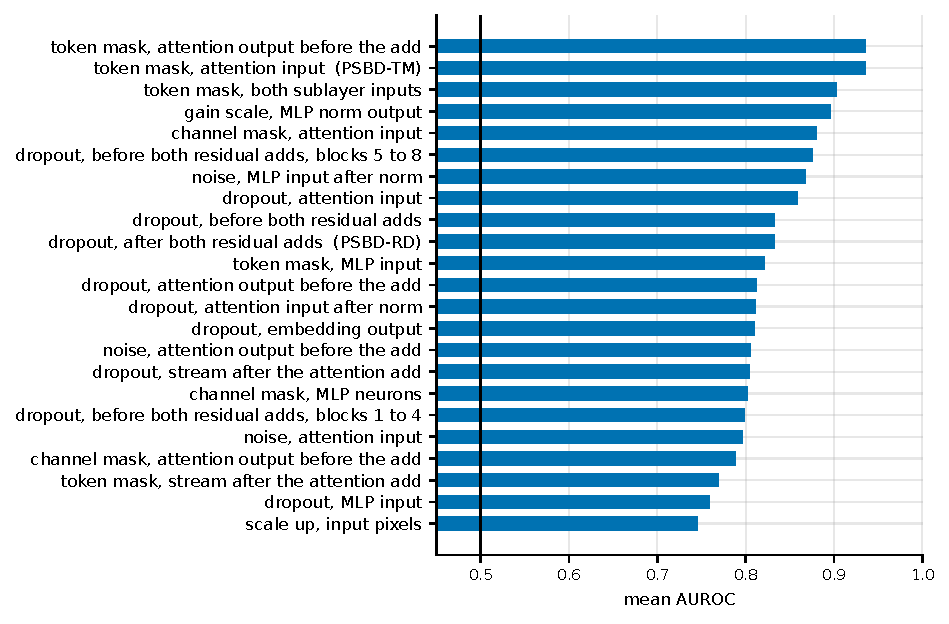
\includegraphics{basis_ranking.pdf}
\caption{Mean AUROC of every placement with a complete sweep, read at the rate the original rule assigns.}
\label{fig:basis}
\end{figure}
\FloatBarrier

\subsection{Depth bands at the adaptive rule}
\label{sec:results:depth}

PSBD-TM perturbs all \VitBlocks{} blocks. \Cref{tab:staircase-bands} restricts it to a third of the network at the adaptive rule. Restricting the mask to blocks 5 to 8 costs \StaircaseBandsBeforeAttentionNormBlocksFiveEightTokenMaskGain{} and to blocks 9 to 12 costs \StaircaseBandsBeforeAttentionNormBlocksNineOneTwoTokenMaskGain{}. Few models reach the shift target with the first third alone, so \cref{app:bands} compares the bands at matched disturbance, where the first third loses most.

% generated by scripts/paper/tab_staircase.py from results/coverage/coverage.json, results/<folder>/psbd_metrics.json (54 models) at 2026-09-29T18:12:06.471752+00:00, commit d73d3277d007fd75b3a4166a7911b1e07a2761b7-dirty. Do not edit by hand.
\begin{table*}[htbp]
\centering
\small
\caption{Token masking at the attention input of ViT-B/16, restricted to bands of blocks.}
\label{tab:staircase-bands}
\begin{tabular}{lrrrrl}
\toprule
 & & & \multicolumn{2}{c}{TPR@FPR} & \\
\cmidrule(lr){4-5}
Placement & n & AUROC & 10\% & 20\% & Gain [95\% CI] \\
\midrule
token mask, attention input, all 12 blocks & 54 & 0.963 & 0.887 & 0.916 & -- \\
token mask, attention input, blocks 1 to 4 & 11 & 0.949 & 0.867 & 0.949 & $-$0.031 [$-$0.044, $-$0.019] \\
token mask, attention input, blocks 5 to 8 & 35 & 0.891 & 0.788 & 0.864 & $-$0.087 [$-$0.143, $-$0.038] \\
token mask, attention input, blocks 9 to 12 & 25 & 0.955 & 0.891 & 0.936 & $-$0.023 [$-$0.045, $-$0.004] \\
\bottomrule
\end{tabular}
\end{table*}

\FloatBarrier

\subsection{Whether placements agree on which inputs are fragile}
\label{app:agreement}

If every placement read the same per-sample quantity, a union of placements could add nothing. \Cref{tab:mech-operator-agreement} gives the Spearman correlation between each placement's per-sample PSU and that of PSBD-TM, each read at its own matched rate. \Cref{tab:mech-operator-agreement-family} averages it within and across families of sites.

% generated by scripts/paper/mech_operator_agreement.py from results/<folder>/psbd/<placement>/rate_*_{clean,backdoor}.pt at 2026-09-30T13:04:41.000399+00:00, commit 257fa16f3d6cf6ee17ee984d58eef143db7ecc4c-dirty. Do not edit by hand.
\begin{table}[htbp]
\centering
\small
\caption{Whether placements agree on which inputs are fragile. Mean Spearman correlation, over the models whose attack succeeded, between each placement's per-sample fractional PSU and that of token masking at the attention input, each at its own matched 0.6 rate. n is the number of models carrying both placements at a usable rate.}
\label{tab:mech-operator-agreement}
\begin{adjustbox}{max width=\linewidth}
\begin{tabular}{lrrrrr}
\toprule
placement & family & rho, clean & n & rho, triggered & n \\
\midrule
channel mask, attention input & input side & 0.633 & 56 & 0.252 & 56 \\
noise, attention input & input side & 0.384 & 56 & 0.235 & 56 \\
token mask, MLP input & input side & 0.564 & 56 & 0.442 & 56 \\
token mask, both sublayer inputs & input side & 0.812 & 56 & 0.577 & 56 \\
scale up, input pixels & input side & 0.213 & 56 & 0.097 & 56 \\
noise, MLP input after norm & input side & 0.545 & 56 & 0.248 & 56 \\
token mask, attention output before the add & residual adjacent & 0.538 & 56 & 0.416 & 56 \\
token mask, stream after the attention add & residual adjacent & 0.577 & 56 & 0.443 & 56 \\
dropout, stream after the attention add & residual adjacent & 0.519 & 56 & 0.277 & 56 \\
dropout, before both residual adds & residual adjacent & 0.598 & 56 & 0.275 & 56 \\
dropout, after both residual adds & residual adjacent & 0.613 & 56 & 0.315 & 56 \\
channel mask, MLP neurons & structured & 0.504 & 56 & 0.173 & 56 \\
gain scale, MLP norm output & ported & 0.372 & 56 & 0.316 & 56 \\
token mask, attention input, blocks 5 to 8 & depth band & 0.570 & 56 & 0.434 & 56 \\
token mask, attention input, blocks 9 to 12 & depth band & 0.686 & 56 & 0.126 & 56 \\
dropout, before both residual adds, blocks 1 to 4 & depth band & 0.560 & 56 & 0.234 & 56 \\
dropout, before both residual adds, blocks 5 to 8 & depth band & 0.650 & 56 & 0.271 & 56 \\
dropout, before both residual adds, blocks 9 to 12 & depth band & 0.439 & 56 & 0.217 & 56 \\
dropout, attention input & input side & 0.660 & 56 & 0.272 & 56 \\
dropout, attention input after norm & input side & 0.407 & 56 & 0.180 & 56 \\
dropout, MLP input & input side & 0.479 & 56 & 0.186 & 56 \\
dropout, embedding output & input side & 0.391 & 56 & 0.190 & 56 \\
token mask, attention input, blocks 1 to 4 & depth band & 0.519 & 56 & 0.333 & 56 \\
dropout, attention output before the add & residual adjacent & 0.542 & 56 & 0.180 & 56 \\
channel mask, attention output before the add & residual adjacent & 0.514 & 56 & 0.185 & 56 \\
noise, attention output before the add & residual adjacent & 0.566 & 56 & 0.277 & 56 \\
\bottomrule
\end{tabular}
\end{adjustbox}
\end{table}

% generated by scripts/paper/mech_operator_agreement.py from results/<folder>/psbd/<placement>/rate_*_{clean,backdoor}.pt at 2026-09-24T04:33:16.351447+00:00, commit 52e4ba1a7ac941365bc37d68e1e902dad4fb4f74-dirty. Do not edit by hand.
\begin{table}[htbp]
\centering
\small
\caption{Mean per-sample PSU agreement, Spearman correlation averaged over placement pairs and over models, within and across the input-side and residual-adjacent families.}
\label{tab:mech-operator-agreement-family}
\begin{adjustbox}{max width=\linewidth}
\begin{tabular}{lrrrr}
\toprule
comparison & clean rho & n pairs & backdoor rho & n pairs \\
\midrule
within the input-side family & 0.469 & 55 & 0.256 & 55 \\
within the residual-adjacent family & 0.583 & 28 & 0.348 & 28 \\
across the 2 families & 0.512 & 88 & 0.298 & 88 \\
\bottomrule
\end{tabular}
\end{adjustbox}
\end{table}

\FloatBarrier

\subsection{PSU distributions}
\label{app:distributions}

\Cref{fig:psu} shows PSU on six models. In the top row, a BadNets, a BPP and a Blend model, the triggered inputs keep their prediction under the mask and pile up near 0, while the clean inputs lose theirs and pile up near 1. The threshold at the \HeadlineQuantilePercent{} percentile of the clean validation set sits between the two groups. The bottom row shows the three weakest readings. On WaNet and SIG on CIFAR-10 the triggered inputs move as much as the clean ones, so the histograms overlap. On TaCT on Tiny ImageNet both groups sit near 1 and only a thin tail of triggered inputs falls below the threshold.

\begin{figure}[htbp]
\centering
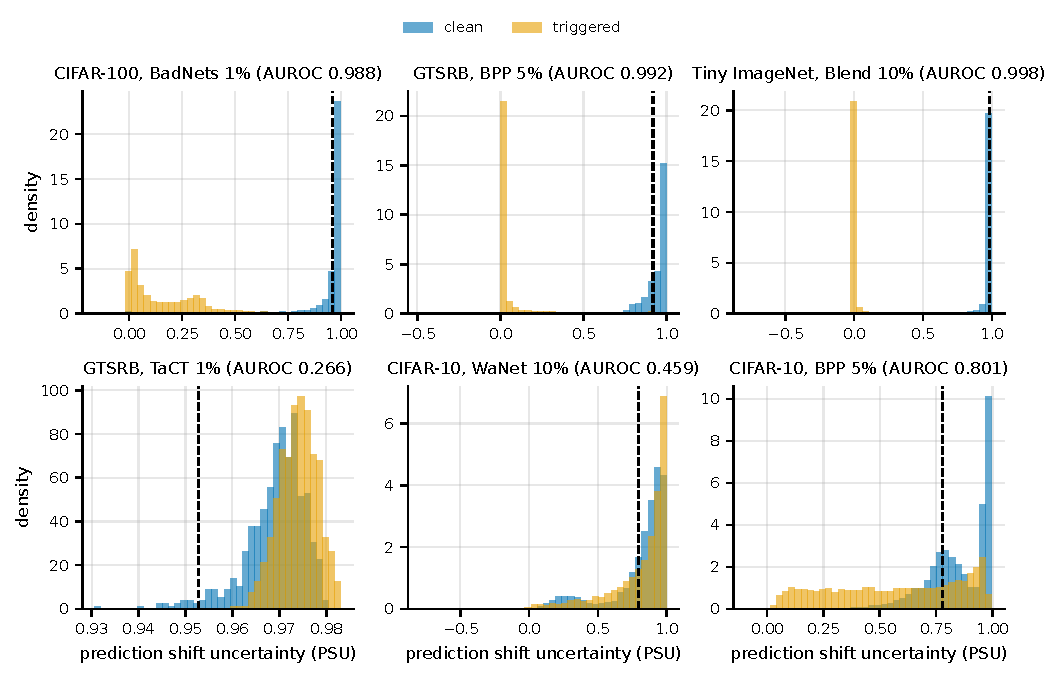
\includegraphics[width=\textwidth]{fig_psu_histograms.pdf}
\caption{PSU under PSBD-TM for clean and triggered inputs, with the threshold at the \HeadlineQuantilePercent{} percentile of the clean validation set (dashed). Top, three models where detection succeeds. Bottom, the three weakest readings.}
\label{fig:psu}
\end{figure}
\FloatBarrier
\clearpage


\section{Every detector per attack}
\label{supp:detectors}

\subsection{AUROC and true-positive rates}
\label{app:detectors}

\Cref{tab:detectors-auroc,tab:detectors-tpr10,tab:detectors-tpr20} and the tables that follow each of them give AUROC and the true-positive rate at 10\% and 20\% false-positive budgets for every defense on every model, one table per dataset. Every detector is read on the same models, splits and thresholds as PSBD. The threshold is set on the \HeldoutSize{} clean validation images so that the named share of them is flagged.

Two ports behave in ways specific to ViTs. SentiNet's Grad-CAM \cite{selvaraju2017gradcam} mask covers 0 to 2\% of the trigger at every block, so its transplant carries almost nothing of the trigger. That would explain a reading at chance, but its mean AUROC is \DetectorsAurocSentinet{}, below chance, so the port carries some signal with the wrong sign, which we report without an explanation. IBD-PSC at the paper's fixed amplification factor of \DetectorsIbdPscFactor{} saturates on a ViT because it keeps every prediction. It reads \DetectorsAurocIbdPsc{}, while the calibrated port that searches the factor per model reads \DetectorsAurocBestCompetitor{}. We therefore count only the calibrated port as the competitor.

% generated by scripts/paper/tab_detectors.py from results/coverage/coverage.json (57 of 59 clearing cells carry every defense), results/*/detectors/*_metrics.json, results/*/psbd_metrics.json at 2026-09-29T16:26:29.298213+00:00, commit 19488b81358b06040ba96f361d5061b2981f1f25-dirty. Do not edit by hand.
% generated by scripts/paper/tab_detectors.py from results/coverage/coverage.json (65 of 65 clearing cells carry every defense), results/*/detectors/*_metrics.json, results/*/psbd_metrics.json at 2026-09-24T04:50:59.131433+00:00, commit 9300709d1f6e7a0ba702f153d77765353ffa1368-dirty. Do not edit by hand.
\begin{table}[htbp]
\centering
\small
\caption{AUROC of every defense on CIFAR-10. Rows are attacks at their poison rate in percent and columns defenses, PSBD-TM first. Best in each row is bold and second best underlined, gray marks a reading below chance and shaded rows are means. PSBD-RD is our adaptation of the original PSBD site to a ViT block. Scale-Up$^\dagger$ is the data-limited variant and IBD-PSC$^\ast$ the calibrated one.}
\label{tab:detectors-auroc}
\begin{adjustbox}{max width=\linewidth}
\begin{tabular}{lrrrrrrrrrrrrr}
\toprule
attack, rate \% & \rotatebox{90}{PSBD-TM} & \rotatebox{90}{PSBD-RD} & \rotatebox{90}{Conf} & \rotatebox{90}{STRIP} & \rotatebox{90}{Scale-Up} & \rotatebox{90}{Scale-Up$^\dagger$} & \rotatebox{90}{IBD-PSC} & \rotatebox{90}{IBD-PSC$^\ast$} & \rotatebox{90}{TeCo} & \rotatebox{90}{CD-L} & \rotatebox{90}{Beatrix} & \rotatebox{90}{TED} & \rotatebox{90}{SentiNet} \\
\midrule
BadNets 1 & \textbf{0.982} & \textcolor{black!45}{0.309} & \textcolor{black!45}{0.479} & 0.906 & \underline{0.977} & 0.909 & 0.558 & 0.975 & 0.891 & 0.958 & 0.969 & 0.814 & 0.644 \\
BadNets 5 & \textbf{0.992} & 0.630 & 0.870 & 0.955 & 0.985 & 0.914 & 0.715 & 0.926 & 0.981 & \underline{0.991} & 0.986 & 0.813 & \textcolor{black!45}{0.433} \\
BadNets 10 & 0.991 & 0.720 & 0.878 & \underline{0.997} & 0.989 & 0.689 & 0.957 & 0.979 & 0.946 & \textbf{1.000} & 0.996 & 0.688 & 0.556 \\
Blend 1 & 0.922 & 0.990 & 0.706 & 0.984 & 0.931 & 0.668 & 0.864 & 0.989 & 0.908 & \underline{0.999} & \textbf{1.000} & 0.830 & \textcolor{black!45}{0.396} \\
Blend 5 & 0.971 & 0.984 & 0.890 & 0.955 & 0.930 & 0.617 & 0.885 & 0.990 & 0.895 & \underline{0.999} & \textbf{1.000} & 0.977 & 0.515 \\
Blend 10 & 0.906 & 0.991 & 0.701 & 0.960 & 0.846 & 0.587 & 0.808 & \underline{0.991} & 0.906 & 0.936 & \textbf{1.000} & 0.964 & \textcolor{black!45}{0.391} \\
BPP 1 & \underline{0.986} & 0.970 & \textcolor{black!45}{0.388} & 0.928 & \textcolor{black!45}{0.389} & \textcolor{black!45}{0.210} & \textcolor{black!45}{0.416} & 0.975 & \textcolor{black!45}{0.447} & 0.951 & \textbf{0.994} & 0.866 & \textcolor{black!45}{0.254} \\
BPP 5 & 0.801 & 0.880 & 0.523 & 0.907 & \textcolor{black!45}{0.413} & \textcolor{black!45}{0.158} & 0.541 & \underline{0.974} & \textcolor{black!45}{0.358} & 0.931 & \textbf{0.998} & 0.874 & \textcolor{black!45}{0.122} \\
BPP 10 & 0.871 & 0.875 & 0.738 & 0.950 & \textcolor{black!45}{0.455} & \textcolor{black!45}{0.221} & 0.841 & \underline{0.991} & \textcolor{black!45}{0.482} & 0.974 & \textbf{0.999} & 0.905 & \textcolor{black!45}{0.273} \\
LF 1 & \textbf{0.979} & \underline{0.941} & \textcolor{black!45}{0.268} & 0.729 & 0.787 & 0.646 & \textcolor{black!45}{0.371} & 0.877 & \textcolor{black!45}{0.467} & 0.806 & 0.940 & 0.808 & \textcolor{black!45}{0.268} \\
LF 5 & \textbf{0.991} & 0.959 & \textcolor{black!45}{0.392} & 0.952 & 0.949 & 0.696 & 0.501 & 0.955 & \textcolor{black!45}{0.285} & 0.923 & \underline{0.986} & 0.775 & \textcolor{black!45}{0.295} \\
LF 10 & \textbf{0.993} & \underline{0.977} & 0.780 & 0.914 & 0.909 & 0.685 & 0.613 & 0.883 & \textcolor{black!45}{0.377} & 0.907 & 0.961 & 0.860 & \textcolor{black!45}{0.284} \\
SIG 10 & \textcolor{black!45}{0.418} & 0.919 & 0.866 & 0.806 & 0.767 & 0.750 & 0.531 & 0.599 & 0.797 & 0.637 & \underline{0.992} & \textbf{0.997} & \textcolor{black!45}{0.005} \\
TaCT 1 & \underline{0.979} & \textcolor{black!45}{0.464} & \textcolor{black!45}{0.175} & 0.509 & 0.653 & \textcolor{black!45}{0.181} & \textcolor{black!45}{0.210} & 0.713 & 0.599 & \textcolor{black!45}{0.374} & \textbf{0.997} & 0.926 & \textcolor{black!45}{0.025} \\
TaCT 5 & 0.966 & 0.834 & 0.728 & 0.596 & \underline{0.981} & 0.876 & 0.850 & 0.855 & 0.881 & 0.710 & \textbf{0.998} & 0.970 & \textcolor{black!45}{0.076} \\
TaCT 10 & 0.963 & \textcolor{black!45}{0.261} & 0.975 & 0.797 & \underline{0.991} & 0.940 & 0.974 & 0.928 & 0.601 & 0.971 & \textbf{0.996} & 0.893 & \textcolor{black!45}{0.011} \\
WaNet 5 & 0.937 & \textbf{0.956} & \textcolor{black!45}{0.480} & 0.517 & 0.929 & \textcolor{black!45}{0.404} & 0.556 & 0.693 & \underline{0.946} & 0.729 & 0.714 & 0.810 & \textcolor{black!45}{0.461} \\
WaNet 10 & \textcolor{black!45}{0.459} & \textbf{0.947} & \textcolor{black!45}{0.376} & 0.504 & 0.567 & \textcolor{black!45}{0.380} & \textcolor{black!45}{0.448} & 0.687 & 0.732 & 0.579 & 0.827 & \underline{0.848} & \textcolor{black!45}{0.353} \\
\rowcolor{black!8}\emph{CIFAR-10 mean} & \underline{0.895} & 0.811 & 0.623 & 0.826 & 0.803 & 0.585 & 0.647 & 0.888 & 0.694 & 0.854 & \textbf{0.964} & 0.868 & \textcolor{black!45}{0.298} \\
\bottomrule
\end{tabular}
\end{adjustbox}
\end{table}

% generated by scripts/paper/tab_detectors.py from results/coverage/coverage.json (65 of 65 clearing cells carry every defense), results/*/detectors/*_metrics.json, results/*/psbd_metrics.json at 2026-09-24T04:51:05.458444+00:00, commit 9300709d1f6e7a0ba702f153d77765353ffa1368-dirty. Do not edit by hand.
\begin{table}[htbp]
\centering
\small
\caption{AUROC of every defense on CIFAR-100. Layout as in \cref{tab:detectors-auroc}.}
\label{tab:detectors-auroc-cifar-100}
\begin{adjustbox}{max width=\linewidth}
\begin{tabular}{lrrrrrrrrrrrrr}
\toprule
attack, rate \% & \rotatebox{90}{PSBD-TM} & \rotatebox{90}{PSBD-RD} & \rotatebox{90}{Conf} & \rotatebox{90}{STRIP} & \rotatebox{90}{Scale-Up} & \rotatebox{90}{Scale-Up$^\dagger$} & \rotatebox{90}{IBD-PSC} & \rotatebox{90}{IBD-PSC$^\ast$} & \rotatebox{90}{TeCo} & \rotatebox{90}{CD-L} & \rotatebox{90}{Beatrix} & \rotatebox{90}{TED} & \rotatebox{90}{SentiNet} \\
\midrule
BadNets 1 & 0.988 & 0.744 & 0.752 & 0.996 & 0.986 & 0.997 & 0.803 & 0.981 & 0.991 & \textbf{1.000} & \underline{0.997} & 0.990 & 0.978 \\
BadNets 5 & 0.994 & 0.826 & 0.980 & 0.993 & 0.989 & 0.992 & 0.959 & 0.972 & 0.994 & \textbf{1.000} & 0.878 & \underline{0.994} & 0.913 \\
BadNets 10 & \underline{0.998} & \textcolor{black!45}{0.497} & 0.965 & 0.995 & 0.992 & 0.998 & 0.982 & 0.990 & 0.993 & \textbf{0.999} & 0.998 & 0.979 & 0.967 \\
Blend 1 & 0.976 & 0.792 & 0.598 & 0.655 & 0.679 & 0.657 & 0.810 & 0.973 & \underline{0.987} & 0.860 & \textbf{0.990} & 0.983 & \textcolor{black!45}{0.317} \\
Blend 5 & 0.979 & \underline{0.999} & 0.958 & 0.897 & 0.782 & 0.730 & 0.931 & 0.987 & 0.976 & 0.953 & 0.984 & \textbf{1.000} & 0.899 \\
Blend 10 & \underline{0.998} & \textbf{1.000} & 0.966 & 0.995 & 0.916 & 0.778 & 0.992 & 0.997 & 0.872 & 0.938 & 0.972 & 0.951 & 0.764 \\
BPP 1 & 0.921 & \underline{0.950} & \textcolor{black!45}{0.375} & 0.819 & 0.530 & \textcolor{black!45}{0.258} & 0.622 & 0.875 & 0.561 & \textbf{0.967} & 0.902 & 0.940 & 0.855 \\
BPP 5 & 0.985 & \underline{0.988} & 0.910 & 0.952 & 0.675 & \textcolor{black!45}{0.244} & 0.870 & 0.937 & 0.917 & \textbf{0.993} & 0.983 & 0.982 & 0.805 \\
BPP 10 & 0.985 & \underline{0.985} & 0.853 & 0.942 & 0.646 & \textcolor{black!45}{0.328} & 0.848 & 0.967 & 0.724 & 0.984 & \textbf{0.986} & 0.981 & 0.602 \\
LF 1 & 0.956 & 0.956 & 0.657 & 0.753 & 0.701 & 0.595 & 0.815 & 0.920 & 0.674 & \textcolor{black!45}{0.383} & \textbf{0.958} & \underline{0.956} & \textcolor{black!45}{0.499} \\
LF 5 & \underline{0.967} & 0.966 & 0.807 & 0.632 & 0.608 & 0.562 & \textcolor{black!45}{0.463} & 0.760 & 0.597 & \textcolor{black!45}{0.261} & 0.957 & \textbf{0.975} & 0.815 \\
LF 10 & \textbf{0.995} & 0.982 & 0.932 & 0.882 & 0.599 & 0.549 & 0.907 & 0.952 & \textcolor{black!45}{0.408} & \textcolor{black!45}{0.377} & 0.972 & \underline{0.983} & 0.730 \\
TaCT 1 & 0.909 & \textcolor{black!45}{0.493} & 0.919 & 0.673 & 0.668 & 0.622 & \textbf{0.935} & \underline{0.931} & 0.908 & 0.772 & 0.604 & 0.650 & \textcolor{black!45}{0.338} \\
TaCT 5 & 0.933 & 0.554 & \textbf{0.998} & 0.975 & \underline{0.997} & 0.995 & 0.983 & 0.980 & 0.921 & 0.956 & 0.658 & 0.636 & \textcolor{black!45}{0.307} \\
TaCT 10 & 0.891 & \textcolor{black!45}{0.488} & \textbf{0.982} & 0.738 & 0.977 & \underline{0.982} & 0.971 & 0.966 & 0.918 & 0.961 & 0.629 & 0.664 & \textcolor{black!45}{0.308} \\
\rowcolor{black!8}\emph{CIFAR-100 mean} & \textbf{0.965} & 0.815 & 0.844 & 0.860 & 0.783 & 0.686 & 0.859 & \underline{0.946} & 0.829 & 0.827 & 0.898 & 0.911 & 0.673 \\
\bottomrule
\end{tabular}
\end{adjustbox}
\end{table}

% generated by scripts/paper/tab_detectors.py from results/coverage/coverage.json (65 of 65 clearing cells carry every defense), results/*/detectors/*_metrics.json, results/*/psbd_metrics.json at 2026-09-24T04:51:11.873676+00:00, commit 9300709d1f6e7a0ba702f153d77765353ffa1368-dirty. Do not edit by hand.
\begin{table}[htbp]
\centering
\small
\caption{AUROC of every defense on GTSRB. Layout as in \cref{tab:detectors-auroc}.}
\label{tab:detectors-auroc-gtsrb}
\begin{adjustbox}{max width=\linewidth}
\begin{tabular}{lrrrrrrrrrrrrr}
\toprule
attack, rate \% & \rotatebox{90}{PSBD-TM} & \rotatebox{90}{PSBD-RD} & \rotatebox{90}{Conf} & \rotatebox{90}{STRIP} & \rotatebox{90}{Scale-Up} & \rotatebox{90}{Scale-Up$^\dagger$} & \rotatebox{90}{IBD-PSC} & \rotatebox{90}{IBD-PSC$^\ast$} & \rotatebox{90}{TeCo} & \rotatebox{90}{CD-L} & \rotatebox{90}{Beatrix} & \rotatebox{90}{TED} & \rotatebox{90}{SentiNet} \\
\midrule
BadNets 1 & 0.999 & \textcolor{black!45}{0.222} & \textcolor{black!45}{0.292} & 0.995 & 0.908 & \textbf{1.000} & 0.630 & 0.929 & 0.982 & 0.980 & \underline{1.000} & 0.999 & \textcolor{black!45}{0.122} \\
BadNets 5 & 1.000 & 0.889 & 0.726 & \textbf{1.000} & 0.914 & \textbf{1.000} & 0.506 & 0.999 & 0.996 & \underline{1.000} & 1.000 & 0.998 & \textcolor{black!45}{0.090} \\
BadNets 10 & \underline{1.000} & 0.999 & \textcolor{black!45}{0.299} & 0.979 & 0.901 & \textbf{1.000} & \textcolor{black!45}{0.328} & 0.993 & 0.954 & 1.000 & 1.000 & 0.999 & \textcolor{black!45}{0.137} \\
Blend 1 & \underline{1.000} & 0.999 & \textcolor{black!45}{0.165} & 0.963 & 0.679 & 0.873 & \textcolor{black!45}{0.410} & 1.000 & 0.771 & 0.936 & \textbf{1.000} & 1.000 & \textcolor{black!45}{0.220} \\
Blend 5 & \underline{0.999} & 0.899 & 0.876 & 0.977 & 0.686 & 0.941 & 0.970 & 0.993 & 0.918 & 0.982 & \textbf{1.000} & 0.996 & \textcolor{black!45}{0.323} \\
Blend 10 & \textbf{1.000} & 0.998 & \textcolor{black!45}{0.413} & 0.966 & 0.692 & 0.944 & 0.993 & \underline{1.000} & 0.831 & 0.998 & 1.000 & 0.999 & \textcolor{black!45}{0.302} \\
BPP 1 & 0.898 & 0.755 & \textcolor{black!45}{0.035} & \textcolor{black!45}{0.148} & \textcolor{black!45}{0.245} & \textcolor{black!45}{0.428} & \textcolor{black!45}{0.071} & 0.921 & \textcolor{black!45}{0.498} & 0.935 & \textbf{0.989} & \underline{0.940} & 0.699 \\
BPP 5 & 0.992 & 0.994 & 0.637 & 0.914 & \textcolor{black!45}{0.144} & \textcolor{black!45}{0.359} & \textcolor{black!45}{0.352} & 0.821 & \textcolor{black!45}{0.284} & 0.985 & \textbf{0.999} & \underline{0.995} & \textcolor{black!45}{0.197} \\
BPP 10 & 0.989 & 0.977 & 0.579 & 0.892 & \textcolor{black!45}{0.148} & \textcolor{black!45}{0.393} & \textcolor{black!45}{0.330} & 0.738 & \textcolor{black!45}{0.350} & 0.967 & \textbf{0.999} & \underline{0.997} & \textcolor{black!45}{0.121} \\
LF 1 & 0.976 & 0.987 & \textcolor{black!45}{0.133} & 0.813 & 0.606 & 0.894 & \textcolor{black!45}{0.226} & 0.954 & 0.661 & \textcolor{black!45}{0.295} & \textbf{0.995} & \underline{0.988} & \textcolor{black!45}{0.126} \\
LF 5 & \underline{0.998} & 0.997 & \textcolor{black!45}{0.491} & 0.942 & 0.742 & 0.917 & \textcolor{black!45}{0.384} & 0.969 & \textcolor{black!45}{0.122} & 0.688 & \textbf{0.999} & 0.993 & \textcolor{black!45}{0.007} \\
LF 10 & 0.998 & 0.999 & 0.598 & 0.960 & 0.656 & 0.870 & 0.705 & 0.951 & \textcolor{black!45}{0.146} & 0.625 & \underline{0.999} & \textbf{1.000} & \textcolor{black!45}{0.473} \\
TaCT 5 & 0.942 & \textcolor{black!45}{0.392} & 0.999 & 0.862 & 0.992 & \underline{1.000} & 0.991 & 0.981 & 0.995 & 0.521 & \textbf{1.000} & 0.999 & \textcolor{black!45}{0.001} \\
TaCT 10 & 0.748 & \textcolor{black!45}{0.295} & 0.999 & 0.979 & 0.994 & \textbf{1.000} & \underline{0.999} & 0.991 & 0.969 & 0.940 & 0.734 & \textcolor{black!45}{0.370} & 0.711 \\
WaNet 10 & 0.948 & \underline{0.960} & \textcolor{black!45}{0.482} & 0.504 & 0.529 & \textcolor{black!45}{0.427} & \textcolor{black!45}{0.475} & 0.643 & 0.948 & 0.549 & 0.667 & \textbf{0.964} & \textcolor{black!45}{0.239} \\
\rowcolor{black!8}\emph{GTSRB mean} & \textbf{0.966} & 0.824 & 0.515 & 0.860 & 0.656 & 0.803 & 0.558 & 0.925 & 0.695 & 0.827 & \underline{0.959} & 0.949 & \textcolor{black!45}{0.251} \\
\bottomrule
\end{tabular}
\end{adjustbox}
\end{table}

% generated by scripts/paper/tab_detectors.py from results/coverage/coverage.json (65 of 65 clearing cells carry every defense), results/*/detectors/*_metrics.json, results/*/psbd_metrics.json at 2026-09-24T04:51:18.433986+00:00, commit 9300709d1f6e7a0ba702f153d77765353ffa1368-dirty. Do not edit by hand.
\begin{table}[htbp]
\centering
\small
\caption{AUROC of every defense on Tiny ImageNet. Layout as in \cref{tab:detectors-auroc}.}
\label{tab:detectors-auroc-tiny-imagenet}
\begin{adjustbox}{max width=\linewidth}
\begin{tabular}{lrrrrrrrrrrrrr}
\toprule
attack, rate \% & \rotatebox{90}{PSBD-TM} & \rotatebox{90}{PSBD-RD} & \rotatebox{90}{Conf} & \rotatebox{90}{STRIP} & \rotatebox{90}{Scale-Up} & \rotatebox{90}{Scale-Up$^\dagger$} & \rotatebox{90}{IBD-PSC} & \rotatebox{90}{IBD-PSC$^\ast$} & \rotatebox{90}{TeCo} & \rotatebox{90}{CD-L} & \rotatebox{90}{Beatrix} & \rotatebox{90}{TED} & \rotatebox{90}{SentiNet} \\
\midrule
BadNets 1 & 0.980 & 0.892 & 0.741 & 0.922 & \underline{0.991} & 0.989 & 0.901 & 0.961 & \textbf{0.993} & 0.708 & 0.851 & 0.930 & \textcolor{black!45}{0.438} \\
BadNets 5 & 0.984 & 0.837 & 0.939 & 0.949 & \underline{0.993} & 0.958 & 0.932 & 0.942 & \textbf{0.995} & 0.839 & 0.763 & 0.863 & \textcolor{black!45}{0.394} \\
BadNets 10 & \underline{0.993} & 0.973 & 0.978 & 0.931 & \textbf{0.995} & 0.940 & 0.949 & 0.957 & 0.991 & 0.846 & 0.557 & 0.840 & \textcolor{black!45}{0.312} \\
Blend 1 & 0.992 & \underline{0.996} & 0.886 & 0.832 & 0.851 & 0.686 & 0.942 & \textbf{0.998} & 0.928 & 0.577 & 0.888 & 0.691 & \textcolor{black!45}{0.370} \\
Blend 5 & 0.997 & \textbf{0.999} & 0.943 & 0.910 & 0.892 & 0.687 & 0.972 & \underline{0.999} & 0.931 & 0.619 & 0.624 & 0.684 & \textcolor{black!45}{0.175} \\
Blend 10 & 0.998 & \textbf{0.999} & 0.995 & 0.975 & 0.950 & 0.724 & 0.993 & \underline{0.999} & 0.955 & \textcolor{black!45}{0.408} & 0.579 & 0.677 & \textcolor{black!45}{0.497} \\
BPP 1 & \underline{0.980} & \textbf{0.981} & 0.833 & 0.953 & \textcolor{black!45}{0.459} & \textcolor{black!45}{0.184} & 0.959 & 0.977 & 0.755 & 0.722 & 0.727 & 0.709 & 0.653 \\
BPP 5 & \underline{0.987} & \textbf{0.987} & 0.909 & 0.940 & \textcolor{black!45}{0.337} & \textcolor{black!45}{0.077} & 0.970 & 0.977 & 0.634 & 0.817 & 0.736 & 0.852 & 0.626 \\
BPP 10 & \underline{0.984} & \textbf{0.997} & 0.858 & 0.964 & \textcolor{black!45}{0.346} & \textcolor{black!45}{0.058} & 0.886 & 0.886 & 0.732 & 0.827 & 0.804 & 0.647 & \textcolor{black!45}{0.417} \\
LF 1 & \underline{0.941} & \textbf{0.952} & 0.767 & 0.608 & 0.710 & 0.628 & 0.876 & 0.876 & 0.692 & 0.783 & 0.632 & 0.710 & \textcolor{black!45}{0.298} \\
LF 5 & \underline{0.987} & \textbf{0.991} & 0.951 & 0.845 & 0.813 & \textcolor{black!45}{0.455} & 0.972 & 0.972 & 0.542 & \textcolor{black!45}{0.483} & 0.507 & 0.557 & \textcolor{black!45}{0.380} \\
LF 10 & \underline{0.973} & \textbf{0.982} & 0.926 & 0.733 & 0.734 & 0.630 & 0.954 & 0.954 & 0.748 & 0.660 & 0.856 & 0.686 & \textcolor{black!45}{0.466} \\
TaCT 1 & 0.575 & \textcolor{black!45}{0.487} & \textbf{0.827} & 0.545 & 0.536 & \textcolor{black!45}{0.429} & 0.773 & \underline{0.776} & 0.618 & \textcolor{black!45}{0.329} & \textcolor{black!45}{0.449} & 0.532 & \textcolor{black!45}{0.411} \\
TaCT 5 & 0.663 & \textcolor{black!45}{0.488} & \underline{0.845} & 0.561 & 0.518 & \textcolor{black!45}{0.496} & \textbf{0.850} & \textbf{0.850} & 0.673 & \textcolor{black!45}{0.252} & 0.645 & \textcolor{black!45}{0.481} & 0.554 \\
TaCT 10 & \underline{0.810} & \textcolor{black!45}{0.417} & \textbf{0.840} & 0.501 & 0.549 & \textcolor{black!45}{0.477} & 0.668 & 0.668 & 0.595 & \textcolor{black!45}{0.364} & \textcolor{black!45}{0.461} & 0.541 & \textcolor{black!45}{0.488} \\
WaNet 5 & \underline{0.930} & \textbf{0.953} & 0.721 & 0.538 & 0.500 & \textcolor{black!45}{0.312} & 0.859 & 0.859 & 0.927 & 0.755 & \textcolor{black!45}{0.228} & 0.638 & \textcolor{black!45}{0.325} \\
WaNet 10 & 0.950 & \textbf{0.966} & 0.836 & 0.532 & 0.549 & \textcolor{black!45}{0.290} & 0.864 & 0.864 & \underline{0.955} & 0.906 & \textcolor{black!45}{0.414} & 0.772 & \textcolor{black!45}{0.364} \\
\rowcolor{black!8}\emph{Tiny ImageNet mean} & \textbf{0.925} & 0.876 & 0.870 & 0.779 & 0.690 & 0.531 & 0.901 & \underline{0.913} & 0.804 & 0.641 & 0.631 & 0.695 & \textcolor{black!45}{0.422} \\
\rowcolor{black!8}\emph{all models} & \textbf{0.935} & 0.832 & 0.714 & 0.829 & 0.735 & 0.644 & 0.742 & \underline{0.916} & 0.754 & 0.786 & 0.860 & 0.851 & \textcolor{black!45}{0.406} \\
\bottomrule
\end{tabular}
\end{adjustbox}
\end{table}


\FloatBarrier
% generated by scripts/paper/tab_detectors.py from results/coverage/coverage.json (56 of 62 successful cells carry every defense), results/*/detectors/*_metrics.json, results/*/psbd_metrics.json at 2026-09-30T13:11:35.728949+00:00, commit 257fa16f3d6cf6ee17ee984d58eef143db7ecc4c-dirty. Do not edit by hand.
% generated by scripts/paper/tab_detectors.py from results/coverage/coverage.json (57 of 59 clearing cells carry every defense), results/*/detectors/*_metrics.json, results/*/psbd_metrics.json at 2026-09-24T06:01:30.811386+00:00, commit 872fbbbd1f025c8c9924211876e2cda72fc45aab-dirty. Do not edit by hand.
\begin{table}[htbp]
\centering
\small
\caption{TPR at a 10\% false-positive budget of every defense on CIFAR-10. Rows are attacks at their poison rate in percent and columns defenses, PSBD-TM first. Best in each row is bold and second best underlined, gray marks a reading below chance and shaded rows are means. PSBD-RD is our adaptation of the original PSBD site to a ViT block. Scale-Up$^\dagger$ is the data-limited variant and IBD-PSC$^\ast$ the calibrated one.}
\label{tab:detectors-tpr10}
\begin{adjustbox}{max width=\linewidth}
\begin{tabular}{lrrrrrrrrrrrrr}
\toprule
attack, rate \% & \rotatebox{90}{PSBD-TM} & \rotatebox{90}{PSBD-RD} & \rotatebox{90}{Conf} & \rotatebox{90}{STRIP} & \rotatebox{90}{Scale-Up} & \rotatebox{90}{Scale-Up$^\dagger$} & \rotatebox{90}{IBD-PSC} & \rotatebox{90}{IBD-PSC$^\ast$} & \rotatebox{90}{TeCo} & \rotatebox{90}{CD-L} & \rotatebox{90}{Beatrix} & \rotatebox{90}{TED} & \rotatebox{90}{SentiNet} \\
\midrule
BadNets 1 & 0.959 & \textcolor{black!45}{0.015} & \textcolor{black!45}{0.000} & 0.652 & \textbf{0.997} & \textcolor{black!45}{0.000} & \textcolor{black!45}{0.000} & 0.967 & 0.685 & 0.891 & \underline{0.981} & 0.569 & \textcolor{black!45}{0.201} \\
BadNets 5 & 0.965 & \textcolor{black!45}{0.031} & 0.641 & 0.875 & \textbf{1.000} & \textcolor{black!45}{0.000} & \textcolor{black!45}{0.018} & 0.819 & 0.966 & 0.972 & \underline{0.998} & 0.517 & \textcolor{black!45}{0.119} \\
BadNets 10 & 0.935 & \textcolor{black!45}{0.113} & \textcolor{black!45}{0.486} & \textbf{1.000} & \textcolor{black!45}{0.000} & \textcolor{black!45}{0.000} & 0.947 & \underline{0.992} & 0.882 & \textbf{1.000} & \textbf{1.000} & \textcolor{black!45}{0.291} & \textcolor{black!45}{0.222} \\
Blend 1 & 0.773 & 0.983 & \textcolor{black!45}{0.002} & 0.951 & 0.637 & \textcolor{black!45}{0.000} & \textcolor{black!45}{0.140} & \underline{0.998} & 0.764 & 0.996 & \textbf{1.000} & 0.556 & \textcolor{black!45}{0.000} \\
Blend 5 & 0.908 & 0.973 & 0.633 & 0.885 & 0.553 & \textcolor{black!45}{0.000} & 0.670 & 0.997 & 0.689 & \underline{0.998} & \textbf{1.000} & 0.947 & \textcolor{black!45}{0.000} \\
Blend 10 & 0.754 & \underline{0.980} & \textcolor{black!45}{0.004} & 0.853 & \textcolor{black!45}{0.375} & \textcolor{black!45}{0.000} & \textcolor{black!45}{0.000} & \textbf{1.000} & 0.759 & 0.646 & \textbf{1.000} & 0.917 & \textcolor{black!45}{0.008} \\
BPP 1 & 0.956 & 0.897 & \textcolor{black!45}{0.000} & 0.810 & \textcolor{black!45}{0.010} & \textcolor{black!45}{0.010} & \textcolor{black!45}{0.000} & \underline{0.977} & \textcolor{black!45}{0.011} & 0.877 & \textbf{0.985} & 0.642 & \textcolor{black!45}{0.001} \\
BPP 5 & 0.587 & 0.673 & \textcolor{black!45}{0.000} & 0.760 & \textcolor{black!45}{0.010} & \textcolor{black!45}{0.008} & \textcolor{black!45}{0.000} & \underline{0.955} & \textcolor{black!45}{0.014} & 0.856 & \textbf{0.996} & 0.615 & \textcolor{black!45}{0.000} \\
BPP 10 & 0.736 & 0.720 & \textcolor{black!45}{0.013} & 0.881 & \textcolor{black!45}{0.001} & \textcolor{black!45}{0.001} & \textcolor{black!45}{0.041} & \underline{0.990} & \textcolor{black!45}{0.003} & 0.944 & \textbf{0.999} & 0.761 & \textcolor{black!45}{0.001} \\
LF 1 & \textbf{0.954} & 0.753 & \textcolor{black!45}{0.000} & \textcolor{black!45}{0.368} & \textcolor{black!45}{0.379} & \textcolor{black!45}{0.379} & \textcolor{black!45}{0.000} & 0.673 & \textcolor{black!45}{0.133} & \textcolor{black!45}{0.457} & \underline{0.851} & 0.550 & \textcolor{black!45}{0.000} \\
LF 5 & \textbf{0.983} & 0.837 & \textcolor{black!45}{0.000} & 0.867 & 0.762 & \textcolor{black!45}{0.000} & \textcolor{black!45}{0.000} & 0.875 & \textcolor{black!45}{0.033} & 0.722 & \underline{0.970} & 0.502 & \textcolor{black!45}{0.000} \\
LF 10 & \textbf{0.995} & 0.908 & \textcolor{black!45}{0.125} & 0.762 & 0.642 & \textcolor{black!45}{0.000} & \textcolor{black!45}{0.003} & 0.572 & \textcolor{black!45}{0.086} & 0.596 & \underline{0.941} & 0.643 & \textcolor{black!45}{0.001} \\
SIG 10 & \textcolor{black!45}{0.071} & 0.810 & 0.753 & 0.562 & \textcolor{black!45}{0.437} & \textcolor{black!45}{0.437} & \textcolor{black!45}{0.295} & \textcolor{black!45}{0.138} & \textcolor{black!45}{0.296} & \textcolor{black!45}{0.038} & \underline{0.985} & \textbf{0.995} & \textcolor{black!45}{0.002} \\
TaCT 1 & \textcolor{black!45}{0.005} & \textcolor{black!45}{0.013} & \textcolor{black!45}{0.000} & \textcolor{black!45}{0.089} & \textcolor{black!45}{0.131} & \textcolor{black!45}{0.004} & \textcolor{black!45}{0.000} & \textcolor{black!45}{0.134} & \textcolor{black!45}{0.098} & \textcolor{black!45}{0.005} & \textbf{0.994} & \underline{0.853} & \textcolor{black!45}{0.006} \\
TaCT 5 & \textcolor{black!45}{0.000} & \textcolor{black!45}{0.006} & \textcolor{black!45}{0.098} & \textcolor{black!45}{0.141} & 0.823 & 0.691 & \textcolor{black!45}{0.005} & \textcolor{black!45}{0.270} & \textcolor{black!45}{0.310} & \textcolor{black!45}{0.057} & \textbf{0.987} & \underline{0.950} & \textcolor{black!45}{0.000} \\
WaNet 5 & 0.838 & \textbf{0.908} & \textcolor{black!45}{0.000} & \textcolor{black!45}{0.089} & \textcolor{black!45}{0.000} & \textcolor{black!45}{0.005} & \textcolor{black!45}{0.000} & \textcolor{black!45}{0.174} & \underline{0.907} & \textcolor{black!45}{0.378} & \textcolor{black!45}{0.334} & 0.559 & \textcolor{black!45}{0.064} \\
WaNet 10 & \textcolor{black!45}{0.087} & \textbf{0.846} & \textcolor{black!45}{0.000} & \textcolor{black!45}{0.115} & \textcolor{black!45}{0.164} & \textcolor{black!45}{0.060} & \textcolor{black!45}{0.001} & \textcolor{black!45}{0.199} & \textcolor{black!45}{0.361} & \textcolor{black!45}{0.304} & 0.533 & \underline{0.656} & \textcolor{black!45}{0.014} \\
\rowcolor{black!8}\emph{CIFAR-10 mean} & 0.677 & 0.616 & \textcolor{black!45}{0.162} & 0.627 & \textcolor{black!45}{0.407} & \textcolor{black!45}{0.094} & \textcolor{black!45}{0.125} & \underline{0.690} & \textcolor{black!45}{0.412} & 0.631 & \textbf{0.915} & 0.678 & \textcolor{black!45}{0.038} \\
\bottomrule
\end{tabular}
\end{adjustbox}
\end{table}

% generated by scripts/paper/tab_detectors.py from results/coverage/coverage.json (65 of 65 clearing cells carry every defense), results/*/detectors/*_metrics.json, results/*/psbd_metrics.json at 2026-09-24T04:51:48.787049+00:00, commit 9300709d1f6e7a0ba702f153d77765353ffa1368-dirty. Do not edit by hand.
\begin{table}[htbp]
\centering
\small
\caption{TPR at a 10\% false-positive budget of every defense on CIFAR-100. Layout as in \cref{tab:detectors-tpr10}.}
\label{tab:detectors-tpr10-cifar-100}
\begin{adjustbox}{max width=\linewidth}
\begin{tabular}{lrrrrrrrrrrrrr}
\toprule
attack, rate \% & \rotatebox{90}{PSBD-TM} & \rotatebox{90}{PSBD-RD} & \rotatebox{90}{Conf} & \rotatebox{90}{STRIP} & \rotatebox{90}{Scale-Up} & \rotatebox{90}{Scale-Up$^\dagger$} & \rotatebox{90}{IBD-PSC} & \rotatebox{90}{IBD-PSC$^\ast$} & \rotatebox{90}{TeCo} & \rotatebox{90}{CD-L} & \rotatebox{90}{Beatrix} & \rotatebox{90}{TED} & \rotatebox{90}{SentiNet} \\
\midrule
BadNets 1 & 0.999 & \textcolor{black!45}{0.244} & \textcolor{black!45}{0.017} & \textbf{1.000} & 1.000 & \underline{1.000} & \textcolor{black!45}{0.000} & 0.973 & 0.998 & \textbf{1.000} & \textbf{1.000} & 0.975 & 0.932 \\
BadNets 5 & \underline{0.999} & \textcolor{black!45}{0.335} & 0.958 & \textbf{1.000} & \textbf{1.000} & \textbf{1.000} & 0.841 & 0.984 & 0.998 & \textbf{1.000} & \textcolor{black!45}{0.004} & 0.989 & 0.730 \\
BadNets 10 & \textbf{1.000} & \textcolor{black!45}{0.114} & 0.924 & \underline{0.999} & \textbf{1.000} & \textbf{1.000} & 0.994 & 0.987 & 0.999 & \textbf{1.000} & \textbf{1.000} & 0.941 & 0.895 \\
Blend 1 & 0.959 & \textcolor{black!45}{0.347} & \textcolor{black!45}{0.000} & \textcolor{black!45}{0.274} & \textcolor{black!45}{0.335} & \textcolor{black!45}{0.334} & \textcolor{black!45}{0.126} & 0.979 & \underline{0.986} & \textcolor{black!45}{0.423} & \textbf{0.989} & 0.973 & \textcolor{black!45}{0.003} \\
Blend 5 & 0.941 & 0.999 & 0.960 & 0.736 & \textcolor{black!45}{0.266} & \textcolor{black!45}{0.266} & 0.810 & \underline{1.000} & 0.919 & 0.887 & 0.996 & \textbf{1.000} & \textcolor{black!45}{0.459} \\
Blend 10 & \textbf{1.000} & \underline{1.000} & 0.928 & 0.989 & 0.602 & \textcolor{black!45}{0.348} & 0.999 & \textbf{1.000} & \textcolor{black!45}{0.291} & 0.911 & 0.854 & 0.910 & \textcolor{black!45}{0.008} \\
BPP 1 & 0.849 & \textbf{0.914} & \textcolor{black!45}{0.001} & 0.545 & \textcolor{black!45}{0.264} & \textcolor{black!45}{0.008} & \textcolor{black!45}{0.001} & 0.607 & \textcolor{black!45}{0.076} & \underline{0.901} & \textcolor{black!45}{0.038} & 0.898 & \textcolor{black!45}{0.242} \\
BPP 5 & 0.961 & \underline{0.973} & 0.811 & 0.893 & \textcolor{black!45}{0.002} & \textcolor{black!45}{0.001} & 0.523 & 0.824 & 0.752 & \textbf{0.983} & 0.884 & 0.963 & \textcolor{black!45}{0.029} \\
BPP 10 & \underline{0.963} & 0.960 & \textcolor{black!45}{0.486} & 0.860 & \textcolor{black!45}{0.001} & \textcolor{black!45}{0.001} & \textcolor{black!45}{0.260} & 0.948 & \textcolor{black!45}{0.266} & \textbf{0.977} & 0.923 & 0.960 & \textcolor{black!45}{0.022} \\
LF 1 & \textbf{0.942} & 0.903 & \textcolor{black!45}{0.029} & \textcolor{black!45}{0.477} & \textcolor{black!45}{0.233} & \textcolor{black!45}{0.230} & 0.539 & 0.815 & \textcolor{black!45}{0.247} & \textcolor{black!45}{0.049} & 0.887 & \underline{0.917} & \textcolor{black!45}{0.033} \\
LF 5 & \textbf{0.954} & 0.934 & 0.590 & \textcolor{black!45}{0.299} & \textcolor{black!45}{0.117} & \textcolor{black!45}{0.219} & \textcolor{black!45}{0.031} & \textcolor{black!45}{0.243} & \textcolor{black!45}{0.083} & \textcolor{black!45}{0.030} & \textcolor{black!45}{0.366} & \underline{0.949} & \textcolor{black!45}{0.203} \\
LF 10 & \textbf{0.995} & \underline{0.959} & 0.858 & 0.706 & \textcolor{black!45}{0.163} & \textcolor{black!45}{0.162} & 0.765 & 0.920 & \textcolor{black!45}{0.014} & \textcolor{black!45}{0.010} & 0.688 & 0.950 & \textcolor{black!45}{0.001} \\
TaCT 1 & 0.506 & \textcolor{black!45}{0.023} & \underline{0.632} & \textcolor{black!45}{0.184} & \textcolor{black!45}{0.069} & \textcolor{black!45}{0.184} & 0.575 & \textcolor{black!45}{0.218} & \textcolor{black!45}{0.138} & \textcolor{black!45}{0.000} & \textcolor{black!45}{0.000} & \textbf{0.966} & \textcolor{black!45}{0.046} \\
TaCT 5 & 0.540 & \textcolor{black!45}{0.218} & 0.690 & 0.920 & \textbf{0.977} & \textbf{0.977} & 0.586 & 0.736 & 0.552 & \textcolor{black!45}{0.241} & \textcolor{black!45}{0.000} & \underline{0.943} & \textcolor{black!45}{0.080} \\
TaCT 10 & \textcolor{black!45}{0.161} & \textcolor{black!45}{0.000} & 0.724 & \textcolor{black!45}{0.195} & \underline{0.931} & \underline{0.931} & \textcolor{black!45}{0.345} & 0.690 & \textcolor{black!45}{0.379} & \textcolor{black!45}{0.115} & \textcolor{black!45}{0.000} & \textbf{0.943} & \textcolor{black!45}{0.057} \\
\rowcolor{black!8}\emph{CIFAR-100 mean} & \underline{0.851} & 0.595 & 0.574 & 0.672 & \textcolor{black!45}{0.464} & \textcolor{black!45}{0.444} & \textcolor{black!45}{0.493} & 0.795 & 0.513 & 0.569 & 0.575 & \textbf{0.952} & \textcolor{black!45}{0.249} \\
\bottomrule
\end{tabular}
\end{adjustbox}
\end{table}

% generated by scripts/paper/tab_detectors.py from results/coverage/coverage.json (57 of 59 clearing cells carry every defense), results/*/detectors/*_metrics.json, results/*/psbd_metrics.json at 2026-09-24T06:01:44.703285+00:00, commit 872fbbbd1f025c8c9924211876e2cda72fc45aab-dirty. Do not edit by hand.
\begin{table}[htbp]
\centering
\small
\caption{TPR at a 10\% false-positive budget of every defense on GTSRB. Layout as in \cref{tab:detectors-tpr10}.}
\label{tab:detectors-tpr10-gtsrb}
\begin{adjustbox}{max width=\linewidth}
\begin{tabular}{lrrrrrrrrrrrrr}
\toprule
attack, rate \% & \rotatebox{90}{PSBD-TM} & \rotatebox{90}{PSBD-RD} & \rotatebox{90}{Conf} & \rotatebox{90}{STRIP} & \rotatebox{90}{Scale-Up} & \rotatebox{90}{Scale-Up$^\dagger$} & \rotatebox{90}{IBD-PSC} & \rotatebox{90}{IBD-PSC$^\ast$} & \rotatebox{90}{TeCo} & \rotatebox{90}{CD-L} & \rotatebox{90}{Beatrix} & \rotatebox{90}{TED} & \rotatebox{90}{SentiNet} \\
\midrule
BadNets 1 & 0.996 & \textcolor{black!45}{0.001} & \textcolor{black!45}{0.000} & \underline{1.000} & \textcolor{black!45}{0.000} & \textbf{1.000} & \textcolor{black!45}{0.000} & 0.702 & 0.952 & 0.940 & \textbf{1.000} & \textbf{1.000} & \textcolor{black!45}{0.014} \\
BadNets 5 & \textbf{1.000} & 0.659 & \textcolor{black!45}{0.000} & \textbf{1.000} & \textcolor{black!45}{0.000} & \textbf{1.000} & \textcolor{black!45}{0.000} & \textbf{1.000} & \underline{0.999} & \textbf{1.000} & \textbf{1.000} & \textbf{1.000} & \textcolor{black!45}{0.035} \\
BadNets 10 & \textbf{1.000} & 0.999 & \textcolor{black!45}{0.000} & \textbf{1.000} & \textcolor{black!45}{0.000} & \textbf{1.000} & \textcolor{black!45}{0.000} & \textbf{1.000} & 0.862 & \underline{1.000} & \textbf{1.000} & \textbf{1.000} & \textcolor{black!45}{0.001} \\
Blend 1 & \textbf{1.000} & \underline{1.000} & \textcolor{black!45}{0.000} & 0.935 & \textcolor{black!45}{0.000} & 0.542 & \textcolor{black!45}{0.000} & \textbf{1.000} & \textcolor{black!45}{0.388} & 0.742 & \textbf{1.000} & \textbf{1.000} & \textcolor{black!45}{0.000} \\
Blend 5 & \underline{1.000} & 0.714 & 0.727 & 0.953 & \textcolor{black!45}{0.000} & 0.867 & 0.912 & 0.994 & 0.750 & 0.961 & \textbf{1.000} & \underline{1.000} & \textcolor{black!45}{0.048} \\
Blend 10 & \underline{1.000} & 0.996 & \textcolor{black!45}{0.000} & 0.936 & \textcolor{black!45}{0.000} & 0.874 & 1.000 & \underline{1.000} & \textcolor{black!45}{0.436} & 1.000 & \textbf{1.000} & \underline{1.000} & \textcolor{black!45}{0.141} \\
BPP 1 & 0.717 & \textcolor{black!45}{0.128} & \textcolor{black!45}{0.000} & \textcolor{black!45}{0.006} & \textcolor{black!45}{0.000} & \textcolor{black!45}{0.005} & \textcolor{black!45}{0.000} & 0.873 & \textcolor{black!45}{0.154} & 0.826 & \textbf{0.964} & \underline{0.895} & \textcolor{black!45}{0.056} \\
BPP 5 & 0.978 & 0.988 & \textcolor{black!45}{0.000} & 0.802 & \textcolor{black!45}{0.000} & \textcolor{black!45}{0.001} & \textcolor{black!45}{0.000} & \textcolor{black!45}{0.438} & \textcolor{black!45}{0.026} & 0.965 & \textbf{0.994} & \underline{0.992} & \textcolor{black!45}{0.067} \\
BPP 10 & 0.971 & 0.971 & \textcolor{black!45}{0.000} & 0.762 & \textcolor{black!45}{0.000} & \textcolor{black!45}{0.000} & \textcolor{black!45}{0.000} & \textcolor{black!45}{0.218} & \textcolor{black!45}{0.066} & 0.919 & \underline{0.995} & \textbf{0.996} & \textcolor{black!45}{0.007} \\
LF 1 & 0.926 & 0.977 & \textcolor{black!45}{0.000} & 0.694 & \textcolor{black!45}{0.000} & 0.830 & \textcolor{black!45}{0.000} & 0.906 & \textcolor{black!45}{0.237} & \textcolor{black!45}{0.047} & \textbf{0.983} & \underline{0.979} & \textcolor{black!45}{0.002} \\
LF 5 & 0.999 & 0.997 & \textcolor{black!45}{0.000} & 0.915 & \textcolor{black!45}{0.000} & 0.781 & \textcolor{black!45}{0.000} & 0.937 & \textcolor{black!45}{0.026} & \textcolor{black!45}{0.075} & \textbf{0.999} & \underline{0.999} & \textcolor{black!45}{0.000} \\
LF 10 & 0.998 & 0.999 & \textcolor{black!45}{0.000} & 0.928 & \textcolor{black!45}{0.000} & 0.750 & \textcolor{black!45}{0.000} & 0.873 & \textcolor{black!45}{0.034} & \textcolor{black!45}{0.076} & \textbf{1.000} & \underline{0.999} & \textcolor{black!45}{0.000} \\
TaCT 5 & 0.502 & \textcolor{black!45}{0.010} & \textcolor{black!45}{0.000} & \textcolor{black!45}{0.426} & \textcolor{black!45}{0.000} & \textbf{1.000} & \textcolor{black!45}{0.094} & 0.724 & \underline{0.993} & \textcolor{black!45}{0.367} & \textbf{1.000} & \textbf{1.000} & \textcolor{black!45}{0.003} \\
WaNet 10 & 0.949 & \underline{0.950} & \textcolor{black!45}{0.000} & \textcolor{black!45}{0.077} & \textcolor{black!45}{0.000} & \textcolor{black!45}{0.210} & \textcolor{black!45}{0.060} & \textcolor{black!45}{0.220} & 0.925 & \textcolor{black!45}{0.056} & \textcolor{black!45}{0.044} & \textbf{0.953} & \textcolor{black!45}{0.005} \\
\rowcolor{black!8}\emph{GTSRB mean} & \underline{0.931} & 0.742 & \textcolor{black!45}{0.052} & 0.745 & \textcolor{black!45}{0.000} & 0.633 & \textcolor{black!45}{0.148} & 0.778 & \textcolor{black!45}{0.489} & 0.641 & 0.927 & \textbf{0.987} & \textcolor{black!45}{0.027} \\
\bottomrule
\end{tabular}
\end{adjustbox}
\end{table}

% generated by scripts/paper/tab_detectors.py from results/coverage/coverage.json (57 of 59 clearing cells carry every defense), results/*/detectors/*_metrics.json, results/*/psbd_metrics.json at 2026-09-29T16:27:10.151649+00:00, commit 19488b81358b06040ba96f361d5061b2981f1f25-dirty. Do not edit by hand.
\begin{table}[htbp]
\centering
\small
\caption{TPR at a 10\% false-positive budget of every defense on Tiny ImageNet. Layout as in \cref{tab:detectors-tpr10}.}
\label{tab:detectors-tpr10-tiny-imagenet}
\begin{adjustbox}{max width=\linewidth}
\begin{tabular}{lrrrrrrrrrrrrr}
\toprule
attack, rate \% & \rotatebox{90}{PSBD-TM} & \rotatebox{90}{PSBD-RD} & \rotatebox{90}{Conf} & \rotatebox{90}{STRIP} & \rotatebox{90}{Scale-Up} & \rotatebox{90}{Scale-Up$^\dagger$} & \rotatebox{90}{IBD-PSC} & \rotatebox{90}{IBD-PSC$^\ast$} & \rotatebox{90}{TeCo} & \rotatebox{90}{CD-L} & \rotatebox{90}{Beatrix} & \rotatebox{90}{TED} & \rotatebox{90}{SentiNet} \\
\midrule
BadNets 1 & 0.989 & 0.700 & \textcolor{black!45}{0.003} & 0.769 & \textbf{0.997} & \textbf{0.997} & 0.758 & 0.916 & \underline{0.992} & \textcolor{black!45}{0.000} & \textcolor{black!45}{0.002} & 0.802 & \textcolor{black!45}{0.192} \\
BadNets 5 & \underline{0.999} & 0.566 & 0.800 & 0.868 & \textbf{0.999} & \underline{0.999} & 0.828 & 0.871 & 0.991 & \textcolor{black!45}{0.000} & \textcolor{black!45}{0.000} & 0.549 & \textcolor{black!45}{0.062} \\
BadNets 10 & \underline{1.000} & 0.951 & 0.960 & 0.769 & \textbf{1.000} & 1.000 & 0.877 & 0.929 & 0.987 & \textcolor{black!45}{0.000} & \textcolor{black!45}{0.000} & \textcolor{black!45}{0.487} & \textcolor{black!45}{0.003} \\
Blend 1 & 0.985 & \underline{0.994} & 0.541 & 0.634 & 0.638 & \textcolor{black!45}{0.273} & 0.966 & \textbf{0.999} & 0.709 & \textcolor{black!45}{0.153} & \textcolor{black!45}{0.001} & \textcolor{black!45}{0.064} & \textcolor{black!45}{0.001} \\
Blend 5 & 0.997 & \underline{0.999} & 0.931 & 0.808 & 0.741 & \textcolor{black!45}{0.388} & 0.998 & \textbf{0.999} & 0.701 & \textcolor{black!45}{0.063} & \textcolor{black!45}{0.000} & \textcolor{black!45}{0.007} & \textcolor{black!45}{0.001} \\
Blend 10 & 0.999 & \underline{0.999} & 0.990 & 0.940 & 0.879 & \textcolor{black!45}{0.000} & 0.999 & \textbf{1.000} & 0.852 & \textcolor{black!45}{0.000} & \textcolor{black!45}{0.000} & \textcolor{black!45}{0.060} & \textcolor{black!45}{0.001} \\
BPP 1 & \textbf{0.972} & \underline{0.972} & \textcolor{black!45}{0.382} & 0.907 & \textcolor{black!45}{0.031} & \textcolor{black!45}{0.029} & 0.959 & 0.970 & \textcolor{black!45}{0.217} & \textcolor{black!45}{0.009} & \textcolor{black!45}{0.002} & \textcolor{black!45}{0.231} & \textcolor{black!45}{0.221} \\
BPP 5 & \textbf{0.984} & 0.977 & 0.779 & 0.873 & \textcolor{black!45}{0.003} & \textcolor{black!45}{0.003} & 0.957 & \underline{0.981} & \textcolor{black!45}{0.100} & \textcolor{black!45}{0.122} & \textcolor{black!45}{0.157} & 0.597 & \textcolor{black!45}{0.312} \\
BPP 10 & \underline{0.981} & \textbf{0.995} & \textcolor{black!45}{0.451} & 0.925 & \textcolor{black!45}{0.007} & \textcolor{black!45}{0.001} & 0.566 & 0.566 & \textcolor{black!45}{0.150} & \textcolor{black!45}{0.053} & \textcolor{black!45}{0.007} & \textcolor{black!45}{0.055} & \textcolor{black!45}{0.122} \\
LF 1 & \textbf{0.929} & \underline{0.918} & \textcolor{black!45}{0.448} & \textcolor{black!45}{0.222} & \textcolor{black!45}{0.430} & \textcolor{black!45}{0.324} & 0.734 & 0.734 & \textcolor{black!45}{0.285} & \textcolor{black!45}{0.283} & \textcolor{black!45}{0.004} & \textcolor{black!45}{0.263} & \textcolor{black!45}{0.011} \\
LF 5 & \textbf{0.987} & \underline{0.987} & 0.893 & 0.617 & 0.565 & \textcolor{black!45}{0.001} & 0.954 & 0.954 & \textcolor{black!45}{0.141} & \textcolor{black!45}{0.011} & \textcolor{black!45}{0.000} & \textcolor{black!45}{0.039} & \textcolor{black!45}{0.003} \\
LF 10 & \textbf{0.973} & \underline{0.970} & 0.838 & \textcolor{black!45}{0.454} & \textcolor{black!45}{0.404} & \textcolor{black!45}{0.404} & 0.910 & 0.910 & \textcolor{black!45}{0.361} & \textcolor{black!45}{0.034} & \textcolor{black!45}{0.002} & \textcolor{black!45}{0.152} & \textcolor{black!45}{0.003} \\
WaNet 5 & \textbf{0.924} & \underline{0.922} & \textcolor{black!45}{0.401} & \textcolor{black!45}{0.105} & \textcolor{black!45}{0.055} & \textcolor{black!45}{0.058} & 0.680 & 0.680 & 0.841 & \textcolor{black!45}{0.070} & \textcolor{black!45}{0.003} & \textcolor{black!45}{0.052} & \textcolor{black!45}{0.011} \\
WaNet 10 & \textbf{0.932} & \underline{0.924} & 0.611 & \textcolor{black!45}{0.112} & \textcolor{black!45}{0.130} & \textcolor{black!45}{0.059} & 0.677 & 0.677 & 0.890 & 0.742 & \textcolor{black!45}{0.001} & \textcolor{black!45}{0.292} & \textcolor{black!45}{0.011} \\
\rowcolor{black!8}\emph{Tiny ImageNet mean} & \textbf{0.975} & \underline{0.920} & 0.645 & 0.643 & \textcolor{black!45}{0.491} & \textcolor{black!45}{0.324} & 0.847 & 0.870 & 0.587 & \textcolor{black!45}{0.110} & \textcolor{black!45}{0.013} & \textcolor{black!45}{0.261} & \textcolor{black!45}{0.068} \\
\rowcolor{black!8}\emph{all models} & \textbf{0.873} & 0.744 & \textcolor{black!45}{0.335} & 0.682 & \textcolor{black!45}{0.329} & \textcolor{black!45}{0.343} & \textcolor{black!45}{0.385} & \underline{0.791} & 0.503 & 0.516 & 0.655 & 0.709 & \textcolor{black!45}{0.097} \\
\bottomrule
\end{tabular}
\end{adjustbox}
\end{table}


\FloatBarrier
% generated by scripts/paper/tab_detectors.py from results/coverage/coverage.json (54 of 56 successful cells carry every defense), results/*/detectors/*_metrics.json, results/*/psbd_metrics.json at 2026-09-29T18:07:02.827677+00:00, commit b2d32cf11708d5de965d3e13604c863a3ad9b493-dirty. Do not edit by hand.
% generated by scripts/paper/tab_detectors.py from results/coverage/coverage.json (65 of 65 clearing cells carry every defense), results/*/detectors/*_metrics.json, results/*/psbd_metrics.json at 2026-09-24T04:52:19.118810+00:00, commit 9300709d1f6e7a0ba702f153d77765353ffa1368-dirty. Do not edit by hand.
\begin{table}[htbp]
\centering
\small
\caption{TPR at a 20\% false-positive budget of every defense on CIFAR-10. Rows are attacks at their poison rate in percent and columns defenses, PSBD-TM first. Best in each row is bold and second best underlined, gray marks a reading below chance and shaded rows are means. PSBD-RD is our adaptation of the original PSBD site to a ViT block. Scale-Up$^\dagger$ is the data-limited variant and IBD-PSC$^\ast$ the calibrated one.}
\label{tab:detectors-tpr20}
\begin{adjustbox}{max width=\linewidth}
\begin{tabular}{lrrrrrrrrrrrrr}
\toprule
attack, rate \% & \rotatebox{90}{PSBD-TM} & \rotatebox{90}{PSBD-RD} & \rotatebox{90}{Conf} & \rotatebox{90}{STRIP} & \rotatebox{90}{Scale-Up} & \rotatebox{90}{Scale-Up$^\dagger$} & \rotatebox{90}{IBD-PSC} & \rotatebox{90}{IBD-PSC$^\ast$} & \rotatebox{90}{TeCo} & \rotatebox{90}{CD-L} & \rotatebox{90}{Beatrix} & \rotatebox{90}{TED} & \rotatebox{90}{SentiNet} \\
\midrule
BadNets 1 & 0.978 & \textcolor{black!45}{0.046} & \textcolor{black!45}{0.000} & 0.842 & \underline{0.997} & \underline{0.997} & \textcolor{black!45}{0.000} & 0.985 & 0.879 & 0.914 & \textbf{1.000} & 0.698 & \textcolor{black!45}{0.437} \\
BadNets 5 & 0.995 & \textcolor{black!45}{0.168} & 0.784 & 0.989 & \underline{1.000} & \underline{1.000} & \textcolor{black!45}{0.138} & 0.964 & 0.978 & 0.983 & \textbf{1.000} & 0.672 & \textcolor{black!45}{0.178} \\
BadNets 10 & \underline{1.000} & \textcolor{black!45}{0.301} & 0.792 & \textbf{1.000} & \textbf{1.000} & \textcolor{black!45}{0.000} & 0.998 & \textbf{1.000} & 0.933 & \textbf{1.000} & \textbf{1.000} & \textcolor{black!45}{0.447} & \textcolor{black!45}{0.278} \\
Blend 1 & 0.869 & 0.992 & \textcolor{black!45}{0.109} & 0.979 & 0.767 & 0.523 & 0.934 & \underline{1.000} & 0.835 & 0.998 & \textbf{1.000} & 0.716 & \textcolor{black!45}{0.000} \\
Blend 5 & 0.989 & 0.995 & 0.891 & 0.948 & 0.777 & 0.553 & 0.895 & \underline{1.000} & 0.831 & 0.999 & \textbf{1.000} & 0.979 & \textcolor{black!45}{0.000} \\
Blend 10 & 0.849 & \underline{0.992} & \textcolor{black!45}{0.163} & 0.940 & 0.525 & \textcolor{black!45}{0.375} & \textcolor{black!45}{0.095} & \textbf{1.000} & 0.817 & 0.930 & \textbf{1.000} & 0.978 & \textcolor{black!45}{0.035} \\
BPP 1 & 0.976 & 0.952 & \textcolor{black!45}{0.000} & 0.886 & \textcolor{black!45}{0.035} & \textcolor{black!45}{0.025} & \textcolor{black!45}{0.000} & \underline{0.980} & \textcolor{black!45}{0.060} & 0.916 & \textbf{0.989} & 0.787 & \textcolor{black!45}{0.008} \\
BPP 5 & 0.655 & 0.788 & \textcolor{black!45}{0.002} & 0.854 & \textcolor{black!45}{0.023} & \textcolor{black!45}{0.019} & \textcolor{black!45}{0.001} & \underline{0.978} & \textcolor{black!45}{0.071} & 0.895 & \textbf{0.998} & 0.786 & \textcolor{black!45}{0.002} \\
BPP 10 & 0.830 & 0.799 & \textcolor{black!45}{0.379} & 0.931 & \textcolor{black!45}{0.002} & \textcolor{black!45}{0.002} & \textcolor{black!45}{0.499} & \underline{0.991} & \textcolor{black!45}{0.069} & 0.955 & \textbf{0.999} & 0.838 & \textcolor{black!45}{0.004} \\
LF 1 & \textbf{0.975} & 0.898 & \textcolor{black!45}{0.000} & 0.555 & 0.556 & \textcolor{black!45}{0.462} & \textcolor{black!45}{0.000} & 0.814 & \textcolor{black!45}{0.213} & 0.637 & \underline{0.938} & 0.669 & \textcolor{black!45}{0.005} \\
LF 5 & \textbf{0.994} & 0.947 & \textcolor{black!45}{0.000} & 0.919 & 0.847 & 0.666 & \textcolor{black!45}{0.000} & 0.962 & \textcolor{black!45}{0.057} & 0.855 & \underline{0.992} & 0.638 & \textcolor{black!45}{0.002} \\
LF 10 & \textbf{0.999} & 0.972 & 0.553 & 0.835 & 0.839 & 0.567 & \textcolor{black!45}{0.062} & 0.782 & \textcolor{black!45}{0.125} & 0.838 & \underline{0.983} & 0.756 & \textcolor{black!45}{0.006} \\
SIG 10 & \textcolor{black!45}{0.097} & 0.878 & 0.804 & 0.691 & 0.541 & 0.541 & \textcolor{black!45}{0.327} & \textcolor{black!45}{0.307} & 0.615 & \textcolor{black!45}{0.243} & \underline{0.993} & \textbf{0.997} & \textcolor{black!45}{0.003} \\
TaCT 1 & \textcolor{black!45}{0.009} & \textcolor{black!45}{0.038} & \textcolor{black!45}{0.000} & \textcolor{black!45}{0.207} & \textcolor{black!45}{0.279} & \textcolor{black!45}{0.133} & \textcolor{black!45}{0.000} & \textcolor{black!45}{0.441} & \textcolor{black!45}{0.246} & \textcolor{black!45}{0.064} & \textbf{1.000} & \underline{0.908} & \textcolor{black!45}{0.009} \\
TaCT 5 & \textcolor{black!45}{0.031} & \textcolor{black!45}{0.020} & \textcolor{black!45}{0.317} & \textcolor{black!45}{0.270} & 0.907 & 0.823 & \textcolor{black!45}{0.074} & 0.533 & 0.569 & \textcolor{black!45}{0.285} & \textbf{1.000} & \underline{0.971} & \textcolor{black!45}{0.003} \\
TaCT 10 & \textcolor{black!45}{0.206} & \textcolor{black!45}{0.000} & \textcolor{black!45}{0.152} & 0.575 & \underline{0.992} & \underline{0.992} & \textcolor{black!45}{0.339} & 0.872 & \textcolor{black!45}{0.389} & 0.799 & \textbf{1.000} & 0.908 & \textcolor{black!45}{0.011} \\
WaNet 5 & 0.913 & \textbf{0.965} & \textcolor{black!45}{0.000} & \textcolor{black!45}{0.182} & 0.889 & \textcolor{black!45}{0.008} & \textcolor{black!45}{0.002} & \textcolor{black!45}{0.350} & \underline{0.952} & 0.502 & \textcolor{black!45}{0.491} & 0.689 & \textcolor{black!45}{0.130} \\
WaNet 10 & \textcolor{black!45}{0.268} & \textbf{0.914} & \textcolor{black!45}{0.006} & \textcolor{black!45}{0.215} & \textcolor{black!45}{0.274} & \textcolor{black!45}{0.176} & \textcolor{black!45}{0.027} & \textcolor{black!45}{0.379} & 0.529 & \textcolor{black!45}{0.371} & 0.728 & \underline{0.754} & \textcolor{black!45}{0.036} \\
\rowcolor{black!8}\emph{CIFAR-10 mean} & 0.702 & 0.648 & \textcolor{black!45}{0.275} & 0.712 & 0.625 & \textcolor{black!45}{0.437} & \textcolor{black!45}{0.244} & \underline{0.797} & 0.509 & 0.732 & \textbf{0.951} & 0.788 & \textcolor{black!45}{0.064} \\
\bottomrule
\end{tabular}
\end{adjustbox}
\end{table}

% generated by scripts/paper/tab_detectors.py from results/coverage/coverage.json (65 of 65 clearing cells carry every defense), results/*/detectors/*_metrics.json, results/*/psbd_metrics.json at 2026-09-24T04:39:51.453428+00:00, commit 52e4ba1a7ac941365bc37d68e1e902dad4fb4f74-dirty. Do not edit by hand.
\begin{table}[htbp]
\centering
\small
\caption{TPR at a 20\% false-positive budget of every defense on CIFAR-100. Layout as in \cref{tab:detectors-tpr20}.}
\label{tab:detectors-tpr20-cifar-100}
\begin{adjustbox}{max width=\linewidth}
\begin{tabular}{lrrrrrrrrrrrrr}
\toprule
attack, rate \% & \rotatebox{90}{PSBD-TM} & \rotatebox{90}{PSBD-RD} & \rotatebox{90}{Conf} & \rotatebox{90}{STRIP} & \rotatebox{90}{Scale-Up} & \rotatebox{90}{Scale-Up$^\dagger$} & \rotatebox{90}{IBD-PSC} & \rotatebox{90}{IBD-PSC$^\ast$} & \rotatebox{90}{TeCo} & \rotatebox{90}{CD-L} & \rotatebox{90}{Beatrix} & \rotatebox{90}{TED} & \rotatebox{90}{SentiNet} \\
\midrule
BadNets 1 & \underline{1.000} & \textcolor{black!45}{0.476} & \textcolor{black!45}{0.305} & \textbf{1.000} & \underline{1.000} & \textbf{1.000} & 0.633 & 1.000 & 1.000 & \textbf{1.000} & \textbf{1.000} & 0.985 & 0.959 \\
BadNets 5 & \textbf{1.000} & 0.672 & 0.986 & \textbf{1.000} & \textbf{1.000} & \textbf{1.000} & 0.933 & 0.997 & \underline{0.999} & \textbf{1.000} & \textcolor{black!45}{0.102} & 0.994 & 0.806 \\
BadNets 10 & \textbf{1.000} & \textcolor{black!45}{0.234} & 0.973 & \textbf{1.000} & \textbf{1.000} & \textbf{1.000} & \textbf{1.000} & \underline{0.999} & \textbf{1.000} & \textbf{1.000} & \textbf{1.000} & 0.979 & 0.936 \\
Blend 1 & 0.983 & 0.598 & \textcolor{black!45}{0.003} & \textcolor{black!45}{0.450} & \textcolor{black!45}{0.335} & \textcolor{black!45}{0.334} & 0.734 & 0.988 & \textbf{0.991} & 0.774 & \underline{0.989} & 0.983 & \textcolor{black!45}{0.010} \\
Blend 5 & 0.976 & \underline{1.000} & 0.995 & 0.861 & \textcolor{black!45}{0.470} & \textcolor{black!45}{0.470} & 0.982 & \underline{1.000} & 0.986 & 0.991 & \underline{1.000} & \textbf{1.000} & 0.884 \\
Blend 10 & \textbf{1.000} & \textbf{1.000} & 0.996 & 0.993 & 0.793 & 0.602 & \underline{1.000} & \textbf{1.000} & 0.845 & 0.999 & 0.991 & 0.996 & \textcolor{black!45}{0.070} \\
BPP 1 & 0.919 & \underline{0.929} & \textcolor{black!45}{0.002} & 0.716 & \textcolor{black!45}{0.276} & \textcolor{black!45}{0.121} & \textcolor{black!45}{0.012} & 0.842 & \textcolor{black!45}{0.160} & \textbf{0.942} & 0.635 & 0.913 & 0.787 \\
BPP 5 & 0.977 & \underline{0.984} & 0.893 & 0.934 & \textcolor{black!45}{0.328} & \textcolor{black!45}{0.004} & 0.865 & 0.957 & 0.851 & \textbf{0.989} & 0.954 & 0.977 & 0.707 \\
BPP 10 & 0.975 & 0.979 & 0.853 & 0.920 & \textcolor{black!45}{0.294} & \textcolor{black!45}{0.003} & 0.864 & 0.984 & \textcolor{black!45}{0.488} & \underline{0.985} & \textbf{0.986} & 0.975 & \textcolor{black!45}{0.064} \\
LF 1 & \textbf{0.947} & 0.940 & \textcolor{black!45}{0.189} & 0.616 & \textcolor{black!45}{0.391} & \textcolor{black!45}{0.388} & 0.728 & 0.917 & \textcolor{black!45}{0.374} & \textcolor{black!45}{0.101} & \underline{0.946} & 0.937 & \textcolor{black!45}{0.101} \\
LF 5 & \textbf{0.959} & 0.955 & 0.693 & \textcolor{black!45}{0.418} & \textcolor{black!45}{0.221} & 0.505 & \textcolor{black!45}{0.146} & 0.521 & \textcolor{black!45}{0.191} & \textcolor{black!45}{0.054} & 0.954 & \underline{0.959} & 0.788 \\
LF 10 & \textbf{0.995} & 0.983 & 0.933 & 0.815 & \textcolor{black!45}{0.163} & \textcolor{black!45}{0.480} & 0.879 & 0.978 & \textcolor{black!45}{0.032} & \textcolor{black!45}{0.033} & \underline{0.995} & 0.976 & \textcolor{black!45}{0.263} \\
TaCT 1 & 0.690 & \textcolor{black!45}{0.103} & 0.736 & \textcolor{black!45}{0.299} & \textcolor{black!45}{0.184} & 0.506 & \underline{0.770} & 0.667 & \textcolor{black!45}{0.287} & \textcolor{black!45}{0.126} & \textcolor{black!45}{0.000} & \textbf{0.977} & \textcolor{black!45}{0.149} \\
TaCT 5 & 0.862 & 0.552 & 0.828 & 0.966 & \textbf{0.989} & \textbf{0.989} & 0.782 & 0.908 & 0.805 & 0.805 & \textcolor{black!45}{0.000} & \underline{0.977} & \textcolor{black!45}{0.241} \\
TaCT 10 & 0.586 & \textcolor{black!45}{0.103} & 0.816 & \textcolor{black!45}{0.425} & \underline{0.943} & \underline{0.943} & 0.747 & 0.931 & 0.644 & 0.552 & \textcolor{black!45}{0.000} & \textbf{0.977} & \textcolor{black!45}{0.230} \\
\rowcolor{black!8}\emph{CIFAR-100 mean} & \underline{0.925} & 0.701 & 0.680 & 0.761 & 0.559 & 0.556 & 0.738 & 0.912 & 0.643 & 0.690 & 0.703 & \textbf{0.974} & \textcolor{black!45}{0.466} \\
\bottomrule
\end{tabular}
\end{adjustbox}
\end{table}

% generated by scripts/paper/tab_detectors.py from results/coverage/coverage.json (56 of 62 successful cells carry every defense), results/*/detectors/*_metrics.json, results/*/psbd_metrics.json at 2026-09-30T14:56:51.016962+00:00, commit 1fd38381a58031e98490ed24679d373b446725fb-dirty. Do not edit by hand.
\begin{table}[htbp]
\centering
\small
\caption{TPR at a 20\% false-positive budget of every defense on GTSRB. Layout as in \cref{tab:detectors-tpr20}.}
\label{tab:detectors-tpr20-gtsrb}
\begin{adjustbox}{max width=\linewidth}
\begin{tabular}{lrrrrrrrrrrrrr}
\toprule
attack, rate \% & \rotatebox{90}{PSBD-TM} & \rotatebox{90}{PSBD-RD} & \rotatebox{90}{Conf} & \rotatebox{90}{STRIP} & \rotatebox{90}{Scale-Up} & \rotatebox{90}{Scale-Up$^\dagger$} & \rotatebox{90}{IBD-PSC} & \rotatebox{90}{IBD-PSC$^\ast$} & \rotatebox{90}{TeCo} & \rotatebox{90}{CD-L} & \rotatebox{90}{Beatrix} & \rotatebox{90}{TED} & \rotatebox{90}{SentiNet} \\
\midrule
BadNets 1 & \underline{0.999} & \textcolor{black!45}{0.008} & \textcolor{black!45}{0.000} & \textbf{1.000} & \textbf{1.000} & \textbf{1.000} & \textcolor{black!45}{0.003} & 0.936 & 0.988 & 0.992 & \textbf{1.000} & \textbf{1.000} & \textcolor{black!45}{0.014} \\
BadNets 5 & \textbf{1.000} & \underline{0.830} & \textcolor{black!45}{0.075} & \textbf{1.000} & \textbf{1.000} & \textbf{1.000} & \textcolor{black!45}{0.000} & \textbf{1.000} & \textbf{1.000} & \textbf{1.000} & \textbf{1.000} & \textbf{1.000} & \textcolor{black!45}{0.042} \\
BadNets 10 & \textbf{1.000} & \underline{1.000} & \textcolor{black!45}{0.000} & \textbf{1.000} & \textbf{1.000} & \textbf{1.000} & \textcolor{black!45}{0.000} & \textbf{1.000} & 0.960 & \textbf{1.000} & \textbf{1.000} & \textbf{1.000} & \textcolor{black!45}{0.001} \\
Blend 1 & \underline{1.000} & \underline{1.000} & \textcolor{black!45}{0.000} & 0.949 & \textcolor{black!45}{0.000} & 0.718 & \textcolor{black!45}{0.000} & \underline{1.000} & 0.528 & 0.963 & \textbf{1.000} & \underline{1.000} & \textcolor{black!45}{0.000} \\
Blend 5 & \underline{1.000} & 0.834 & 0.844 & 0.966 & \textcolor{black!45}{0.361} & 0.867 & 0.952 & 0.999 & 0.861 & 0.988 & \textbf{1.000} & \underline{1.000} & \textcolor{black!45}{0.064} \\
Blend 10 & \underline{1.000} & 0.998 & \textcolor{black!45}{0.000} & 0.947 & \textcolor{black!45}{0.374} & 0.874 & 1.000 & \underline{1.000} & 0.643 & \textbf{1.000} & \textbf{1.000} & \underline{1.000} & \textcolor{black!45}{0.157} \\
BPP 1 & 0.809 & 0.507 & \textcolor{black!45}{0.000} & \textcolor{black!45}{0.010} & \textcolor{black!45}{0.029} & \textcolor{black!45}{0.017} & \textcolor{black!45}{0.000} & 0.881 & \textcolor{black!45}{0.247} & \underline{0.906} & \textbf{0.983} & 0.903 & \textcolor{black!45}{0.145} \\
BPP 5 & 0.987 & 0.992 & \textcolor{black!45}{0.043} & 0.855 & \textcolor{black!45}{0.001} & \textcolor{black!45}{0.008} & \textcolor{black!45}{0.000} & 0.624 & \textcolor{black!45}{0.067} & 0.981 & \textbf{0.998} & \underline{0.993} & \textcolor{black!45}{0.078} \\
BPP 10 & 0.986 & 0.992 & \textcolor{black!45}{0.002} & 0.824 & \textcolor{black!45}{0.000} & \textcolor{black!45}{0.000} & \textcolor{black!45}{0.000} & \textcolor{black!45}{0.440} & \textcolor{black!45}{0.116} & 0.980 & \textbf{0.998} & \underline{0.996} & \textcolor{black!45}{0.011} \\
Label-Consistent 5 & 0.963 & \textcolor{black!45}{0.088} & \textcolor{black!45}{0.015} & 0.799 & 0.931 & 0.958 & \textcolor{black!45}{0.051} & 0.507 & 0.825 & \textcolor{black!45}{0.422} & \textbf{0.999} & 0.963 & \underline{0.975} \\
LF 1 & 0.973 & \underline{0.985} & \textcolor{black!45}{0.000} & 0.773 & \textcolor{black!45}{0.000} & 0.830 & \textcolor{black!45}{0.001} & 0.928 & \textcolor{black!45}{0.337} & \textcolor{black!45}{0.075} & \textbf{0.988} & 0.982 & \textcolor{black!45}{0.004} \\
LF 5 & \underline{0.999} & \underline{0.999} & \textcolor{black!45}{0.000} & 0.928 & 0.645 & 0.862 & \textcolor{black!45}{0.000} & 0.971 & \textcolor{black!45}{0.038} & \textcolor{black!45}{0.263} & \textbf{1.000} & 0.999 & \textcolor{black!45}{0.000} \\
LF 10 & 0.999 & \underline{0.999} & \textcolor{black!45}{0.000} & 0.939 & \textcolor{black!45}{0.474} & 0.750 & \textcolor{black!45}{0.072} & 0.921 & \textcolor{black!45}{0.052} & \textcolor{black!45}{0.177} & \textbf{1.000} & \textbf{1.000} & \textcolor{black!45}{0.000} \\
TaCT 1 & \textcolor{black!45}{0.000} & 0.813 & \textcolor{black!45}{0.000} & \textcolor{black!45}{0.291} & \textcolor{black!45}{0.000} & 0.585 & \textcolor{black!45}{0.012} & \underline{0.853} & 0.744 & \textcolor{black!45}{0.104} & \textbf{1.000} & \textbf{1.000} & \textcolor{black!45}{0.071} \\
TaCT 5 & 0.818 & \textcolor{black!45}{0.041} & \textcolor{black!45}{0.221} & 0.603 & \textcolor{black!45}{0.000} & \textbf{1.000} & \textcolor{black!45}{0.468} & \underline{0.904} & \textbf{1.000} & 0.719 & \textbf{1.000} & \textbf{1.000} & \textcolor{black!45}{0.003} \\
\rowcolor{black!8}\emph{GTSRB mean} & 0.902 & 0.739 & \textcolor{black!45}{0.080} & 0.792 & \textcolor{black!45}{0.388} & 0.698 & \textcolor{black!45}{0.171} & 0.864 & 0.560 & 0.705 & \textbf{0.998} & \underline{0.989} & \textcolor{black!45}{0.104} \\
\bottomrule
\end{tabular}
\end{adjustbox}
\end{table}

% generated by scripts/paper/tab_detectors.py from results/coverage/coverage.json (57 of 59 clearing cells carry every defense), results/*/detectors/*_metrics.json, results/*/psbd_metrics.json at 2026-09-24T06:02:32.914232+00:00, commit 872fbbbd1f025c8c9924211876e2cda72fc45aab-dirty. Do not edit by hand.
\begin{table}[htbp]
\centering
\small
\caption{TPR at a 20\% false-positive budget of every defense on Tiny ImageNet. Layout as in \cref{tab:detectors-tpr20}.}
\label{tab:detectors-tpr20-tiny-imagenet}
\begin{adjustbox}{max width=\linewidth}
\begin{tabular}{lrrrrrrrrrrrrr}
\toprule
attack, rate \% & \rotatebox{90}{PSBD-TM} & \rotatebox{90}{PSBD-RD} & \rotatebox{90}{Conf} & \rotatebox{90}{STRIP} & \rotatebox{90}{Scale-Up} & \rotatebox{90}{Scale-Up$^\dagger$} & \rotatebox{90}{IBD-PSC} & \rotatebox{90}{IBD-PSC$^\ast$} & \rotatebox{90}{TeCo} & \rotatebox{90}{CD-L} & \rotatebox{90}{Beatrix} & \rotatebox{90}{TED} & \rotatebox{90}{SentiNet} \\
\midrule
BadNets 1 & \underline{0.997} & 0.836 & \textcolor{black!45}{0.243} & 0.937 & \underline{0.997} & \underline{0.997} & 0.980 & 0.979 & \textbf{0.998} & \textcolor{black!45}{0.000} & \textcolor{black!45}{0.123} & 0.886 & \textcolor{black!45}{0.251} \\
BadNets 5 & \textbf{1.000} & 0.739 & 0.938 & 0.967 & \underline{0.999} & \underline{0.999} & 0.954 & 0.981 & 0.996 & 0.970 & \textcolor{black!45}{0.003} & 0.754 & \textcolor{black!45}{0.095} \\
BadNets 10 & \underline{1.000} & 0.985 & 0.988 & 0.927 & \textbf{1.000} & 1.000 & 0.966 & 0.982 & 0.994 & 0.992 & \textcolor{black!45}{0.000} & 0.665 & \textcolor{black!45}{0.013} \\
Blend 1 & 0.992 & \underline{0.998} & 0.869 & 0.728 & 0.638 & \textcolor{black!45}{0.468} & \textbf{0.999} & \textbf{0.999} & 0.943 & \textcolor{black!45}{0.249} & \textcolor{black!45}{0.241} & \textcolor{black!45}{0.282} & \textcolor{black!45}{0.001} \\
Blend 5 & \underline{0.999} & \textbf{0.999} & 0.983 & 0.867 & 0.741 & \textcolor{black!45}{0.480} & 0.999 & \underline{0.999} & 0.942 & \textcolor{black!45}{0.197} & \textcolor{black!45}{0.000} & \textcolor{black!45}{0.143} & \textcolor{black!45}{0.002} \\
Blend 10 & \underline{0.999} & \textbf{1.000} & 0.993 & 0.963 & 0.879 & 0.660 & \underline{0.999} & \textbf{1.000} & 0.972 & \textcolor{black!45}{0.001} & \textcolor{black!45}{0.000} & \textcolor{black!45}{0.267} & \textcolor{black!45}{0.001} \\
BPP 1 & \textbf{0.975} & \underline{0.974} & 0.781 & 0.936 & \textcolor{black!45}{0.104} & \textcolor{black!45}{0.105} & 0.969 & 0.973 & \textcolor{black!45}{0.454} & \textcolor{black!45}{0.124} & \textcolor{black!45}{0.003} & \textcolor{black!45}{0.422} & \textcolor{black!45}{0.399} \\
BPP 5 & \underline{0.986} & \textbf{0.987} & 0.872 & 0.912 & \textcolor{black!45}{0.009} & \textcolor{black!45}{0.010} & 0.966 & 0.986 & \textcolor{black!45}{0.233} & 0.650 & \textcolor{black!45}{0.190} & 0.776 & \textcolor{black!45}{0.381} \\
BPP 10 & \underline{0.991} & \textbf{0.996} & 0.815 & 0.952 & \textcolor{black!45}{0.020} & \textcolor{black!45}{0.007} & 0.832 & 0.832 & \textcolor{black!45}{0.341} & 0.900 & \textcolor{black!45}{0.248} & \textcolor{black!45}{0.221} & \textcolor{black!45}{0.187} \\
LF 1 & \textbf{0.935} & \underline{0.934} & 0.610 & \textcolor{black!45}{0.360} & \textcolor{black!45}{0.430} & \textcolor{black!45}{0.430} & 0.846 & 0.846 & \textcolor{black!45}{0.418} & 0.595 & \textcolor{black!45}{0.008} & \textcolor{black!45}{0.434} & \textcolor{black!45}{0.029} \\
LF 5 & \underline{0.988} & \textbf{0.989} & 0.925 & 0.748 & 0.565 & \textcolor{black!45}{0.311} & 0.967 & 0.967 & \textcolor{black!45}{0.222} & \textcolor{black!45}{0.048} & \textcolor{black!45}{0.001} & \textcolor{black!45}{0.157} & \textcolor{black!45}{0.008} \\
LF 10 & \textbf{0.977} & \underline{0.976} & 0.877 & 0.589 & \textcolor{black!45}{0.404} & 0.643 & 0.943 & 0.943 & \textcolor{black!45}{0.483} & \textcolor{black!45}{0.209} & \textcolor{black!45}{0.054} & \textcolor{black!45}{0.339} & \textcolor{black!45}{0.005} \\
WaNet 5 & \underline{0.928} & \textbf{0.938} & 0.521 & \textcolor{black!45}{0.218} & \textcolor{black!45}{0.117} & \textcolor{black!45}{0.125} & 0.771 & 0.771 & 0.889 & \textcolor{black!45}{0.394} & \textcolor{black!45}{0.006} & \textcolor{black!45}{0.226} & \textcolor{black!45}{0.037} \\
WaNet 10 & \textbf{0.970} & \underline{0.963} & 0.727 & \textcolor{black!45}{0.228} & \textcolor{black!45}{0.130} & \textcolor{black!45}{0.132} & 0.754 & 0.754 & 0.933 & 0.945 & \textcolor{black!45}{0.002} & 0.552 & \textcolor{black!45}{0.032} \\
\rowcolor{black!8}\emph{Tiny ImageNet mean} & \textbf{0.981} & \underline{0.951} & 0.796 & 0.738 & 0.502 & \textcolor{black!45}{0.455} & 0.925 & 0.929 & 0.701 & \textcolor{black!45}{0.448} & \textcolor{black!45}{0.063} & \textcolor{black!45}{0.437} & \textcolor{black!45}{0.103} \\
\rowcolor{black!8}\emph{all models} & \textbf{0.902} & 0.805 & \textcolor{black!45}{0.438} & 0.759 & 0.501 & \textcolor{black!45}{0.496} & \textcolor{black!45}{0.498} & \underline{0.869} & 0.602 & 0.662 & 0.715 & 0.788 & \textcolor{black!45}{0.166} \\
\bottomrule
\end{tabular}
\end{adjustbox}
\end{table}


\FloatBarrier

\subsection{Acceptance test}
\label{app:smoke}

Each port had to pass \cref{tab:detector-smoke} before it entered the comparison. It runs each detector on a benign, a BadNets and a Blend GTSRB model at 5\% poisoning with \SmokeValidationImages{} validation images (\SmokeValidationImagesExceptionSize{} for \SmokeValidationImagesExceptions{}), on the same splits and threshold rule as PSBD. Every detector reads chance on the benign model, so it raises no signal where there is no backdoor.

% generated by scripts/paper/tab_detector_smoke.py from docs/runs/2026-09-10-detector-smoke.md at 2026-09-29T16:25:20.399432+00:00, commit 19488b81358b06040ba96f361d5061b2981f1f25-dirty. Do not edit by hand.
\begin{table}[htbp]
\centering
\small
\caption{The acceptance test of each ported detector on three GTSRB models at 5\% poisoning, a benign one and two backdoored ones. The columns give AUROC at the headline quantile on each model, TPR at the smallest budget on the backdoored models, forward passes per input and seconds per input.}
\label{tab:detector-smoke}
\begin{adjustbox}{max width=\linewidth}
\begin{tabular}{lrrrrrrr}
\toprule
detector & passes & AUROC benign & AUROC BadNet & AUROC Blend & TPR@1\% BadNet & TPR@1\% Blend & s per input \\
\midrule
confidence & 1 & 0.503 & 0.738 & 0.876 & 0.000 & 0.034 & 0.001 \\
strip & 8 & 0.500 & 1.000 & 0.976 & 1.000 & 0.905 & 0.005 \\
scale\_up & 6 & 0.499 & 0.914 & 0.689 & 0.000 & 0.000 & 0.004 \\
scale\_up\_data\_limited & 6 & 0.499 & 0.909 & 0.678 & 0.000 & 0.000 & 0.002 \\
ibd\_psc & 6 & 0.500 & 0.481 & 0.970 & 0.000 & 0.724 & 0.002 \\
teco & 71 & 0.495 & 0.994 & 0.922 & 0.757 & 0.258 & 0.057 \\
cd\_l & 251 & 0.493 & 1.000 & 0.962 & 1.000 & 0.596 & 0.112 \\
beatrix & 1 & 0.510 & 0.453 & 0.819 & 0.000 & 0.000 & 0.001 \\
ted & 1 & 0.509 & 0.999 & 0.990 & 0.990 & 0.811 & 0.001 \\
sentinet & 202 & 0.499 & 0.107 & 0.379 & 0.056 & 0.051 & 0.057 \\
\bottomrule
\end{tabular}
\end{adjustbox}
\end{table}

\FloatBarrier
\clearpage


\section{The adaptive attacker per model}
\label{app:adaptive-per-model}

\Cref{tab:adaptive-attacker} gives every evasive model behind \cref{tab:adaptive}. For each model it lists the attack success after the evasion, the clean-accuracy cost, the AUROC of the probe the attacker trained against before and after, the mean AUROC of the two probes it never saw and the AUROC of the min-rank union of all three.

% generated by scripts/paper/tab_adaptive.py from results/adaptive_attacker_analysis.json, results/multi_probe_analysis.json at 2026-09-24T04:35:36.115870+00:00, commit 52e4ba1a7ac941365bc37d68e1e902dad4fb4f74-dirty. Do not edit by hand.
\begin{table}[htbp]
\centering
\small
\caption{The adaptive attacker on the models whose evasive version keeps attack success at or above 0.9.}
\label{tab:adaptive-attacker}
\begin{adjustbox}{max width=\linewidth}
\begin{tabular}{llllrrrrrr}
\toprule
arch & dataset & attack & rate & evade ASR & dCA & probed base & probed evade & transfer mean & union \\
\midrule
vit & CIFAR-100 & Adaptive-Blend & 0.05 & 0.948 & $-$0.026 & 0.927 & 0.034 & 0.936 & 0.944 \\
vit & CIFAR-100 & Adaptive-Blend & 0.1 & 0.925 & $-$0.045 & 0.951 & 0.039 & 0.921 & 0.927 \\
vit & CIFAR-100 & BadNets & 0.01 & 0.999 & $-$0.018 & 0.960 & 0.048 & 0.806 & 0.984 \\
vit & CIFAR-100 & BadNets & 0.05 & 1.000 & $-$0.026 & 0.977 & 0.004 & 0.785 & 0.994 \\
vit & CIFAR-100 & BadNets & 0.1 & 1.000 & $-$0.018 & 0.989 & 0.005 & 0.846 & 0.985 \\
vit & CIFAR-100 & Blend & 0.01 & 0.999 & $-$0.024 & 0.945 & 0.680 & 0.961 & 0.998 \\
vit & CIFAR-100 & Blend & 0.05 & 1.000 & $-$0.032 & 0.989 & 0.807 & 0.978 & 0.983 \\
vit & CIFAR-100 & Blend & 0.1 & 1.000 & $-$0.029 & 0.982 & 0.012 & 0.798 & 0.991 \\
vit & CIFAR-100 & BPP & 0.01 & 0.961 & $-$0.023 & 0.927 & 0.671 & 0.897 & 0.968 \\
vit & CIFAR-100 & BPP & 0.05 & 0.977 & $-$0.035 & 0.981 & 0.275 & 0.952 & 0.982 \\
vit & CIFAR-100 & BPP & 0.1 & 0.996 & $-$0.045 & 0.993 & 0.204 & 0.909 & 0.981 \\
vit & CIFAR-100 & LF & 0.01 & 0.938 & $-$0.042 & 0.944 & 0.410 & 0.838 & 0.852 \\
vit & CIFAR-100 & LF & 0.05 & 0.989 & $-$0.032 & 0.957 & 0.060 & 0.936 & 0.986 \\
vit & CIFAR-100 & LF & 0.1 & 0.996 & $-$0.026 & 0.994 & 0.014 & 0.938 & 0.967 \\
\bottomrule
\end{tabular}
\end{adjustbox}
\end{table}

\FloatBarrier
\clearpage


\section{Swin-S per model}
\label{supp:swin}

\Cref{tab:swin-attacks} gives every Swin-S model behind \cref{sec:swin}, and \cref{tab:swin-placements} every placement read on Swin with the number of models behind each.

% generated by scripts/paper/tab_swin.py from results/swin_*/psbd_metrics.json (90 implanted cells), checkpoints/swin_*/args.json at 2026-09-24T04:50:10.248016+00:00, commit 9300709d1f6e7a0ba702f153d77765353ffa1368-dirty. Do not edit by hand.
% generated by scripts/paper/tab_swin.py from results/swin_*/psbd_metrics.json (83 implanted cells), checkpoints/swin_*/args.json at 2026-09-24T06:22:48.655564+00:00, commit a6bece9dac4f610c3f14c6d149a3dd576da74d71-dirty. Do not edit by hand.
\begin{table}[htbp]
\centering
\small
\caption{Swin-S on CIFAR-10. Rows are attacks at their poison rate in percent. PSBD-TM masks tokens at the attention input and PSBD-RD, our adaptation of the original PSBD site, applies dropout after both residual additions. Both are read at the adaptive rule and the headline quantile, and the shaded row is the mean.}
\label{tab:swin-attacks}
\begin{adjustbox}{max width=\linewidth}
\begin{tabular}{llrrrr}
\toprule
attack & rate \% & PSBD-TM AUROC & TPR@10 & TPR@20 & PSBD-RD AUROC \\
\midrule
Adaptive-Blend & 5 & 0.496 & 0.03 & 0.10 & 0.787 \\
Adaptive-Blend & 10 & 0.992 & 0.99 & 0.99 & 0.981 \\
BadNets & 0.5 & 0.998 & 0.99 & 1.00 & 0.942 \\
BadNets & 1 & 0.993 & 1.00 & 1.00 & 0.839 \\
BadNets & 5 & 1.000 & 1.00 & 1.00 & 0.500 \\
BadNets & 10 & 1.000 & 1.00 & 1.00 & 0.996 \\
Blend & 0.5 & 0.991 & 0.97 & 1.00 & 1.000 \\
Blend & 1 & 0.990 & 0.97 & 0.99 & 0.999 \\
Blend & 5 & 0.997 & 1.00 & 1.00 & 0.994 \\
Blend & 10 & 1.000 & 1.00 & 1.00 & 1.000 \\
BPP & 0.5 & 0.985 & 0.96 & 0.98 & 0.989 \\
BPP & 1 & 0.800 & 0.38 & 0.60 & 0.995 \\
BPP & 5 & 0.997 & 0.99 & 0.99 & 0.999 \\
BPP & 10 & 0.998 & 1.00 & 1.00 & 0.998 \\
Label-Consistent & 10 & 0.965 & 0.95 & 0.96 & 0.530 \\
LF & 0.5 & 0.859 & 0.32 & 0.81 & 0.693 \\
LF & 1 & 0.996 & 0.99 & 0.99 & 0.989 \\
LF & 5 & 0.940 & 0.80 & 0.88 & 0.813 \\
LF & 10 & 0.982 & 0.93 & 0.96 & 0.953 \\
SIG & 5 & -- & -- & -- & 0.977 \\
SIG & 10 & 0.954 & 0.93 & 0.94 & 0.937 \\
TaCT & 1 & -- & -- & -- & 0.999 \\
TaCT & 5 & -- & -- & -- & 0.999 \\
WaNet & 5 & 0.980 & 0.85 & 0.98 & 0.961 \\
WaNet & 10 & 0.952 & 0.69 & 0.96 & 0.927 \\
\rowcolor{black!8}\emph{mean} &  & 0.948 & 0.85 & 0.92 & 0.912 \\
\bottomrule
\end{tabular}
\end{adjustbox}
\end{table}

% generated by scripts/paper/tab_swin.py from results/swin_*/psbd_metrics.json (83 implanted cells), checkpoints/swin_*/args.json at 2026-09-29T16:34:02.186194+00:00, commit 19488b81358b06040ba96f361d5061b2981f1f25-dirty. Do not edit by hand.
\begin{table}[htbp]
\centering
\small
\caption{Swin-S on CIFAR-100. Layout as in \cref{tab:swin-attacks}.}
\label{tab:swin-attacks-cifar-100}
\begin{adjustbox}{max width=\linewidth}
\begin{tabular}{llrrrr}
\toprule
attack & rate \% & PSBD-TM AUROC & TPR@10 & TPR@20 & PSBD-RD AUROC \\
\midrule
Adaptive-Blend & 5 & 0.921 & 0.91 & 0.91 & 0.920 \\
Adaptive-Blend & 10 & 0.970 & 0.97 & 0.97 & 0.973 \\
BadNets & 0.5 & 1.000 & 1.00 & 1.00 & 0.917 \\
BadNets & 1 & 1.000 & 1.00 & 1.00 & 0.643 \\
BadNets & 5 & 1.000 & 1.00 & 1.00 & 0.853 \\
BadNets & 10 & 1.000 & 1.00 & 1.00 & 0.927 \\
Blend & 0.5 & 0.986 & 0.96 & 0.99 & 0.993 \\
Blend & 1 & 0.999 & 1.00 & 1.00 & 0.992 \\
Blend & 5 & 1.000 & 1.00 & 1.00 & 0.998 \\
Blend & 10 & 0.999 & 1.00 & 1.00 & 0.999 \\
BPP & 0.5 & 0.985 & 0.96 & 0.98 & 0.977 \\
BPP & 1 & 0.997 & 0.99 & 1.00 & 0.994 \\
BPP & 5 & 0.998 & 1.00 & 1.00 & 0.995 \\
BPP & 10 & 0.998 & 0.99 & 1.00 & 0.996 \\
Label-Consistent & 1 & 0.999 & 1.00 & 1.00 & 0.716 \\
LF & 0.5 & 0.959 & 0.90 & 0.96 & 0.966 \\
LF & 1 & 0.945 & 0.85 & 0.95 & 0.874 \\
LF & 5 & 0.991 & 0.99 & 0.99 & 0.957 \\
LF & 10 & 0.996 & 0.99 & 1.00 & 0.986 \\
WaNet & 5 & 0.904 & 0.87 & 0.88 & 0.202 \\
WaNet & 10 & 0.927 & 0.89 & 0.93 & 0.803 \\
\rowcolor{black!8}\emph{mean} &  & 0.980 & 0.97 & 0.98 & 0.890 \\
\bottomrule
\end{tabular}
\end{adjustbox}
\end{table}

% generated by scripts/paper/tab_swin.py from configs/psbd_basis.json (panel rule retargeted to swin, 93 panel cells), results/swin_*/psbd_metrics.json (65 successful cells), checkpoints/swin_*/args.json at 2026-09-29T18:12:58.822484+00:00, commit d73d3277d007fd75b3a4166a7911b1e07a2761b7-dirty. Do not edit by hand.
\begin{table}[htbp]
\centering
\small
\caption{Swin-S on GTSRB. Layout as in \cref{tab:swin-attacks}.}
\label{tab:swin-attacks-gtsrb}
\begin{adjustbox}{max width=\linewidth}
\begin{tabular}{llrrrr}
\toprule
attack & rate \% & PSBD-TM AUROC & TPR@10 & TPR@20 & PSBD-RD AUROC \\
\midrule
Adaptive-Blend & 5 & 0.925 & 0.88 & 0.89 & 0.926 \\
Adaptive-Blend & 10 & 1.000 & 1.00 & 1.00 & 0.995 \\
BadNets & 1 & 1.000 & 1.00 & 1.00 & 0.729 \\
BadNets & 5 & 1.000 & 1.00 & 1.00 & 0.588 \\
BadNets & 10 & 1.000 & 1.00 & 1.00 & 0.989 \\
Blend & 1 & 0.978 & 0.92 & 0.94 & 0.999 \\
Blend & 5 & 1.000 & 1.00 & 1.00 & 1.000 \\
Blend & 10 & 0.987 & 0.95 & 0.97 & 1.000 \\
BPP & 1 & 0.979 & 0.93 & 0.99 & 0.991 \\
BPP & 5 & 0.997 & 0.99 & 1.00 & 1.000 \\
BPP & 10 & 0.998 & 0.99 & 1.00 & 0.999 \\
LF & 1 & 0.965 & 0.89 & 0.98 & 0.587 \\
LF & 5 & 0.980 & 0.94 & 0.97 & 0.670 \\
LF & 10 & 0.998 & 1.00 & 1.00 & 0.797 \\
WaNet & 5 & 0.885 & 0.87 & 0.87 & 0.301 \\
WaNet & 10 & 0.919 & 0.83 & 0.96 & 0.458 \\
\rowcolor{black!8}\emph{mean} &  & 0.976 & 0.95 & 0.97 & 0.814 \\
\bottomrule
\end{tabular}
\end{adjustbox}
\end{table}

% generated by scripts/paper/tab_swin.py from results/swin_*/psbd_metrics.json (83 implanted cells), checkpoints/swin_*/args.json at 2026-09-29T16:34:16.052244+00:00, commit 19488b81358b06040ba96f361d5061b2981f1f25-dirty. Do not edit by hand.
\begin{table}[htbp]
\centering
\small
\caption{Swin-S on Tiny ImageNet. Layout as in \cref{tab:swin-attacks}.}
\label{tab:swin-attacks-tiny-imagenet}
\begin{adjustbox}{max width=\linewidth}
\begin{tabular}{llrrrr}
\toprule
attack & rate \% & PSBD-TM AUROC & TPR@10 & TPR@20 & PSBD-RD AUROC \\
\midrule
Adaptive-Blend & 10 & 0.987 & 0.99 & 0.99 & 0.987 \\
BadNets & 1 & 0.998 & 1.00 & 1.00 & 0.651 \\
BadNets & 5 & 0.999 & 1.00 & 1.00 & 0.690 \\
BadNets & 10 & 1.000 & 1.00 & 1.00 & 0.848 \\
Blend & 1 & 1.000 & 1.00 & 1.00 & 0.998 \\
Blend & 5 & 1.000 & 1.00 & 1.00 & 0.998 \\
Blend & 10 & 1.000 & 1.00 & 1.00 & 0.999 \\
BPP & 1 & 0.997 & 1.00 & 1.00 & 0.996 \\
BPP & 5 & 0.999 & 1.00 & 1.00 & 0.999 \\
BPP & 10 & 1.000 & 1.00 & 1.00 & 0.999 \\
LF & 1 & 0.947 & 0.93 & 0.93 & 0.949 \\
LF & 5 & 0.995 & 1.00 & 1.00 & 0.993 \\
LF & 10 & 0.998 & 1.00 & 1.00 & 0.994 \\
WaNet & 5 & 0.991 & 0.99 & 0.99 & 0.834 \\
WaNet & 10 & 0.992 & 0.99 & 0.99 & 0.431 \\
\rowcolor{black!8}\emph{mean} &  & 0.994 & 0.99 & 0.99 & 0.891 \\
\bottomrule
\end{tabular}
\end{adjustbox}
\end{table}


\FloatBarrier
% generated by scripts/paper/tab_swin.py from configs/psbd_basis.json (panel rule retargeted to swin, 93 panel cells), results/swin_*/psbd_metrics.json (65 successful cells), checkpoints/swin_*/args.json at 2026-09-29T18:13:21.253463+00:00, commit d73d3277d007fd75b3a4166a7911b1e07a2761b7-dirty. Do not edit by hand.
\begin{table}[htbp]
\centering
\small
\caption{Mean AUROC on Swin-S at the headline quantile for every placement read on at least 5 backdoored models, at the matched and adaptive rules, over 65 models, 18 on CIFAR-10, 16 on CIFAR-100, 16 on GTSRB and 15 on Tiny ImageNet. Coverage is uneven across placements, so rows are not paired.}
\label{tab:swin-placements}
\begin{adjustbox}{max width=\linewidth}
\begin{tabular}{lrrrrr}
\toprule
placement & n match & AUROC matched & n adapt & AUROC adaptive & below chance \\
\midrule
token mask, attention output before the add & 65 & 0.804 & 65 & 0.850 & 8 \\
dropout, after both residual adds & 65 & 0.819 & 65 & 0.881 & 5 \\
dropout, stream after the attention add & 63 & 0.807 & 63 & 0.940 & 0 \\
token mask, stream after the attention add & 63 & 0.856 & 63 & 0.838 & 6 \\
dropout, embedding output & 63 & 0.840 & 63 & 0.878 & 5 \\
dropout, attention input after norm & 63 & 0.888 & 63 & 0.910 & 4 \\
dropout, attention input & 63 & 0.826 & 63 & 0.891 & 3 \\
channel mask, attention input & 63 & 0.839 & 63 & 0.893 & 3 \\
noise, attention input & 63 & 0.913 & 63 & 0.940 & 2 \\
token mask, attention input & 65 & 0.955 & 63 & 0.973 & 1 \\
noise, MLP input after norm & 63 & 0.798 & 63 & 0.727 & 16 \\
dropout, MLP input & 63 & 0.801 & 63 & 0.803 & 10 \\
token mask, MLP input & 63 & 0.728 & 63 & 0.828 & 7 \\
token mask, both sublayer inputs & 63 & 0.897 & 63 & 0.955 & 0 \\
scale up, input pixels & 63 & 0.760 & 63 & 0.814 & 9 \\
gain scale, MLP norm output & 63 & 0.887 & 63 & 0.828 & 10 \\
dropout, before both residual adds & 63 & 0.814 & 63 & 0.860 & 7 \\
dropout, before both residual adds, blocks 1 to 8 & 63 & 0.782 & 63 & 0.863 & 7 \\
dropout, before both residual adds, blocks 9 to 16 & 63 & 0.871 & 63 & 0.896 & 3 \\
token mask, attention input, blocks 1 to 8 & 63 & 0.745 & 53 & 0.802 & 9 \\
token mask, attention input, blocks 9 to 16 & 63 & 0.909 & 53 & 0.944 & 1 \\
dropout, before both residual adds, blocks 17 to 24 & 63 & 0.953 & 39 & 0.962 & 0 \\
dropout, MLP input after norm & 32 & 0.799 & 32 & 0.719 & 10 \\
dropout, MLP output before the add & 30 & 0.823 & 30 & 0.894 & 1 \\
token mask, embedding output & 26 & 0.658 & 26 & 0.684 & 7 \\
token mask, attention input, blocks 17 to 24 & 63 & 0.980 & 22 & 0.975 & 0 \\
token mask, stream after the MLP add & 16 & 0.863 & 16 & 0.846 & 1 \\
channel mask, attention input after norm & 16 & 0.743 & 16 & 0.809 & 2 \\
token mask, MLP input after norm & 16 & 0.730 & 16 & 0.726 & 5 \\
gain scale, attention norm output & 10 & 0.786 & 10 & 0.896 & 0 \\
\bottomrule
\end{tabular}
\end{adjustbox}
\end{table}

\FloatBarrier
\clearpage


\section{The mechanism in more detail}
\label{supp:mechanism}

\subsection{Per-layer profiles of the backdoor direction}
\label{app:layers}

\Cref{tab:tac-layers} gives, for each of the \TacLayersCheckpoints{} models in \cref{fig:tac-layers}, read on \TacLayersSamples{} paired images per model, the block at which the backdoor direction's norm relative to the clean activation peaks and that peak value. It also gives the onset, the first block at which the relative norm reaches half its final value, the final-layer linear centered kernel alignment (CKA) \cite{kornblith2019cka} between clean and triggered activations and the mean absolute trigger-activated change (TAC) per dimension at the final layer. A CKA of 1 means the trigger leaves the representation unchanged. The benign rows are the control. Their peak relative norm never exceeds \TacLayersBenignPeakMax{} and their CKA is at least \TacLayersBenignCkaMin{}, so the profiles of the backdoored rows are learned structure and not an artifact of the trigger's pixels. TaCT has a peak of only \TacLayersTactPeakMin{} to \TacLayersTactPeakMax{} and a CKA of \TacLayersTactCkaMin{} to \TacLayersTactCkaMax{}, because a source-specific attack changes the representation of its few source classes only and a direction averaged over all classes is small.

% generated by scripts/paper/mech_tac_layers.py from results/_experiments/tac_layers/tac_layers.json at 2026-09-29T18:01:43.340172+00:00, commit b2d32cf11708d5de965d3e13604c863a3ad9b493-dirty. Do not edit by hand.
\begin{table}[htbp]
\centering
\small
\caption{Per-layer profile of the backdoor direction on 15 ViT-B/16 models, 500 paired images each.}
\label{tab:tac-layers}
\begin{adjustbox}{max width=\linewidth}
\begin{tabular}{llrrrrr}
\toprule
Dataset & Model & Peak layer & Peak rel. norm & Onset layer & Final CKA & Final TAC \\
\midrule
GTSRB & BadNets 10\% & 12 & 1.64 & 7 & 0.57 & 1.05 \\
GTSRB & benign & 5 & 0.01 & 2 & 1.00 & 0.01 \\
GTSRB & Blend 10\% & 12 & 3.40 & 9 & 0.12 & 0.62 \\
GTSRB & BPP 10\% & 9 & 1.66 & 7 & 0.41 & 0.76 \\
GTSRB & LF 10\% & 12 & 1.68 & 7 & 0.48 & 0.86 \\
CIFAR-100 & BadNets 1\% & 12 & 0.79 & 8 & 0.44 & 0.57 \\
CIFAR-100 & BadNets 10\% & 10 & 0.92 & 8 & 0.39 & 0.57 \\
CIFAR-100 & benign & 10 & 0.12 & 6 & 0.99 & 0.06 \\
CIFAR-100 & Blend 1\% & 10 & 1.04 & 7 & 0.23 & 0.62 \\
CIFAR-100 & Blend 10\% & 9 & 1.70 & 5 & 0.16 & 0.71 \\
CIFAR-100 & BPP 10\% & 12 & 1.28 & 8 & 0.20 & 0.75 \\
CIFAR-100 & LF 10\% & 12 & 1.46 & 8 & 0.24 & 0.75 \\
Tiny ImageNet & BadNets 10\% & 12 & 0.99 & 9 & 0.41 & 0.55 \\
Tiny ImageNet & benign & 9 & 0.04 & 5 & 1.00 & 0.02 \\
Tiny ImageNet & Blend 10\% & 10 & 1.52 & 7 & 0.15 & 0.66 \\
\bottomrule
\end{tabular}
\end{adjustbox}
\end{table}

\FloatBarrier

\subsection{Comparison with Karayal\c{c}{\i}n et al.}
\label{sec:mechanism:picek}\label{app:picek}

Karayal\c{c}{\i}n et al.~\cite{karayalcin2026backdoor} studied backdoor directions in ViT-B/16 on the same three datasets with an overlapping set of attacks, and our models let us test three of their claims.

The first is that projecting the direction of one selected layer out of every weight matrix that writes to the residual stream, the patch embedding and every attention and MLP output projection, removes the backdoor. They report attack success falling from \cited{97.7} to \cited{6.7} percent on average, with Blend on CIFAR-100 as the one survivor. \Cref{tab:erasure} repeats their procedure with their layer selection rule and adds two controls, the same edit restricted to blocks 10 and 11 and the same edit with a random direction of the same norm. Over \ErasureCheckpoints{} checkpoints attack success falls from \ErasureAsrBeforeMean{} to \ErasureAsrAfterAllWritesMean{} and clean accuracy from \ErasureCaBeforeMean{} to \ErasureCaAfterAllWritesMean{}, and Blend on CIFAR-100 stays at \ErasureAsrAfterAllWritesMax{} as they report. Neither control moves the attack, with attack success at \ErasureAsrAfterBlocksOneZeroOneOneMean{} after the edit of blocks 10 and 11 and \ErasureAsrAfterRandomDirectionMean{} after the random direction. The direction is re-created by every block, so removing it means removing it everywhere, which is also why masking in every block beats masking in any third of the network (\cref{app:bands}).

\IfFileExists{tables/erasure.tex}{% generated by scripts/paper/tab_erasure.py from results/_experiments/whole_network_erasure/<folder>.json (10 checkpoints) at 2026-09-30T14:57:26.213851+00:00, commit 1fd38381a58031e98490ed24679d373b446725fb-dirty. Do not edit by hand.
\begin{table}[htbp]
\centering
\small
\caption{Attack success and clean accuracy after removing the backdoor direction from every weight that writes to the residual stream, on ViT-B/16 at 10\% poisoning, or at the rate named in the attack column where it differs.}
\label{tab:erasure}
\begin{adjustbox}{max width=\linewidth}
\begin{tabular}{llrrrrrrr}
\toprule
Dataset & Attack & ASR & CA & Layer & ASR, all writes & CA, all writes & ASR, blocks 10 and 11 & ASR, random direction \\
\midrule
CIFAR-10 & BadNets & 1.000 & 0.929 & 12 & 0.000 & 0.834 & 1.000 & 1.000 \\
CIFAR-10 & Blend & 1.000 & 0.937 & 12 & 0.000 & 0.864 & 1.000 & 1.000 \\
CIFAR-10 & BPP & 0.993 & 0.944 & 12 & 0.000 & 0.883 & 0.990 & 0.993 \\
CIFAR-10 & LF & 0.998 & 0.939 & 9 & 0.034 & 0.943 & 0.997 & 0.998 \\
CIFAR-10 & WaNet & 0.876 & 0.933 & 7 & 0.009 & 0.931 & 0.855 & 0.884 \\
CIFAR-100 & BadNets & 1.000 & 0.807 & 11 & 0.009 & 0.810 & 1.000 & 1.000 \\
CIFAR-100 & Blend (5\%) & 1.000 & 0.833 & 9 & 0.991 & 0.833 & 1.000 & 1.000 \\
CIFAR-100 & Blend & 1.000 & 0.820 & 7 & 1.000 & 0.819 & 1.000 & 1.000 \\
CIFAR-100 & BPP & 0.988 & 0.824 & 12 & 0.000 & 0.820 & 0.985 & 0.988 \\
CIFAR-100 & WaNet & 0.801 & 0.827 & 7 & 0.000 & 0.834 & 0.773 & 0.808 \\
\bottomrule
\end{tabular}
\end{adjustbox}
\end{table}
}{}
\FloatBarrier

The second is that distributed triggers reach the class token earlier than patch triggers. In \cref{fig:tac-layers} the backdoor direction's onset comes earlier for Blend, BPP and LF than for BadNets on CIFAR-100 and Tiny ImageNet, and the order reverses on GTSRB, which they did not run.

The third is a data-free detector that scores the classifier head's rows against the early layers' output projections and flags a model when one class stands out by more than 3 standard deviations, reported to flag WaNet and BPP reliably and patch triggers never. We ran it with their grid over the number of layers and the floor of the standard deviation on \WeightDetectorBackdoored{} backdoored and \WeightDetectorBenign{} benign models, and \cref{tab:weight-detector} gives every model. It names the correct target on all \WeightDetectorWanetModels{} WaNet models, with a best $Z$ of \WeightDetectorWanetBestZMin{} to \WeightDetectorWanetBestZMax{}, on \WeightDetectorBppNamed{} of \WeightDetectorBppModels{} BPP models and on the \WeightDetectorLfModels{} LF model. It never names the target of a BadNets, Blend or TaCT model. On the benign models \WeightDetectorBenignFlagMin{} to \WeightDetectorBenignFlagMax{} percent of the grid flags, every flag a false alarm. The backdoor is a rotated direction rather than a coordinate pattern (\cref{tab:direction-ablation}), so a score built from coordinates of the head and the weights sees only its projection.

% generated by scripts/paper/app_weight_detector.py from results/_experiments/weight_detector/summary.json at 2026-09-24T06:05:56.925219+00:00, commit a6bece9dac4f610c3f14c6d149a3dd576da74d71-dirty. Do not edit by hand.
\begin{table}[htbp]
\centering
\small
\caption{The data-free weight detector of Karayalcin et al. over their grid on our models. Named is whether some grid cell flags the model and names its true target, best Z the largest Z among those cells and flag share the share of the grid that flags, which on a benign model is the false-alarm rate.}
\label{tab:weight-detector}
\begin{adjustbox}{max width=\linewidth}
\begin{tabular}{llrlrr}
\toprule
dataset & attack & rate \% & named & best Z & flag share \\
\midrule
CIFAR-100 & BadNets & 10 & no & -- & 0.04 \\
CIFAR-100 & benign & -- & -- & -- & 0.15 \\
CIFAR-100 & Blend & 10 & no & -- & 0.10 \\
CIFAR-100 & BPP & 1 & yes & 9.9 & 0.08 \\
CIFAR-100 & BPP & 5 & no & -- & 0.06 \\
CIFAR-100 & BPP & 10 & no & -- & 0.06 \\
CIFAR-100 & LF & 10 & yes & 10.0 & 0.05 \\
CIFAR-100 & WaNet & 5 & yes & 139.3 & 0.27 \\
CIFAR-100 & WaNet & 10 & yes & 69.6 & 0.16 \\
CIFAR-10 & BadNets & 10 & no & -- & 0.13 \\
CIFAR-10 & benign & -- & -- & -- & 0.03 \\
CIFAR-10 & BPP & 10 & yes & 71.4 & 0.07 \\
CIFAR-10 & WaNet & 10 & yes & 40.0 & 0.07 \\
Tiny ImageNet & BadNets & 10 & no & -- & 0.13 \\
Tiny ImageNet & benign & -- & -- & -- & 0.11 \\
Tiny ImageNet & BPP & 10 & no & -- & 0.07 \\
Tiny ImageNet & WaNet & 10 & yes & 34.6 & 0.15 \\
\bottomrule
\end{tabular}
\end{adjustbox}
\end{table}

\FloatBarrier


\bibliographystyle{plainnat}
\bibliography{references}

\end{document}
